%%%%%%   TIPO DE DOCUMEN%TO: Reporte   %%%%%%
\documentclass[letterpaper,11pt]{report}
%%%%%%%%%%%%%%%%%%%%%%%%%%%%%%%%%%%%%%%%%%%%

%%%%%%%   PAQUETES   %%%%%%%
\usepackage{babel}
\usepackage{graphicx}
\usepackage{indentfirst}
\usepackage[table,xcdraw]{xcolor}
\usepackage[utf8]{inputenc}
\usepackage [margin=1in,includefoot]{geometry}
%\usepackage{colortbl}
\usepackage{array,booktabs,xcolor}  %arydshln,multirow
\usepackage{caption}
\usepackage{multirow}
\usepackage{enumerate}
\usepackage{float} 
\newcommand\VRule[1][\arrayrulewidth]{\vrule width #1}
%%%%%%%%%%%%%%%%%%%%%%%%%%%%

%%%%%%%%%%%%%%%%%%%%%%%%%%%%%%%%%%%%%%%%
%%%%%%%   INICIO DEL DOCUMENTO   %%%%%%%
%%%%%%%%%%%%%%%%%%%%%%%%%%%%%%%%%%%%%%%%
\begin{document}
%	\selectlanguage{spanish}
    %%%%%%% Renombrar en espaNol %%%%%%
    \renewcommand\bibname{Bibliografía}
    \renewcommand{\figurename}{Figura}
    \renewcommand{\tablename}{Tabla} %Escribe Tabla en lugar de Cuadro
    \renewcommand{\listtablename}{\'Indice de tablas} %Escribe Indeice de tablas en lugar de Indice de cuadros
    \renewcommand{\chaptername}{Capítulo}
    \renewcommand{\abstractname}{Resúmen}
    \renewcommand*{\contentsname}{Contenido}
    \renewcommand\listfigurename{Lista de figuras}

    %%%%%%%   PORTADA   y RESUMEN   %%%%%%% Este es el contenido agregado de la secci\'on 2.

    %%%%%%%%%%%%%%%%%%%%%%%%%%%%%
%%%%%      PORTADA      %%%%%
%%%%%%%%%%%%%%%%%%%%%%%%%%%%%

\begin{titlepage}

    \centering %Todo centrado

    %%%%  LOGO DE LA ESCUELA   %%%%
    
\includegraphics[scale=0.17]{imagenes/escom-ipn} %Imagen para portada
    %%%%  NOMBRE DE LA ESCUELA   %%%%
    \LARGE{\\ Instituto Polit\'ecnico Nacional}
    \LARGE{\\ Escuela Superior de C\'omputo}
    
    \vspace{1cm} %Espacio vertical

    %%%%  TITULO Y NÚMERO DE TRABAJO   %%%%
    \LARGE \textbf{Augmented Reality Furniture (ARF)}
    \LARGE {\\ TT2018-A002}

    \vspace{1cm} %Espacio vertical

    \LARGE \textit{Que para cumplir con la opción de titulación curricular en la carrera de:}
    \LARGE \textbf{\\ Ingeniería en Sistemas Computacionales}

    \vspace{1cm} %Espacio vertical

    %%%%   ALUMNOS   %%%%
   \textit{Presentan}\\
    Cabello Acosta Gerardo Aramis\\
    Carrillo Mendoza Martín Alejandro \\
    Del Pilar Morales Saúl

    \vspace{1cm} %Espacio vertical

    %%%%   Directores   %%%%
   \textit{Directores}\\
    M. en C. Vélez Saldaña Ulises. \bigskip  \\
    M. en C. José David Ortega Pacheco. \bigskip  
\end{titlepage} %incluye el archivo portada.tex
    %%%%%%%%%%%%%%%%%%%%%%%
%%%%    RESUMEN    %%%%
%%%%%%%%%%%%%%%%%%%%%%%

\begin{abstract}

  Aquí va el resumen general del documento de trabajo terminal.

\end{abstract}
 %Incluir resumen del documento (resumen.tex)

    %%%%%%%   INCLUIR ENCABEZADOS EN INDICES Y CAPITULOS   %%%%%%%
    \pagestyle{headings}

    %%%%%%%   NUMERACION EN CONTENIDO E INDICE DE TABLAS Y FIGURAS   %%%%%%%
    \pagenumbering{roman} %NUmeros romanos
    %\setcounter{page}{1} %Comienza en I por default, aquI se puedo modificar

    %%%%%%   INCLUIR CONTENIDO, INDICE DE FIGURAS E INDICE DE TABLAS   %%%%%%
    \tableofcontents
    \listoffigures
    \listoftables

    %%%%%%%   NUMERACION EN CAPITULOS   %%%%%%%
    \clearpage %Para iniciar con los arAbigos
    \pagenumbering{arabic} %Numeros arabigos
    %\setcounter{page}{1} %Comienza en 1 por default, aquI se puede modificar

    %%%%%%%   INCLUYE CAPITULOS Y SECCIONES   %%%%%%%
    \chapter{Introducci\'on}

En éste capítulo se define el contexto del trabajo terminal, el problema que vamos a abordar y por qué lo vamos a resolver, cuáles son nuestros objetivos y cómo vamos a lograr solucionar el problema planteado. También está descrito el trabajo previo (estado del arte) el cual aborda la problemática que escogimos
	   \section{Contexto de trabajo}

Actualmente vivimos en un entorno dominado por la tecnología; día a día se desarrollan nuevas herramientas con el fin de ayudar al ser humano a realizar tareas de una forma más fácil y eficiente, como los HMD (Head-mounted Display)\cite{B15}.


Por otro lado también nos encontramos en una época donde el diseño es un área de gran importancia en cualquier sector del mercado, por ejemplo, un buen diseño web en un sitio es fundamental lograr que un producto se logre vender o difundir, un buen diseño gráfico en campañas de marketing asegura más clientes; de igual forma nos encontramos con el diseño de interiores. Para esta última área se suelen contratar diseñadores de interiores profesionales para lograr que los espacios interiores de un inmueble consigan tal armonía que mejoren la calidad de vida de quienes lo habitan y además generen un impacto en las personas que usan éstas habitaciones.\par
El diseño de interiores profesional no sigue un proceso estandarizado, sin embargo a nivel general podemos ubicar las siguientes etapas:

\begin{itemize}
	\item El cliente acude con un diseñador de interiores profesional, quien acude al domicilio para conocer las condiciones del inmueble y conocer las necesidades y presupuesto del cliente.
	\item Conociendo estos dos puntos el diseñador hace un análisis de viabilidad que se compone de un análisis presupuestal y la definición del alcance del diseño.
	\item El diseñador le muestra esta información al cliente para que la apruebe, en caso de no ser así, el proyecto es considerado como no viable.
	\item De ser viable el diseñador de interiores genera un calendario previo de actividades donde programa el cumplimiento de los requerimientos del cliente en determinadas fechas.
	\item Si el cliente aprueba la propuesta de calendario, el diseñador se dispone a realizar el \textbf{proceso de propuesta de diseño de interiores} con el objetivo de mostrarle al cliente el resultado final previo de la obra antes de que sea realizada, esta propuesta puede mostrarse de varias formas como fotografías con fotomontajes, una explicación verbal con fotografías de apoyo (de muebles o habitaciones ya decoradas) o un modelado tridimensional del resultado de la obra; se suele usar un modelado tridimensional pues es lo más cercano a la realidad que se le puede mostrar al cliente. Si el cliente no aprueba la propuesta de calendario, se debe volver a realizar el análisis de viabilidad para ajustarse a las necesidades y presupuesto del cliente.
	\item El diseñador le muestra la propuesta de diseño al cliente y si esta es aceptada, se inicia el desarrollo de la obra con base en las fechas establecidas.
	\item Finalmente el diseñador entrega la obra al cliente y termina el proceso de diseño de interiores.
\end{itemize}

El proceso completo anteriormente descrito se puede observar en la figura 1.1 a través de un diagrama de proceso de negocio, en las figuras 1.2 y 1.3 se muestra el diagrama segmentado para una mejor lectura del mismo, y en la figura 1.4 puede observar el \textbf{proceso de propuesta de diseño de interiores}.\par
Teniendo a la mano una gran diversidad de herramientas tecnológicas, podemos usar estos elementos para lograr que el diseño de interiores sea más sencillo y rápido, tanto para un diseñador de interiores que vaya a realizar una obra para algún cliente, como para alguien que desee diseñar o rediseñar su propio inmueble.
\newpage

\begin{figure}[!htbp]
	\centering
	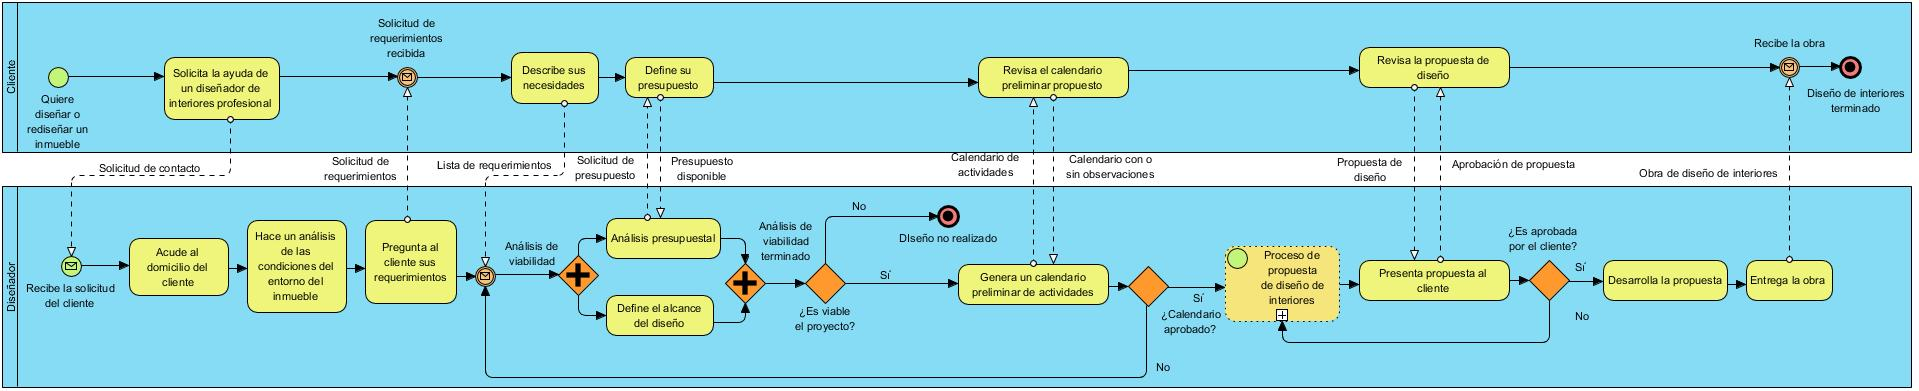
\includegraphics[width=20cm,angle=270,origin=c]{imagenes/marcoteorico/bpmn/proceso_full.jpg}
	\caption{Modelo del proceso de diseño de interiores (Completo).}
	\label{fig:bpmn_antes}
\end{figure}
\newpage

\begin{figure}[!htbp]
	\centering
	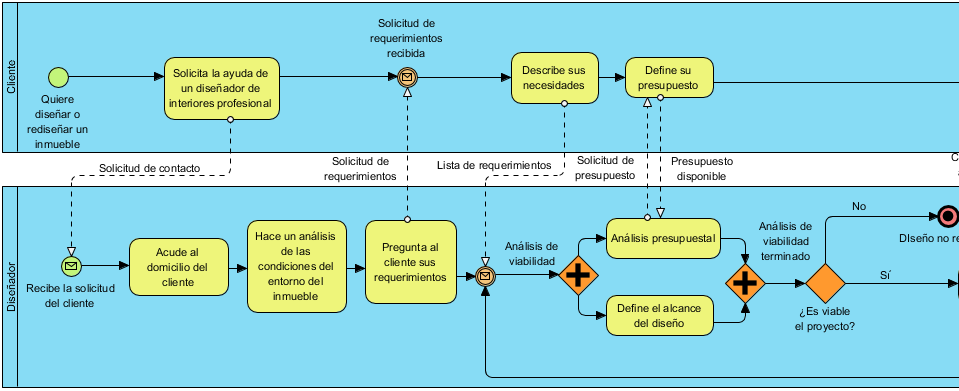
\includegraphics[width=19cm,angle=270,origin=c]{imagenes/marcoteorico/bpmn/proceso_01_01_left.png}
	\caption{Modelo del proceso de diseño de interiores (Segmento I).}
	\label{fig:bpmn_antes}
\end{figure}
\newpage

\begin{figure}[!htbp]
	\centering
	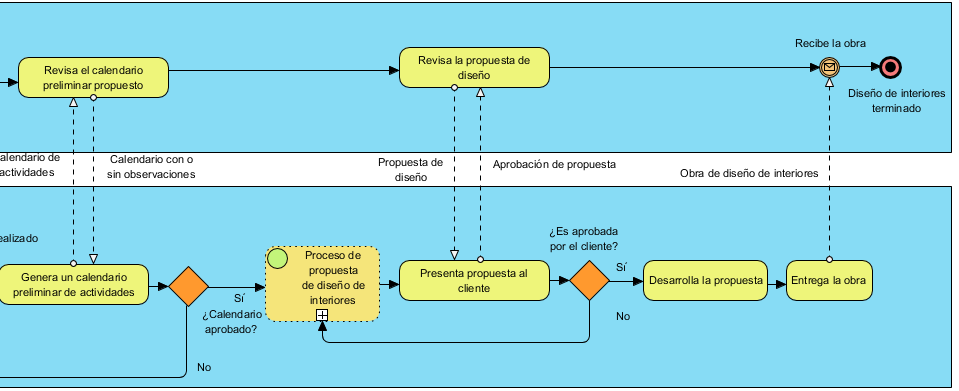
\includegraphics[width=19cm,angle=270,origin=c]{imagenes/marcoteorico/bpmn/proceso_02_01_left.png}
	\caption{Modelo del proceso de diseño de interiores (Segmento II).}
	\label{fig:bpmn_antes}
\end{figure}
\newpage

\begin{figure}[!htbp]
	\centering
	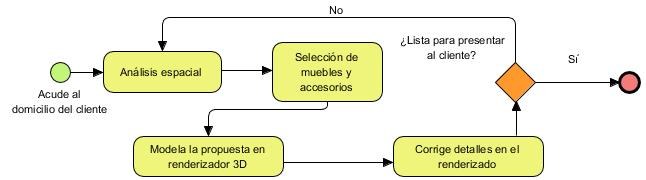
\includegraphics[width=16cm]{imagenes/marcoteorico/bpmn/subproceso.jpg}
	\caption{Subproceso de propuesta de diseño de interiores.}
	\label{fig:subproceso}
\end{figure}
\newpage
	   \section{Problemática}
El diseño de interiores para las personas en general, es un proceso complejo, tardado y tedioso, debido a la implicación del tratamiento superficial y el manejo del volúmen espacial, lo cual puede provocar pérdidas económicas y de tiempo por parte del cliente que compra un mueble y/o por parte de la tienda si se efectúa un proceso de devolución de producto dañando el prestigio de la tienda o sucursal asociada a la venta de estos muebles u objetos.

   
	   \section{Trabajo previo}
Las aplicaciones y proyectos que abordan el problema anteriormente descrito son:

\begin{enumerate}
	\item Canvas (iOS).
	\item Amazon App.
	\item Fingo.
	\item Ikea Place.
	\item TT 2012-B043. Realidad aumentada aplicada a la decoración de interiores.
\end{enumerate}

De forma colectiva, en tales aplicaciones pudimos notar las siguientes características:

\begin{enumerate}
	\item La cámara puede escanear una habitación para conocer los planos donde puede posicionar muebles.
	\item El usuario puede exportar el escaneo tridimensional de una habitación para usarlo en AutoCAD.
	\item Mediante realidad aumentada el usuario puede posicionar un objeto a donde enfoque la cámara del celular.
	\item Existe una posición relativa de los objetos, es decir, si el celular se mueve el objeto permanece en la misma posición.
	\item Se requiere un hardware especial además del dispositivo móvil.
\end{enumerate}

Cabe destacar que Fingo y el TT 2012-B043 utilizan marcadores físicos, colocados en el suelo, sobre los cuales se superponen los objetos tridimensionales, lo cual limita su uso, dado que son dependientes de un elemento externo.\par
Por otro lado, encontramos características que consideramos importantes para resolver el problema planteado, pero ninguna de las aplicaciones anteriores las posee, como son:


\begin{enumerate}
	%\item No están enfocadas a e-Commerce
	\item No existe un gran repertorio de submodelos de objetos
	\item No poseen valores agregados en los objetos en general, por ejemplo, que se muestre el costo de un producto.
	\item No muestra presupuestos generales que indiquen los costos de los productos agregados al entorno de realidad aumentada, ni permite definir un presupuesto inicial que limite los objetos que se van a agregar.
	\item No permiten guardar información relacionada a los entornos de realidad aumentada generados.
\end{enumerate}

En la \textbf{\textit{Tabla 1.1}} podemos apreciar una comparación de las aplicaciones anteriores y la aplicación que planeamos hacer con base en las características previamente descritas:\par

% Please add the following required packages to your document preamble:
% \usepackage{graphicx}
% \usepackage[table,xcdraw]{xcolor}
% If you use beamer only pass "xcolor=table" option, i.e. \documentclass[xcolor=table]{beamer}
\begin{table}[!hbtp]
	\resizebox{\textwidth}{!}{%
		\begin{tabular}{|l|l|l|l|l|l|l|}
			\hline
			\textbf{Características}       & \textbf{Canvas}                                 & \textbf{Tango}           & \textbf{Fingo}           & \textbf{Ikea Place}      & \textbf{TT 2012-B043}    & \textbf{Nuestra App}     \\ \hline
			Escaneo                        & \cellcolor[HTML]{BFBFBF}{\color[HTML]{C0C0C0} } &                          & \cellcolor[HTML]{BFBFBF} & \cellcolor[HTML]{FFFFFF} & \cellcolor[HTML]{BFBFBF} & \cellcolor[HTML]{BFBFBF} \\ \hline
			Exportar                       & \cellcolor[HTML]{BFBFBF}                        &                          &                          & \cellcolor[HTML]{FFFFFF} & \cellcolor[HTML]{FFFFFF} &                          \\ \hline
			Enfoque                        &                                                 & \cellcolor[HTML]{BFBFBF} &                          & \cellcolor[HTML]{BFBFBF} & \cellcolor[HTML]{BFBFBF} & \cellcolor[HTML]{BFBFBF} \\ \hline
			Posición relativa              &                                                 & \cellcolor[HTML]{BFBFBF} &                          & \cellcolor[HTML]{BFBFBF} & \cellcolor[HTML]{FFFFFF} & \cellcolor[HTML]{BFBFBF} \\ \hline
			Hardware externo               & \cellcolor[HTML]{BFBFBF}                        &                          & \cellcolor[HTML]{BFBFBF} & \cellcolor[HTML]{BFBFBF} & \cellcolor[HTML]{BFBFBF} &                          \\ \hline
			Variedad                       &                                                 &                          & \cellcolor[HTML]{BFBFBF} & \cellcolor[HTML]{FFFFFF} & \cellcolor[HTML]{BFBFBF} & \cellcolor[HTML]{BFBFBF} \\ \hline
			Diseños realistas de objetos   &                                                 &                          & \cellcolor[HTML]{BFBFBF} & \cellcolor[HTML]{BFBFBF} & \cellcolor[HTML]{FFFFFF} & \cellcolor[HTML]{BFBFBF} \\ \hline
			Valor agregado                 &                                                 &                          & \cellcolor[HTML]{BFBFBF} & \cellcolor[HTML]{BFBFBF} & \cellcolor[HTML]{FFFFFF} & \cellcolor[HTML]{BFBFBF} \\ \hline
			Presupuesto general            &                                                 &                          &                          &                          &                          & \cellcolor[HTML]{BFBFBF} \\ \hline
			Presupuesto inicial            &                                                 &                          &                          &                          &                          & \cellcolor[HTML]{BFBFBF} \\ \hline
			Guardar información del diseño &                                                 &                          &                          &                          &                          & \cellcolor[HTML]{BFBFBF} \\ \hline
		\end{tabular}%
	}
	\caption{Comparativo de aplicaciones sobre diseño de interiores}
	\label{comparativoestadodelarte}
\end{table}
	   \section{Solución propuesta}
Para mejorar el proceso de diseño de interiores, proponemos desarrollar una aplicación móvil que permita a los usuarios visualizar a través de la realidad aumentada muebles y objetos decorativos en una habitación, eliminando la necesidad de tenerlos físicamente en ella, la cual servirá como herramienta de apoyo en este proceso; así se reducirá el número de etapas del proceso de diseño de interiores volviéndolo más sencillo y rápido.

 
	   \section{Objetivo}
\subsection{Objetivo general}
Desarrollar una aplicación móvil que permita crear entornos virtuales utilizando realidad aumentada en dispositivos móviles para facilitar y agilizar el proceso de diseño de interiores.

\subsection{Objetivos específicos}
\begin{itemize}
	\item Implementar una forma de visualización de muebles utilizando la realidad aumentada.
	\item Desarrollar una nueva propuesta de diseño de interiores para que los diseñadores de interiores puedan presentar a sus clientes.
	\item Poder almacenar las propuestas de diseño de interiores generadas.
	\item Desarrollar una forma para poder presentar análisis presupuestales de diseños de interiores.
	\item Poder agrupar las propuestas de diseño de interiores por cliente y almacenar información del mismo.
	\item Poder ajustar el costo final de los escenarios creados a través de la definición inicial del presupuesto del cliente.
\end{itemize}
	   \section{Justificación}


    \chapter{Marco Teórico }
	El presente trabajo pretende analizar y documentar el desarrollo de una aplicación móvil para el diseño de interiores, por ello las definiciones que a continuación se exponen son necesarias para entender objetivo y el funcionamiento del software.
	
	   \section{Diseño de interiores}
\subsection{Definicion}
El diseño de interiores es una profesión en la cual soluciones creativas y técnicas son aplicadas dentro de una estructura para lograr la construcción de un entorno interno determinado. Éstas soluciones son funcionales, mejoran la calidad de vida de los ocupantes y son aestéticamente atractivas. Los diseños deben apegarse al código y normas requeridos, y fomentar los principios de sustentabilidad ambiental definidos por el edificio o empresa. El objetivo del diseño de interiores es lograr una armonía en los espacios que habitamos y dar confort al usuario de dichos espacios\cite{B01}. \par
El diseño de interiores sigue una metodología sistemática y coordinada que incluye investigación, análisis e integración de conocimientos dentro de un proceso creativo. Dentro ésta metodología podemos ubicar distintos servicios o etapas, dependiendo de la complejidad del trabajo, en las cuales encontramos: definición de los requerimientos funcionales para los espacios de las habitaciones, planeación de espacios interiores, realización de planos de construcción, definición de especificaciones de ubicación, colores y acabados en piso, paredes, materiales, equipo, mobiliario y muebles, administración de contratos de fabricación o instalación, etc.\par
En Estados Unidos el diseño de interiores es la única rama del diseño que está sujeta a las regulaciones federales y la ley gubernamental\cite{B02}.
\subsection{Movimientos en el diseño de interiores}

\subsubsection{Feng shui}
El Feng Shui es un arte utilizado actualmente para alcanzar la armonización de las energías en las casas y los lugares de trabajo, basado en principios milenarios de la sabiduría chin\cite{B26}. Surge de la conjunción de dos ideogramas chinos que significan ``viento" y ``agua", dos conceptos que para las tradiciones de la antigüedad se relacionaban con el flujo y la circulación de la energía vital. Mediante este arte, nos es posible conocer cuál es la perfecta ubicación para edificar una casa, el lugar ideal para colocar cada uno de los muebles, así como también la forma de revertir las energías adversas que puedan afectarnos. El Feng Shui estudia la relación del hombre con la naturaleza y brinda la oportunidad de vivir de acuerdo con los principios que la rigen, y de esta manera, aprovechar esas energías que fluyen por todas partes y pueden influir en nuestro bienestar general.

\subsubsection{Deconstructivismo}
El desconstructivismo es la arquitectura que busca llegar a nuevas formas de expresión al alejarse de las restricciones estructurales y jerarquías funcionales y temáticas, enfocado 
hacia diseños a menudo no rectangulares, fantásticos y aparentemente inconexos\cite{B24}. Tal trabajo a menudo representa una aplicación de las teorías filosóficas  de Jacques Derrida en Francia, que trato de llegar a nuevas ideas en la literatura; esta filosofía se ha aplicado desde finales del siglo 20 a las estructuras arquitectónicas generalmente llamadas arquitecturas deconstructivistas. \par
La arquitectura deconstructivista surge en una exposición, titulada ``Deconstructivist architecture", que Philip Johnson y Mark Wigley organizaron en el museo de Arte Moderno (MoMa) de Nueva York en 1988.

\subsubsection{Diseño Orgánico}
Arquitectura cuyo diseño se establece de acuerdo con los procesos de la naturaleza en lugar de basarse en un diseño ya impuesto. Es una filosofía de diseño propuesta por Frank Lloyd Wright (1867-1959) a comienzos del siglo 20 y en ella afirma que un edificio (y su apariencia) deben de seguir formas que estén en armonía con su entorno natural.\cite{B24}\par  
Los materiales utilizados en el exterior deben ser acoplarse con la ubicación del edificio, relacionando así el edificio con su entorno. Por lo tanto, debe hacerse de baja altura, con techos que sobresalgan para proporcionar protección del sol en el verano y para proporcionar alguna protección contra la intemperie en invierno además se debe de hacer un máxima uso de la luz natural.

\subsection{Fundamentos del diseño de interiores}
El diseño de interiores se ve como una actividad que tiene un punto de inicio (cuando el diseñador y el cliente tienen el primer contacto) y otro al final cuando el proyecto se ha ejecutado.\par
Se debe tomar en cuenta que el diseño de interiores es maleable, es decir, que su realización no está sujeto estrictamente a una serie de reglas. En un caso se puede realizar un determinado proceso, y en otro se puede realizar otro proceso diferente. No existe una solución estandarizada para para todos los casos.\par
Lo más importante es definir el por qué estamos diseñando. Por ejemplo si se está diseñando un armario, se tiene qué saber cuál es el impulso para hacerlo. El diseñador se plantea algunas ideas sobre las funciones que tiene un armario, el uso de la madera reciclada, el del plástico o un nuevo material, y con base a eso, define el objetivo de diseñar el armario.
Otro fundamento importante es la armonía que se busca. Un espacio interior no sólo debe verse bonito, y tener colores agradables a la vista. Cada elemento que compone un espacio debe relacionarse con los demás. Un sillón en una sala de espera debe relacionarse y tener alguna conexión con la mesa de centro. Esta relación puede ser la similitud del acabado de ambos, la ubicación de uno con respecto al otro, etc.
Una habitación debe seguir un esquema de colores bien definido. Dentro de estos esquemas tenemos el monocromático, complementario y análogo, y cada uno deriva del círculo cromático.\par

\textbf{Monocromático}.- Es una selección de colores que funcionen bien juntos. Esto es trabajar con un matiz, y la variación de tintes, tonos, y sombras.
\begin{figure}[h!]
	\centering
	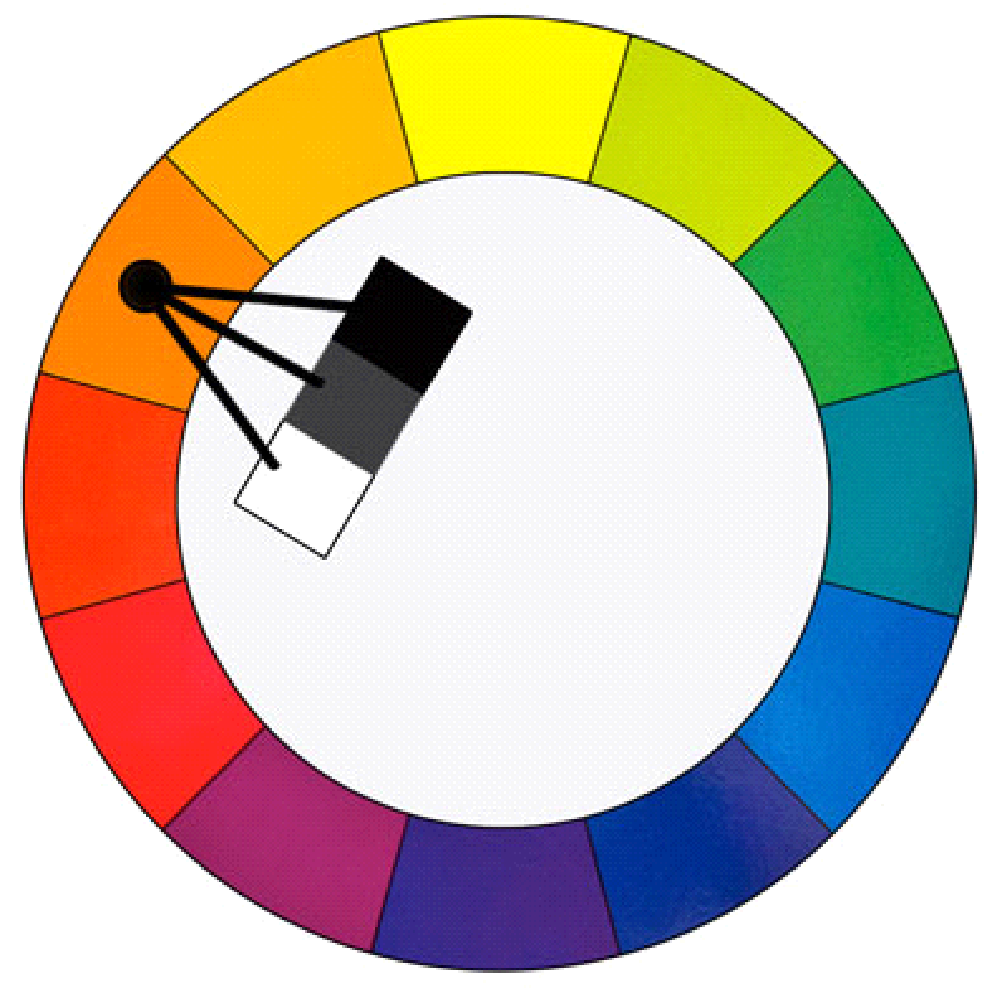
\includegraphics[width=7cm]{imagenes/marcoteorico/disenointeriores/monocromatico.png}
	\caption{Esquema monocromático.\cite{B13}}
	\label{fig:monocromatico}
\end{figure}

\textbf{Complementario}.- Los colores que se encuentran en extremos opuestos del círculo cromático se consideran complementarios. Al combinar estos dos colores, se puede expresar contraste e interés. Son difíciles de usar en grandes cantidades, pero por su contraste son muy buenos para resaltar algo, como un llamado de atención.
\begin{figure}[h!]
	\centering
	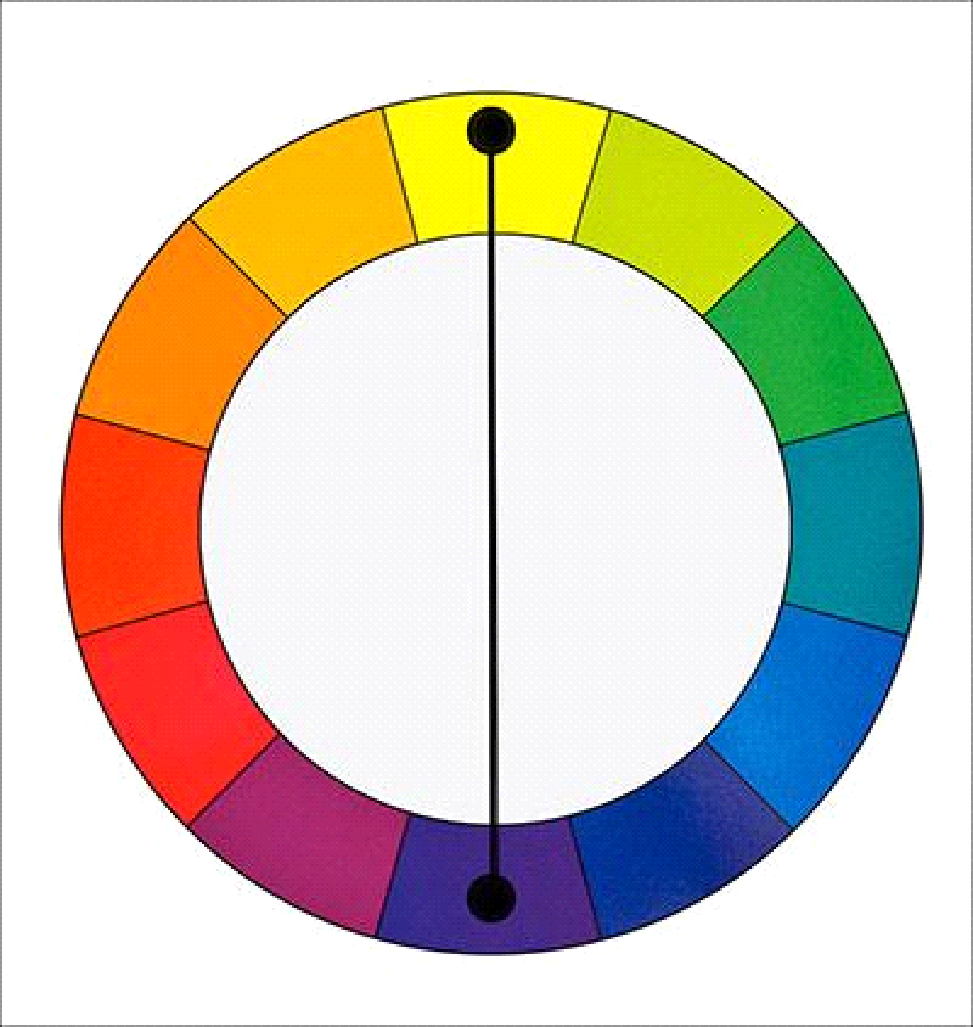
\includegraphics[width=7cm]{imagenes/marcoteorico/disenointeriores/complementario.png}
	\caption{Esquema complementario.\cite{B13}}
	\label{fig:complementario}
\end{figure}

\textbf{Análogo}.- Los colores que se encuentran al lado en el círculo cromático, son agradables juntos. Son la combinación perfecta, ya que son perfectos para cualquier uso, incluso para resaltar y contrastar un elemento específico sin demasiada interrupción. Como regla general, se debe seleccionar un color dominante, un segundo color para sustentar, y un tercer color para acentuar.
\begin{figure}[h!]
	\centering
	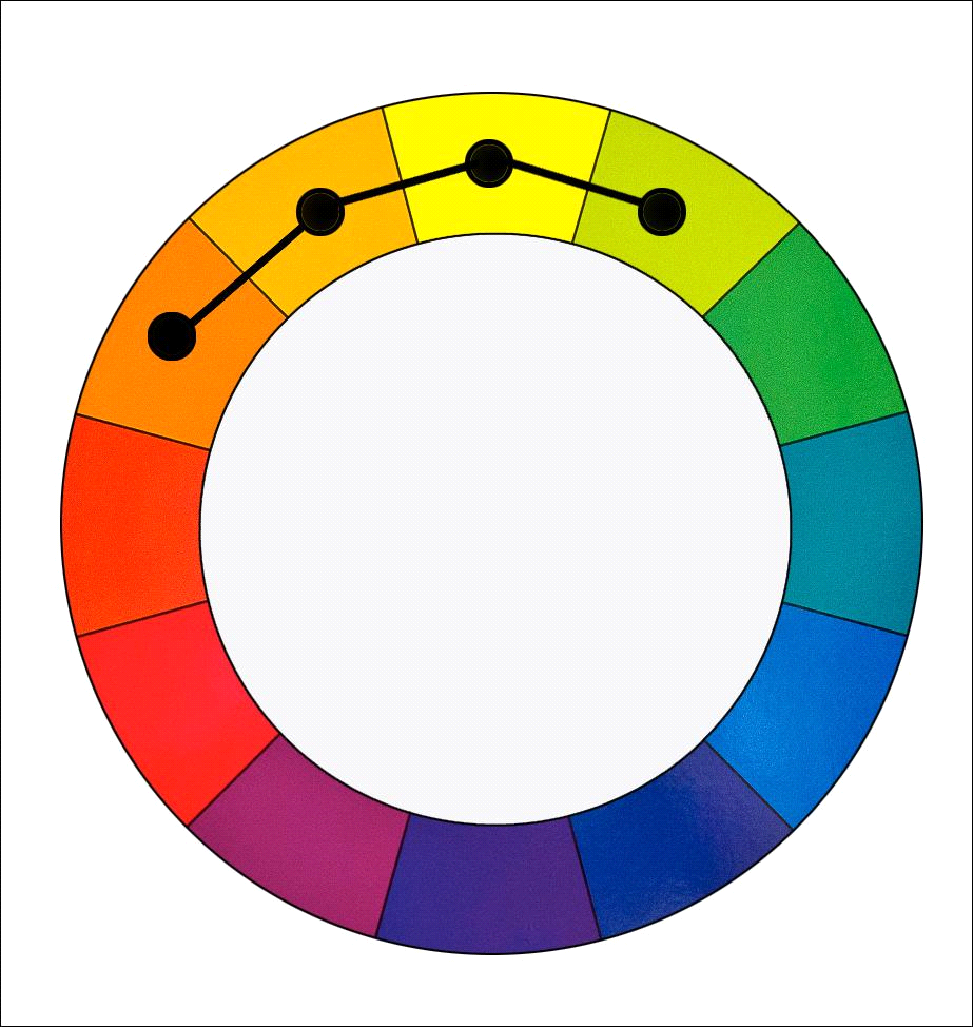
\includegraphics[width=7cm]{imagenes/marcoteorico/disenointeriores/analogo.png}
	\caption{Esquema análogo.\cite{B13}}
	\label{fig:analogo}
\end{figure}


\par 

       \section{Realidad Aumentada}

\subsection{Definición}
\subsection{Tipos de realidad aumentada}
\subsection{Aplicaciones de la realidad aumentada}
\subsection{Impacto de la realidad aumentada}
\subsection{Plataformas de realidad aumentada para dispositivos mófilves}

\subsubsection{Wikitude}
\subsubsection{ARKit}
\subsubsection{Vuforia}
\subsubsection{ARToolKit}
\subsubsection{ARCore}


----------------------------------------------

La mayoría de las veces asociamos los términos de realidad aumentada con la realidad virtual como si fueran lo mismo, sin embargo existen grandes motivos para detallar sus diferencias de software, hardware y de la interacción con los usuarios. \\.\par 

La realidad aumentada (AR) nos permite sobreponer objetos en tercera dimensión sobre una imagen en tiempo real, obteniendo una mezcla de lo real con lo virtual, mejorando la percepción del mundo real de un usuario. Estas imagenes en tiempo real las podemos obtener con las camaras de smartphones, tablets, smart glasses y computadoras. [1] \\. \par

Por otro lado la realidad virtual (VR) se define como un sistema informático que genera en tiempo real representaciones de una realidad es decir, un mundo virtual donde puede llegar a existir una interacción con el usuario. Muchas de estas simulaciones requieren de gafas de VR compatibles con smartphones o gafas especiales como el Gear VR desarrollado por Samsumg en colaboración con Oculus VR. [2][3] \\. \par

A diferencia de la VR, la AR es una tecnología que complementa  la percepción  e interacción  con el mundo real y permite al usuario estar en un entorno aumentado con información generada por computadora. [1] \\. \par

Actualmente, existen dos grandes representantes en estas tecnologías. Tal vez por criterios de marketing diríamos que Google Glass es el representante de la realidad aumentada, mientras que el Oculus Rift de Facebook sería el representante de la realidad virtual. [4]

	   \clearpage
\section{Mobile-D}
\subsection{Definicion \cite{B30}}
Mobile-D es una metodología de desarrollo ágil enfocada al desarrollo de aplicaciones móviles. Está basada en otras tres metodologías:
\begin{itemize}
	\item Extreme Programming.
	\item Crystal.
	\item Rational Unified Process.
\end{itemize}
Mobile-D posee las siguientes características:
\begin{itemize}
	\item \textbf{Fases y ritmo}. Los proyectos son desarrollados en iteraciones que comienzan con un día de planeación.
	\item \textbf{Línea de arquitectura}. La construcción de las aplicaciones se hace con patrones de arquitectura y modelado ágil.
	\item \textbf{Desarrollo de pruebas móviles}. Realiza pruebas automatizadas.
	\item \textbf{Integración continua}. Reduce los tiempos de entrega.
	\item \textbf{Programación en pares}. La programación y las pruebas de la aplicación se realizan en parejas.
	\item \textbf{Métricas}. Durante el desarrollo se pueden obtener datos que puedan medir el rendimiento de los procesos de desarrollo.
	\item \textbf{Proceso de software ágil}. Al final de cada iteración se pueden organizar reuniones con el objetivo de mejorar el proceso de desarrollo.
	\item \textbf{Contacto con cliente}. El cliente participa en las etapas de planeación y liberación de las iteraciones.
	\item \textbf{Enfoque al usuario}. Se hace énfasis en la identificación de las necesidades del usuario final.
\end{itemize}

El desarrollo a través de ésta metodología se realiza a través de iteraciones, y cada una de estas contiene cinco etapas (véase Figura 2.8):
\begin{figure}[h!]
	\centering
	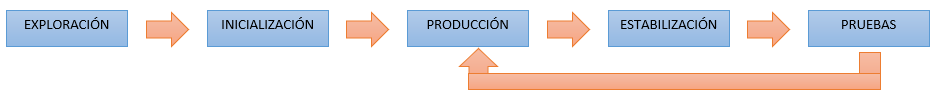
\includegraphics[width=16cm]{imagenes/marcoteorico/mobiled.png}
	\caption{Estructura de Mobile-D. Elaboración propia.}
	\label{fig:mobiled}
\end{figure}
\begin{itemize}
	\item \textbf{Exploración}. El propósito de esta fase es establecer las bases iniciales para el desarrollo del proyecto. Aquí se definen a los involucrados en el proyecto y su participación, el alcance de la aplicación, las iteraciones que se harán en total para todo el proyecto, y pruebas de contexto del software que se planea emplear. Ésta fase se realiza solamente en la primer iteración (iteración 0).
	\item \textbf{Inicialización}. En ésta fase se define el entorno de trabajo del proyecto (las herramientas, versiones y dispositivos que se usarán) y la arquitectura que tendrá el sistema. De igual forma, ésta fase sólo se realiza en la primer iteración (iteración 0).
	\item \textbf{Producción}. En ésta fase se realiza la programación del sistema. Se desarrolla lo planeado en la etapa de exploración.
	\item \textbf{Estabilización}. Si lo desarrollado en la iteración consta de varios módulos, ésta etapa se encarga de unirlos y asegurar la integridad del sistema. Dentro de esta etapa también se realiza la documentación del sistema.
	\item \textbf{Pruebas y correcciones}. Se realizan pruebas a la aplicación verificando que se cumplan los casos de uso, y en caso de haber errores, se corrigen también en esta etapa.
\end{itemize}



    %%%%%%%   ANALISIS   %%%%%%%
	\chapter{Análisis } %CAP\'ITULO 3
En la siguiente sección describe los requerimientos y diagramas de la aplicación. Además, se detallan los diferentes escenarios posíbles.
	
	   \section{Descripción general de la aplicación}
Este sistema móvil sera capaz de  brindarle al usuario final una herramienta que le permita observar muebles virtuales y al mismo tiempo de percibir la realidad obtenida por una cámara,\par
\vspace{5mm}
Se observará un vídeo en tiempo real de la información virtual sobrepuesta dentro del entorno real por medio de la cámara. Las idea es darle una perspectiva más exacta en forma, color, dimensión nuestro mueble u objeto de agrado. Los resultados de obtener esta realidad mezclada es generar acierto, certidumbre y seguridad a las necesidades de un usuario con pretensiones de adquirirlo mediante una compra. Esta aplicación será enfocada al e-Commerce. El comprador potencial seran las mueblerias y establecimientos de venta de articulos de decoracion y el hogar.\par
\vspace{5mm}
\begin{enumerate}[1.]
	\item La aplicación debe ser un sistema móvil capaz de comunicarse con los servicios de AWS (Amazon Web Services). Esta plataforma nos ofrecera todo lo necesario para la persistencia de la información. Este SGDB será el encargado de alojar la información de los usuarios, muebles e imágenes almacenadas cuando sea necesario. 
	\item Los datos registrados por cada usuario dentro de la aplicación será un nombre,correo y contraseña.\par
	\item Cada mueble creado será alojado en formato base64. El tamaño de almacenamiento de cada objeto dependerá de la complejidad, textura, colores, dimensiones y detalles que influyan significativamente en el proceso de renderización en un dispositivo anfitrión.\par
	\item Las imágenes de nuestro mundo real con información virtual de los muebles se podrán almacenar y ademas generar imagenes o capturas de pantalla de la imagen generada por la cámara en el dispositivo.\par
	\item Por otro lado, cada dispositivo anfitrión deberá contar con un mínimo de Hardware y software definido en la sección técnica dentro de este documento, los usuarios que interactúen con la aplicación  deberá contar con los permisos necesarios para  gestionar  la interacción con hardware o software disponible.\par	
\end{enumerate}

	   
\section{Reglas de negocio}
En esta siguiente sección se definen las reglas de negocio que estarán implicadas en el desarrollo del sistema.\par
\subsection{BR1. Unicidad de usuarios}
El email de los usuarios registrados en el sistema deberá ser único e irrepetible, pues constituye parte del par de credenciales de autenticatión al sistema (email y contraseña). Por lo tanto no es posible registrar una nueva cuenta con un email que ya ha sido registrado previamente.

\subsection{BR2. Contraseña segura}
Las contraseñas de las cuentas que se registren deberán cumplir con lo siguiente:
\begin{itemize}
	\item Tener al menos un dígito.
	\item Tener al menos una letra mayúscula.
	\item Tener al menos una letra minúscula.
	\item Tener al menos un caracter especial.
	\item Tener al menos una longitud de 8 caracteres.
\end{itemize}

\subsection{BR3. Seguridad en recuperación de cuenta}
Debe haber un mecanismo que asegure que solamente el usuario de una cuenta pueda reestablecer su contraseña. El mecanismo es el siguiente:
\begin{itemize}
	\item El usuario solicita la recuperación de su cuenta.
	\item Se genera un código de recuperación y se asocia a su cuenta.
	\item El código de recuperación es enviado via email al correo registrado en la cuenta.
	\item Se le solicita al usuario que escriba el código recibido para confirmar su autenticidad.
	\item Se valida que el código ingresado por el usuario es el mismo que el generado previamente.
	\item El usuario podrá volver a definir su contraseña si la validación anterior es correcta.
\end{itemize}

\subsection{BR4. Organización de muebles}
Los muebles estarán organizados dentro de subcategorías, mismas que estarán contenidas en cateogrías, de tal forma que el menú de muebles de la aplicación esté en el siguiente orden jerárquico:
\begin{itemize}
	\item Categoría.
	\item Subcategoría.
	\item Mueble.
\end{itemize}
\subsection{BR5. Impuesto al Valor Agregado en cotizaciones}
Las obras realizadas por diseñadores de interiores profesionales normalmente requieren la emisión de una factura, lo cual implica elevar el precio de la obra un 16\% correspondiente al IVA.
	   	   \section{Actores}

\subsection{Usuario final}
\textbf{Nombre del actor:} \textit{Cliente} \textbf{(Usuario)}\par
\textbf{Definición :} Usuario final y el principal interesado en usar nuestra aplicación. Tendrá los permisos de un usuario estándar, este actor sera el único considerado hasta este momento ya que en iteraciones posteriores se contempla el aumento de usuarios. A continuación se describen las funciones donde interviene la aplicación este usuario.
	   \section{Requerimientos de la aplicación}
La siguiente sección describimos los módulos, detallando la funcionalidad de cada uno y su flujo con sus posibles escenarios.\par

\subsection{Registro de cuenta}
\textbf{Actor :} \textit{Cliente} \par
\textbf{Descripción :} Los usuarios deberán registrase si desean interactuar por completo con todas las funciones disponibles de la aplicación. Este registro se basa en crear una cuenta con tu nombre, correo electrónico y una contraseña.

\subsection{Inicio de sesión}
\textbf{Actor :} \textit{Cliente} \par
\textbf{Descripción :} Los usuarios deberán acceder con sus datos de registro para tener acceso a toda la funcionalidad de la aplicación.

\subsection{Recuperar contraseña}
\textbf{Actor :} \textit{Cliente} \par
\textbf{Descripción :} Los usuarios que olviden su contraseña de acceso deberán solicitarla y posteriormente enviada a su correo electrónico

\subsection{Crear escenario}
\textbf{Actor :} \textit{Cliente} \par
\textbf{Descripción :} Los usuarios podrán crear un escenario, el cual consiste en un conjunto de fotos o videos donde se aprecia el entorno de realidad aumentada generado por el smartphone.

\subsection{Guardar información de escenarios}
\textbf{Actor :} \textit{Cliente} \par
\textbf{Descripción :} Los usuarios podrán guardar información de escenarios como el tipo de habitación que involucra, el tipo de muebles que tiene, el presupuesto del cliente, etc.

\subsection{Guardar información de proyectos}
\textbf{Actor :} \textit{Cliente} \par
\textbf{Descripción :} Los usuarios podrán guardar información de proyectos como los datos del cliente, observaciones de los proyectos, especificaciones del cliente, etc.

\subsection{Definición de presupuesto inicial}
\textbf{Actor :} \textit{Cliente} \par
\textbf{Descripción :} Los usuarios podrán definir un presupuesto al momento de crear un nuevo escenario, el cual irá disminuyendo conforme los muebles sean agregados al escenario. Este presupuesto se mostrará siempre en pantalla.

\subsection{Visualización de cotización}
\textbf{Actor :} \textit{Cliente} \par
\textbf{Descripción :} Al final de la creación de un escenario, los usuarios podrán consultar la cotización del mismo, esto significa, poder saber el precio total del escenario y de qué se compone ese precio. Los usuarios también podrán definir si se aumentará o disminuirá, ya sea por descuentos que se deseen ofrecer, o comisiones que se quieran cobrar.

\subsection{Crear proyecto}
\textbf{Actor :} \textit{Cliente} \par
\textbf{Descripción :} Los usuarios podrán crear proyectos, que no son más que un conjunto de escenarios relacionados.

\subsection{Visualizar escenario}
\textbf{Actor :} \textit{Cliente} \par
\textbf{Descripción :} Los usuarios podrán ver un escenario tomado, donde observaran las imagenes guardas dentro de su smartphone.

\subsection{Tomar foto}
\textbf{Actor :} \textit{Cliente} \par
\textbf{Descripción :} Los usuarios podrán registrar capturas de su experiencia de la realidad aumentada de la aplicación, las cuales conformarán los escenarios.

\subsection{Grabar y almacenar video}
\textbf{Actor :} \textit{Cliente} \par
\textbf{Descripción :} Los usuarios podrán grabar videos de los entornos de realidad aumentada generados, los cuales junto con las fotos, conformarán los escenarios.


\subsection{Consultar muebles}
\textbf{Actor :} \textit{Cliente} \par
\textbf{Descripción :} Los usuarios podrán consultar los muebles disponibles dentro de un catalogo, donde se verá el modelo visualizado en la realidad aumentada.

\subsection{Clasificación de muebles}
\textbf{Actor :} \textit{Cliente} \par
\textbf{Descripción :} Los muebles estarán clasificados por tipo de habitación, tamaño de habitación y color.

\subsection{Colocación de muebles}
\textbf{Actor :} \textit{Cliente} \par
\textbf{Descripción :}  Los usuarios podrán colocar muebles en el entorno de realidad aumentada a partir de un catálogo.

\subsection{Cambio de posición de muebles}
\textbf{Actor :} \textit{Cliente} \par
\textbf{Descripción :}  Una vez colocado un mueble, los usuarios podrán moverlo de lugar seleccionándolo sobre la pantalla y moviéndolo a donde desee.

\subsection{Mostrar distancia entre muebles adyacentes}
\textbf{Actor :} \textit{Cliente} \par
\textbf{Descripción :}  Los usuarios podrán ver las distancias entre muebles para conocer si se encuentran en una posición adecuada, por ejemplo, que no haya alguna obstrucción para caminar.

\subsection{Subir muebles renderizados a la nube}
\textbf{Actor :} \textit{Cliente} \par
\textbf{Descripción :}  Los usuarios podrán subir muebles renderizados a una plataforma en línea de tal forma que puedan ser usados en la aplicación.

\subsection{Cambiar de color a mueble}
\textbf{Actor :} \textit{Cliente} \par
\textbf{Descripción :} Los usuarios podran cambiarle el color a un mueble.

\subsection{Resaltar mueble seleccionado}
\textbf{Actor :} \textit{Cliente} \par
\textbf{Descripción :} Los usuarios seleccionar un mueble tocando la pantalla del celular para realizar modificaciones del mismo. Este objeto se resaltará sobre los demás para que el usuario tenga la certeza de que está modificando el mueble que desea.

\subsection{Mostrar precios de muebles en escena}
\textbf{Actor :} \textit{Cliente} \par
\textbf{Descripción :} Cuando un usuario coloca un mueble, podrá observar su precio en pantalla.

\subsection{Eliminar muebles}
\textbf{Actor :} \textit{Cliente} \par
\textbf{Descripción :} Los usuarios podrán borrar del escenario muebles que previamente han sido colocados. 

   	   \section{Casos de uso}
A continuación se detalla el modelado de las entidades de negocio y su funcionalidad dentro de la aplicación, así mismo su interacción con los actores que intervendrán en la aplicación.\par
\vspace{5mm} 	
\begin{figure}[h!]
	\centering
	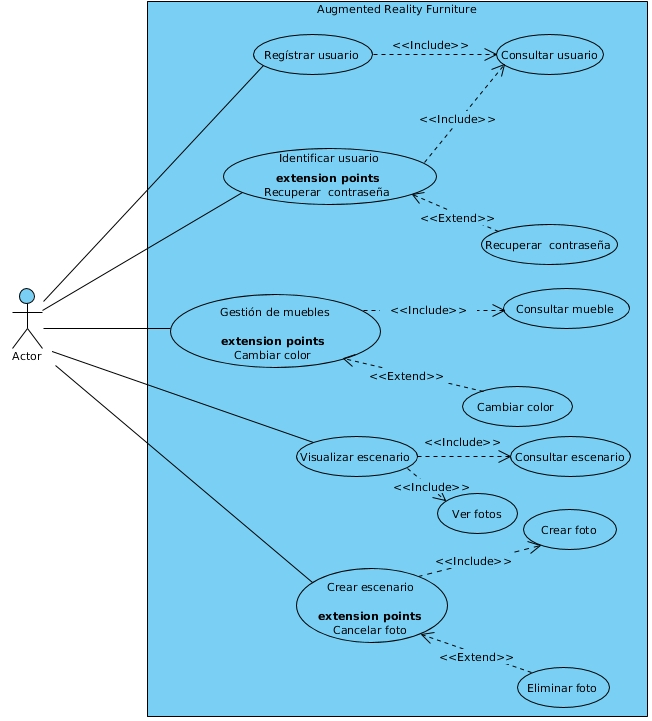
\includegraphics[width=7cm,height=7cm]{imagenes/analisis/casosDeUso.jpg}
	\caption{CU01 Login.\cite{B27}}
	\label{fig:analogo}
\end{figure}  
\newpage

\begin{enumerate}[1.]

\subsection{Login}
\begin{figure}[h!]
	\centering
	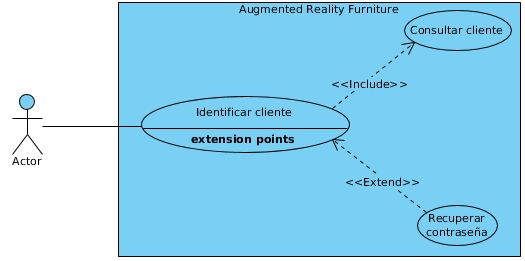
\includegraphics[width=7cm,height=7cm]{imagenes/analisis/login.jpg}
	\caption{CU01 Login.\cite{B27}}
	\label{fig:analogo}
\end{figure}  
\newpage
\item Registrar usuario
\subsection{Registrar usuario} 
\vspace{5mm} 	
\begin{figure}[h!]
	\centering
	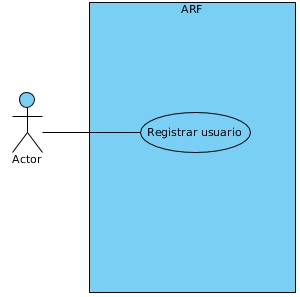
\includegraphics[width=7cm,height=7cm]{imagenes/analisis/registrarUsuario.jpg}
	\caption{CU02 Registrar un usuario.\cite{B27}}
	\label{fig:analogo}
\end{figure} 
\item Recuperar contraseña
\subsection{Recuperar contraseña} 
\vspace{5mm}
\begin{figure}[h!]
	\centering
	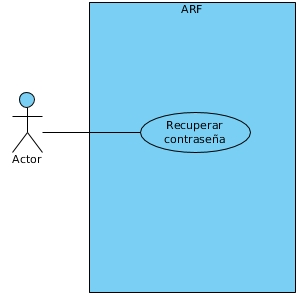
\includegraphics[width=7cm,height=7cm]{imagenes/analisis/recuperarContrasenia.jpg}
	\caption{CU3 Recuperar contrasenia.\cite{B27}}
	\label{fig:analogo}
\end{figure}
\item Gestion de escenario
\subsection{Gestión de escenario} 
\vspace{5mm}
\begin{figure}[h!]
	\centering
	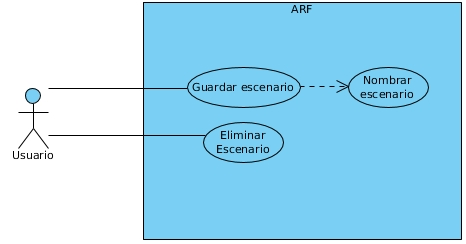
\includegraphics[width=6cm,height=6cm]{imagenes/analisis/Escenario.jpg}
	\caption{CU04 Gestionar escenarios\cite{B27}}
	\label{fig:analogo}
\end{figure}

\item Visualizacion de escenario
\subsection{Visualización de escenario} 
\vspace{5mm} 
\begin{figure}[h!]
	\centering
	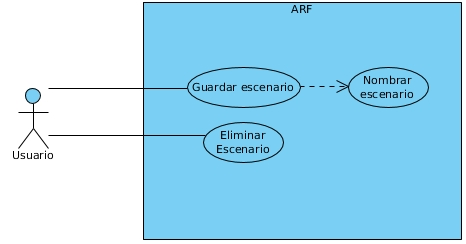
\includegraphics[width=7cm,height=7cm]{imagenes/analisis/Escenario.jpg}
	\caption{Visualizacion de escenario \cite{B27}}
	\label{fig:analogo}
\end{figure}
\end{enumerate}
   	   \newpage
\section{Diagramas de secuencia}
A continuación se describe la interacción de nuestras entidades de negocio y el ciclo de vida que tendrán en la aplicación. También se detalla la interacción,mensajes y la lógica implementada por cada uno de los diferentes escenarios.\par
\subsection{Registro}
El registro de un usuario nuevo consiste en capturar el correo, nombre y una contraseña. Esta captura sera tratada como un JSON el cual viajara atravéz de un método POST. Gateway se encargara de redirigir esta petición al servicio de registro. Este servicio viajara hacia RDS donde se enviara un INSERT para registrar los datos. 
\vspace{5mm}
\begin{figure}[h!]
	\centering
	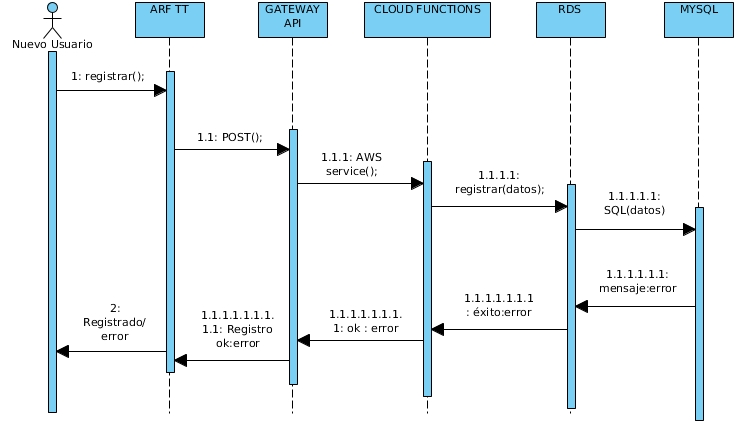
\includegraphics[width=14cm,height=8cm]{imagenes/analisis/DSregistrarUsuario.jpg}
	\caption{Diagrama de secuencia - Registrar usuario.}
	\label{fig:analogo}
\end{figure} 
\vspace{5mm}\par
Si el usuario y la contraseña se encuentra repetido, se enviara un mensaje de error, como se muestra en la figura 3.7
\newpage
\subsection{Login}
La validación de credenciales comienza con capturar el correo y contraseña  de un usuario registrado. Esta información sera tratada como un objeto JSON, el cual se mandara por una método POST. La API Gateway direccionara la petición a un Servicio AWS y  comparara la información en la instancia creada en RDS de un motor de base de datos MySQL. RDS se encargara de generar la conexión y consulta a la base de datos.
\vspace{5mm}
\begin{figure}[h!]
	\centering
	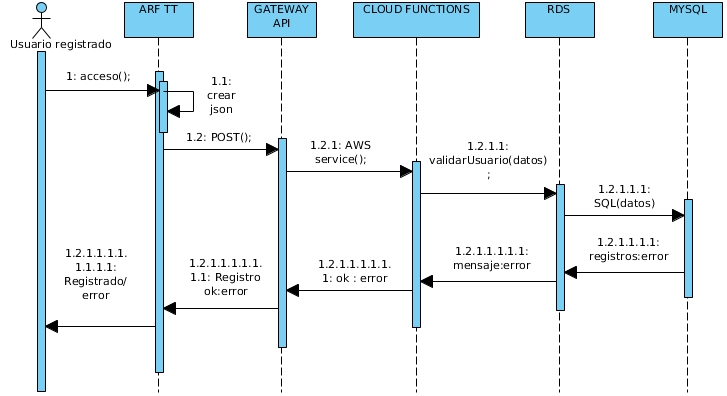
\includegraphics[width=14cm,height=8cm]{imagenes/analisis/DSacceso.jpg}
	\caption{Diagrama de secuencia - Registrar Acceso.}
	\label{fig:analogo}
\end{figure} 
\vspace{5mm} \par
La petición regresara con un mensaje si hubo coincidencia, de lo contrario se enviara un error a la interfaz de usuario.
\newpage
\subsection{Recuperar contraseña}\par
La recuperación de credenciales inicia con la función recuperar, en ella se captura el correo de un usuario y posteriormente lo procesa a un objeto JSON. Esta información se mandara en un método POST. La API Gateway envía la petición a un Servicio AWS y en la instancia creada en RDS procesa un script que comparara el correo con la  información de MySQL, buscando alguna coincidencia. Si existe una coincidencia exacta, MySQL enviará el registro en un mensaje con la contraseña.
\vspace{5mm}
\begin{figure}[h!]
	\centering
	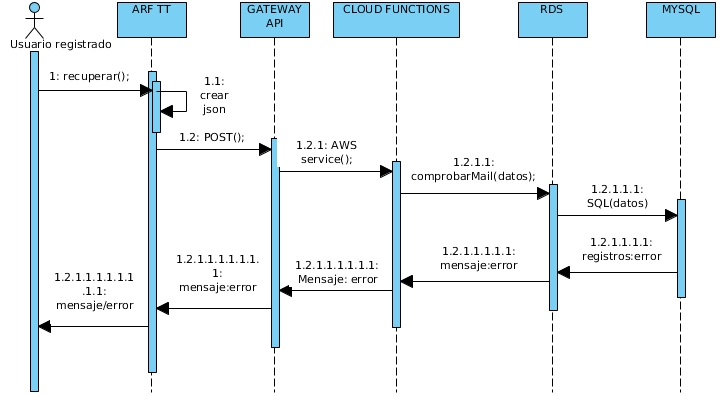
\includegraphics[width=14cm,height=8cm]{imagenes/analisis/DSrecuperarContra.jpg}
	\caption{Diagrama de secuencia - Recuperar contraseña.}
	\label{fig:analogo}
\end{figure}
\vspace{5mm} \par
Si no existe coincidencia se manda un mensaje de error. RDS se encargara de generar la conexión y consulta con el servicio de Amazon Web Services y nuestra instancia de MySQL en RDS.
\newpage
\subsection{Gestión de muebles}
La visualización y edición del color de un mueble inicia desde un menú con los muebles disponibles, cuando un actor selecciona un mueble este dispara una acción donde opcionalmente podrá editar el color. El actor después de seleccionar un color valido enviara la información a los servicios AWS donde se tienen almacenados los muebles, esta información será enviada de regreso para visualizar este objeto con la realidad aumentada de la aplicación.
\vspace{5mm}
\begin{figure}[h!]
	\centering
	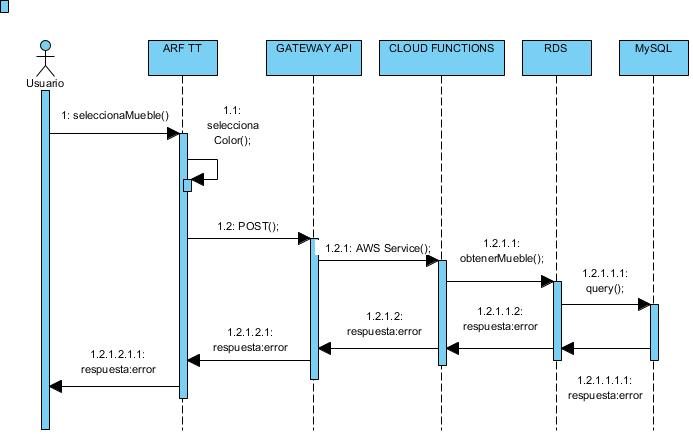
\includegraphics[width=14cm,height=8cm]{imagenes/analisis/DSgestionMuebles.jpg}
	\caption{Diagrama de secuencia -Gestión de muebles.}
	\label{fig:analogo}
\end{figure}
\vspace{5mm} \par
Si ocurre un error desde el servidor se envía un código de error donde se notificara al usuario que no se encuentra disponible.
\newpage
\subsection{Guardar escenario}
La creación y guardado de un escenario inicia cuando se comienza a capturar la realidad aumentada de un mueble, la acción que dispara este proceso será la de guardar escenario, la función tiene como parámetros el identificador del usuario, el nombre del escenario y una colección de imágenes en formato Base64. Esta función procesa las imágenes a binario para su posterior persistencia en S3 Bucket (Simple Storage Service).
\vspace{5mm}
\begin{figure}[h!]
	\centering
	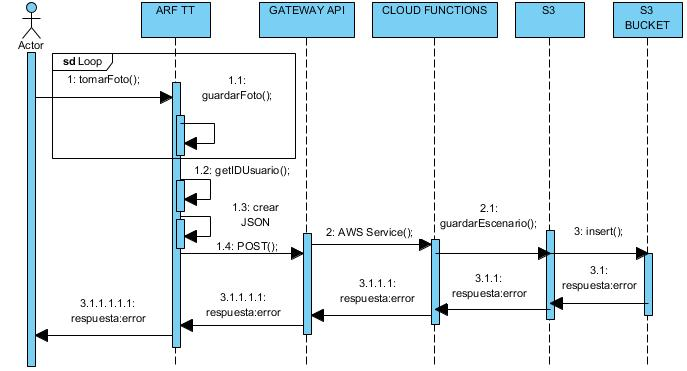
\includegraphics[width=14cm,height=8cm]{imagenes/analisis/DSguardarEscenario.jpg}
	\caption{Diagrama de secuencia - Guardar escenario.}
	\label{fig:analogo}
\end{figure}
\vspace{5mm}\par
El S3 envia un mensaje de éxito o error de la persistencia, el usuario observara la notificación de guardado satisfactorio. En dado caso que la petición sea incorrecta se enviara una notificación de guardado fallído.
\newpage
\subsection{Visualizar escenario}
La visualización de un escenario se dispara cuando el actor selecciona la opción visualizar escenario. La petición se envía por los servicios de AWS que consulta el bucket S3, este a su vez hace la consulta de la información con MySQL, si encuentra una coincidencia se obtiene los nombres y las URL de las imágenes guardadas. Esta información viaja de regreso para que sea visualizada en la pantalla de la aplicación.
\vspace{5mm}
\begin{figure}[h!]
	\centering
	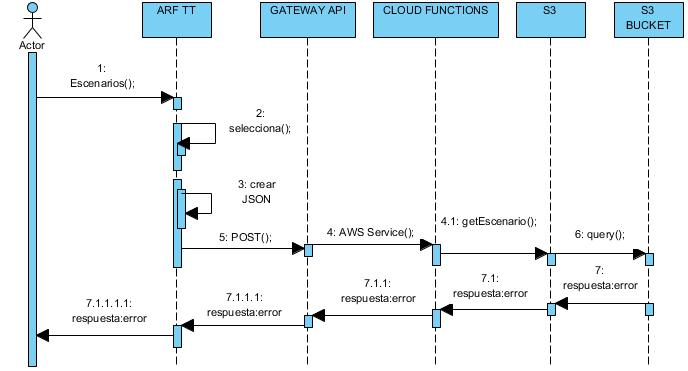
\includegraphics[width=14cm,height=8cm]{imagenes/analisis/DSvisualizarEscenario.jpg}
	\caption{Diagrama de secuencia - Visualizar escenario.}
	\label{fig:analogo}
\end{figure} 
\vspace{5mm} \par 
Si la petición no encuentra alguna coincidencia dentro de S3 se envía un código de error, informando que no existen escenarios para visualizar.





	%%%%%%%   DESARROLLO   %%%%%%%
	\chapter{Desarrollo}

En este capítulo se describirá el proceso de desarrollo del trabajo terminal de acuerdo a la metodología Mobile-D, de tal forma que estará divido en capítulos según las iteraciones que se vayan realizando.\par
		\section{Iteración 0}
\subsection{Exploración}
En este apartado se definirá el alcance del proyecto, los recursos u herramientas a usar, y las personas involucradas en su desarrollo, así como las pruebas de contexto realizadas en las tecnologías que usaremos.


\subsubsection{Pruebas de contexto}
Con el fin de conocer las capacidades de las plataforma ARCore y Vuforia (excluyendo ARKit debido a que su desarrollo es enfocado a sistemas iOS, ARToolkit porque no se centra en dispositivos móviles y a Wikitude por su reducido número de dispositivos compatibles), se realizaron pruebas de contexto definiendo las siguientes especificaciones:
\begin{itemize}
	\item Nombre del dispositivo en el que se realizó
	\item Fecha de prueba
	\item Versión de la tecnologia SDK
	\item Versión de Android
\end{itemize}
Por otro lado cada prueba se realizó tomando en cuenta las siguientes características:
\begin{itemize}
	\item \textbf{Posición Cardinal}.- Define si un objeto virtual puede visualizarse desde los cuatro puntos cardinales (norte, sur, este, oeste) y desde la parte superior del mismo, cuando la cámara gira alrededor del objeto mientras lo enfoca.
	\item \textbf{Tamaño relativo}.- Define si un objeto cambia su tamaño en el entorno virtual dependiendo de la distancia a la que se acerque o se aleje la cámara. Cuando la cámara se acerca, el objeto deberá aumentar su tamaño, y viceversa, como si se tratase de un objeto real.
	\item \textbf{Luminosidad}.- Define el grado de oscuridad de un objeto a determinada luz, es decir, cuando la luz en el ambiente real es alta, el objeto se verá iluminado, en caso contrario cuando haya escasa luz, el objeto se oscurecerá.
	\item \textbf{Superficie}.- Describe en qué superficies el objeto virtual es puesto, si fue posible su superposición en este material y qué comportamiento tiene en cada una de estas.
	\item \textbf{Memoria de objetos}.- Define si los objetos virtuales se conservan en la memoria cuando la cámara pierde su enfoque en ellos y los vuelve a enfocar. También describe si los objetos conservaron su posición tras el re-enfoque.
	\item \textbf{Capacidad máxima de objetos}.- Define el número de objetos virtuales que pueden ser mostrados en escena sin que el rendimiento de la aplicación caiga considerablemente.
	\item \textbf{Distancia}.- Define la distancia a la que se encuentra la cámara de un objeto virtual sin que éste desaparezca o sin que su resolución baje considerablemente.
\end{itemize}
\noindent

\subsubsection{ARcore}
\begin{table}[H]
	\centering
	\begin{tabular}{|c|c|}
		\hline
		\multicolumn{2}{|c|}{Especificaciones de prueba}   \\ \hline
		\textbf{DISPOSITIVO}              & Moto G6 XT1925 \\ \hline
		\textbf{FECHA}                    & 2018/08/25     \\ \hline
		\textbf{VERSIÓN DE SCENEFORM SDK} & V1.4.0         \\ \hline
		\textbf{VERSIÓN DE ARCORE SDK}    & V1.4.0         \\ \hline
		\textbf{VERSIÓN DE ANDROID}       & V8.0.0 (Oreo)  \\ \hline
	\end{tabular}
	\captionsetup{justification=centering}
	\caption{Especificaciones de prueba Arcore en Moto G6}
\end{table}

\textbf{Posición cardinal} \par
El objeto virtual se pudo apreciar con claridad desde los cuatro puntos cardinales y la vista superior. El ángulo de visualización del objeto al mover la cámara cambiaba a la perfección, dando una buena percepción de realismo.

%%IMAGENES DE PUNTOS CARDINALES
\begin{figure}[!htbp]
	\begin{minipage}{0.48\textwidth}
	\centering
		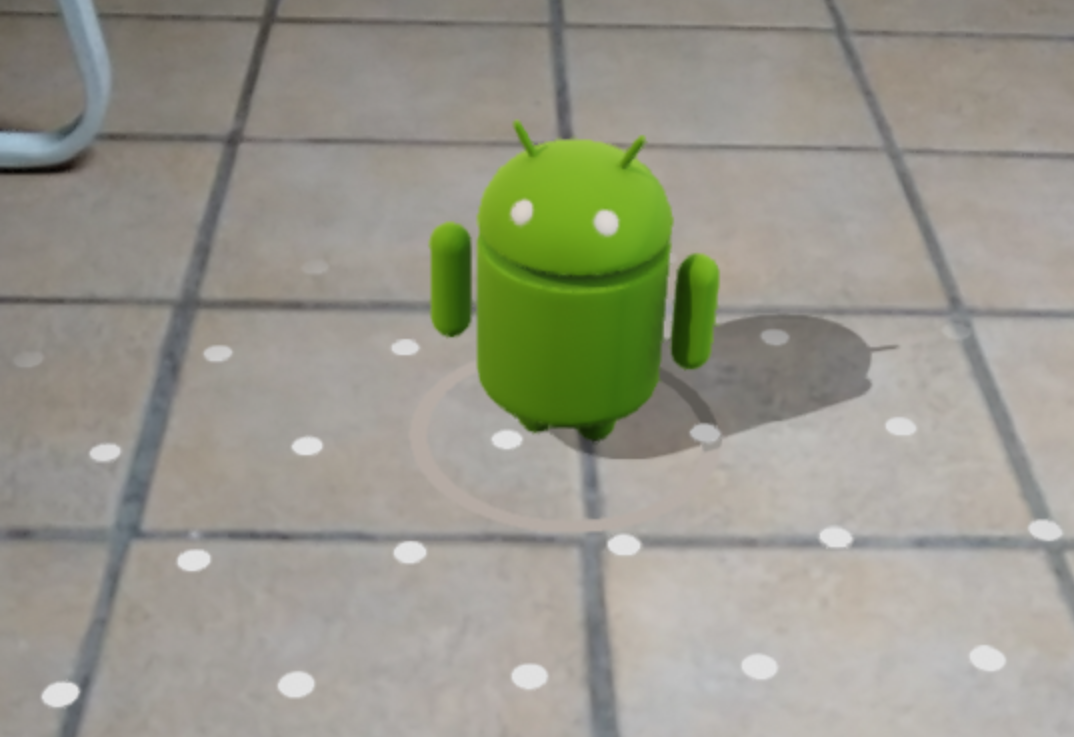
\includegraphics[width=8cm]{desarrollo/secciones/pruebas/motog6/img/NORTE.png}
		\caption{Posición Norte}
		\label{fig:motog6norte}
	\end{minipage}\hfill
	\begin{minipage}{0.48\textwidth}
	\centering
	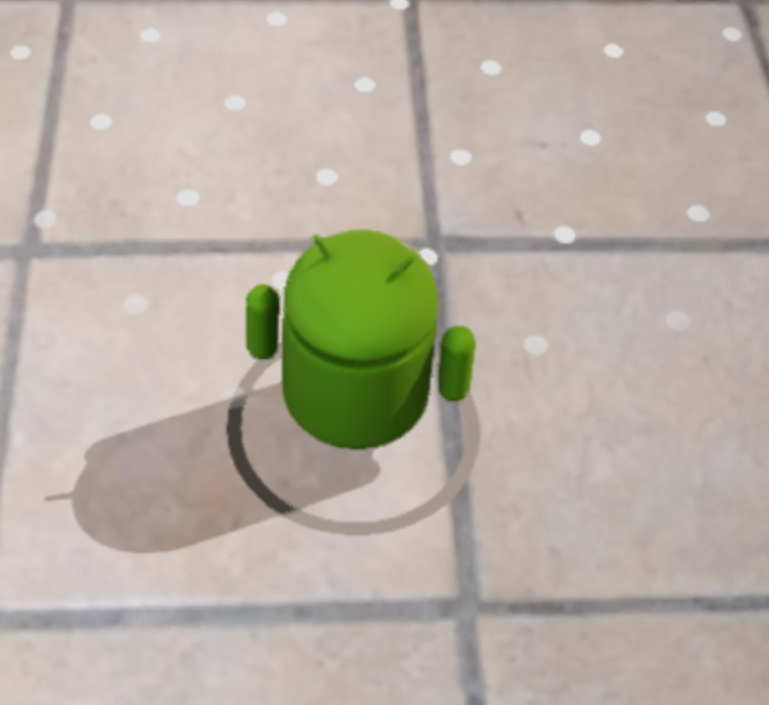
\includegraphics[width=8cm]{desarrollo/secciones/pruebas/motog6/img/SUR.png}
	\caption{Posición Sur}
	\label{fig:motog6sur}
	\end{minipage}\hfill
\end{figure}

\begin{figure}[!htbp]
	\begin{minipage}{0.48\textwidth}
		\centering
		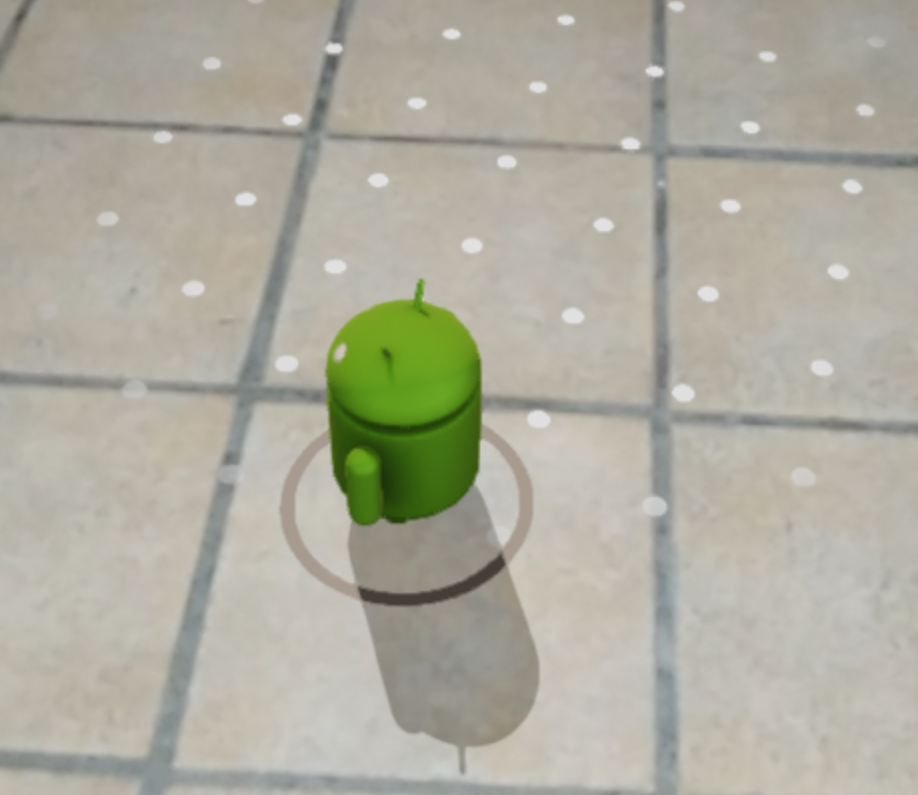
\includegraphics[width=8cm]{desarrollo/secciones/pruebas/motog6/img/ESTE.png}
		\caption{Posición Este}
		\label{fig:motog6norte}
	\end{minipage}\hfill
	\begin{minipage}{0.48\textwidth}
		\centering
		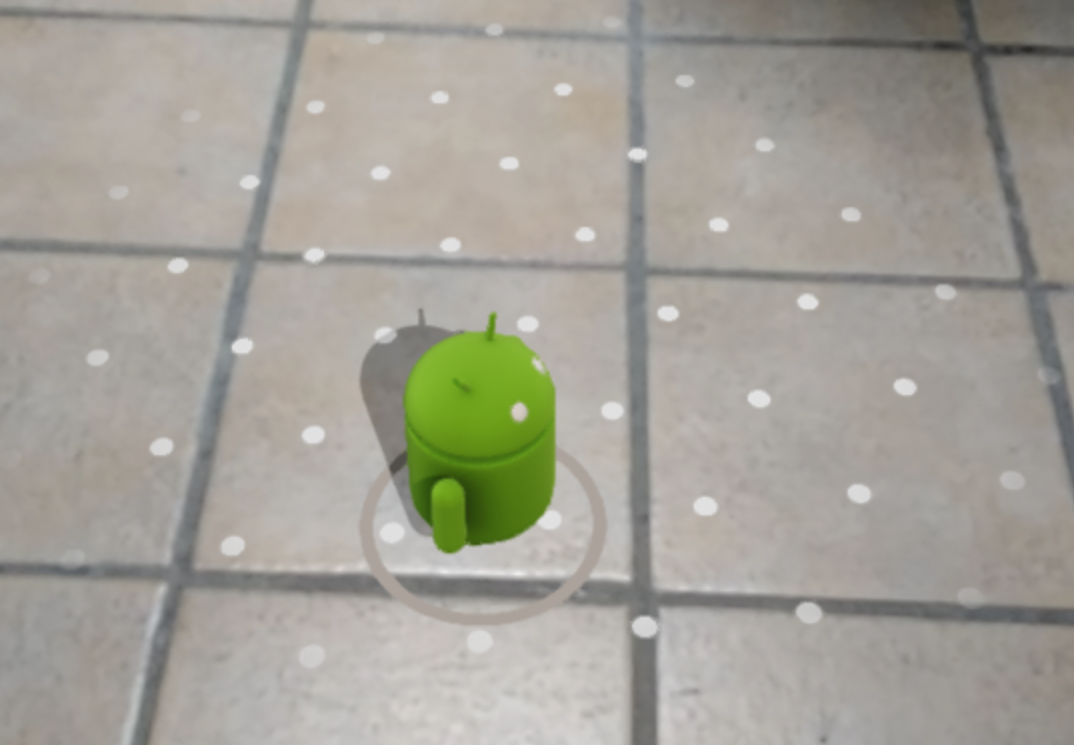
\includegraphics[width=8cm]{desarrollo/secciones/pruebas/motog6/img/OESTE.png}
		\caption{Posición Oeste}
		\label{fig:motog6oeste}
	\end{minipage}\hfill
\end{figure}

\textbf{Tamaño relativo} \par
Al acercar o alejar la cámara el objeto virtual variaba su tamaño de forma adecuada, como si el objeto realmente estuviera en la posición donde fue superpuesto.


\begin{figure}[!htbp]
	\begin{minipage}{0.48\textwidth}
		\centering
		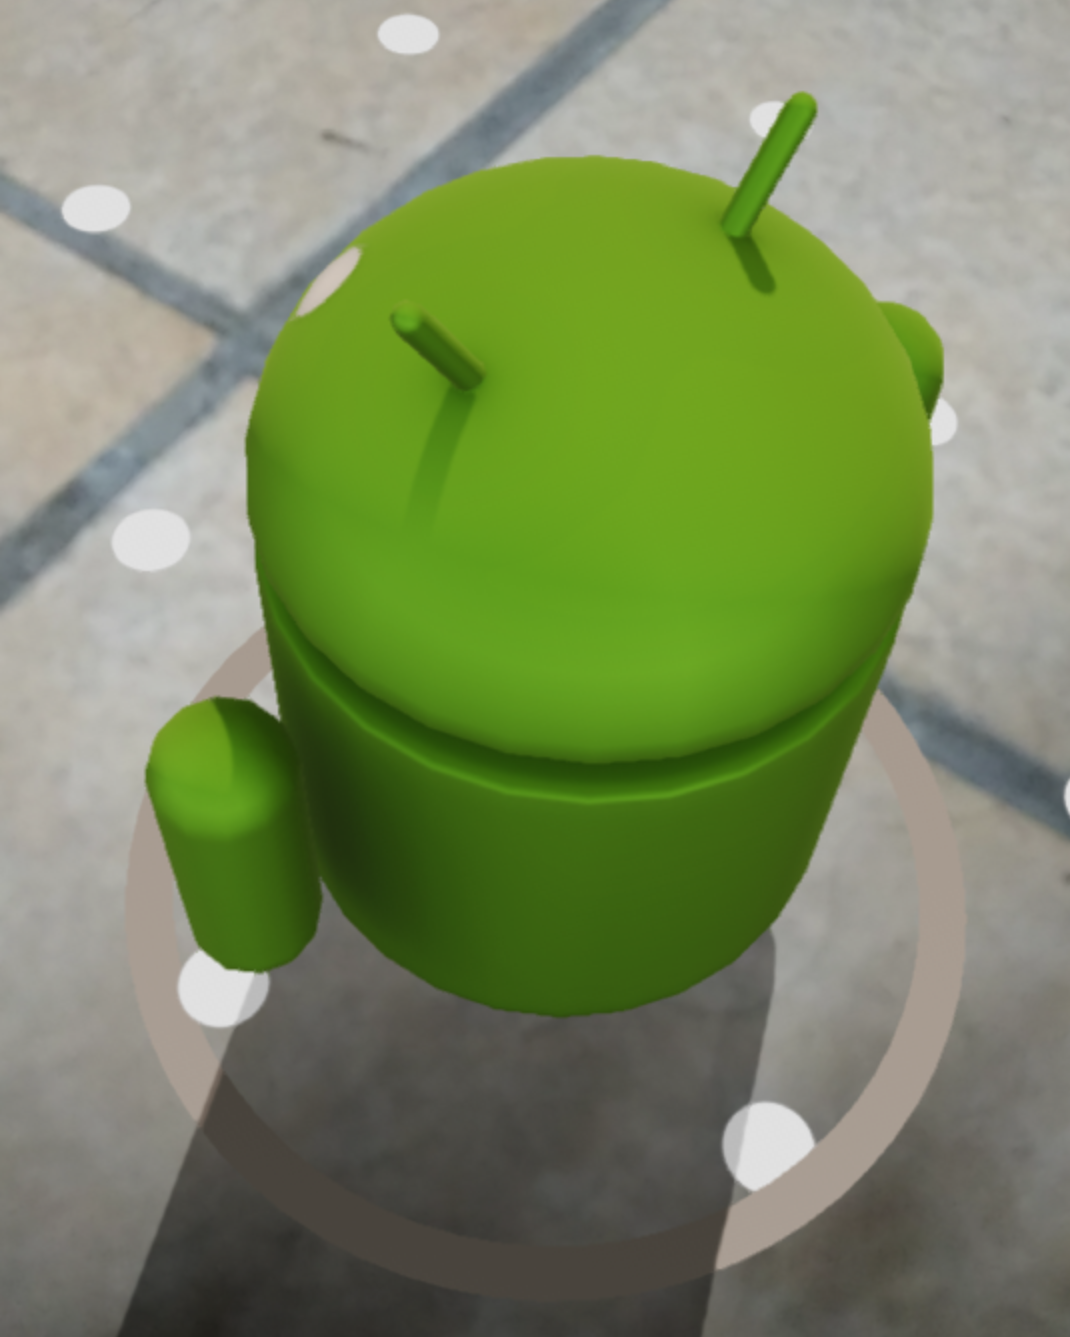
\includegraphics[width=8cm]{desarrollo/secciones/pruebas/motog6/img/CERCA.png}
		\caption{Objeto visto de cerca}
		\label{fig:motog6cerca}
	\end{minipage}\hfill
	\begin{minipage}{0.48\textwidth}
		\centering
		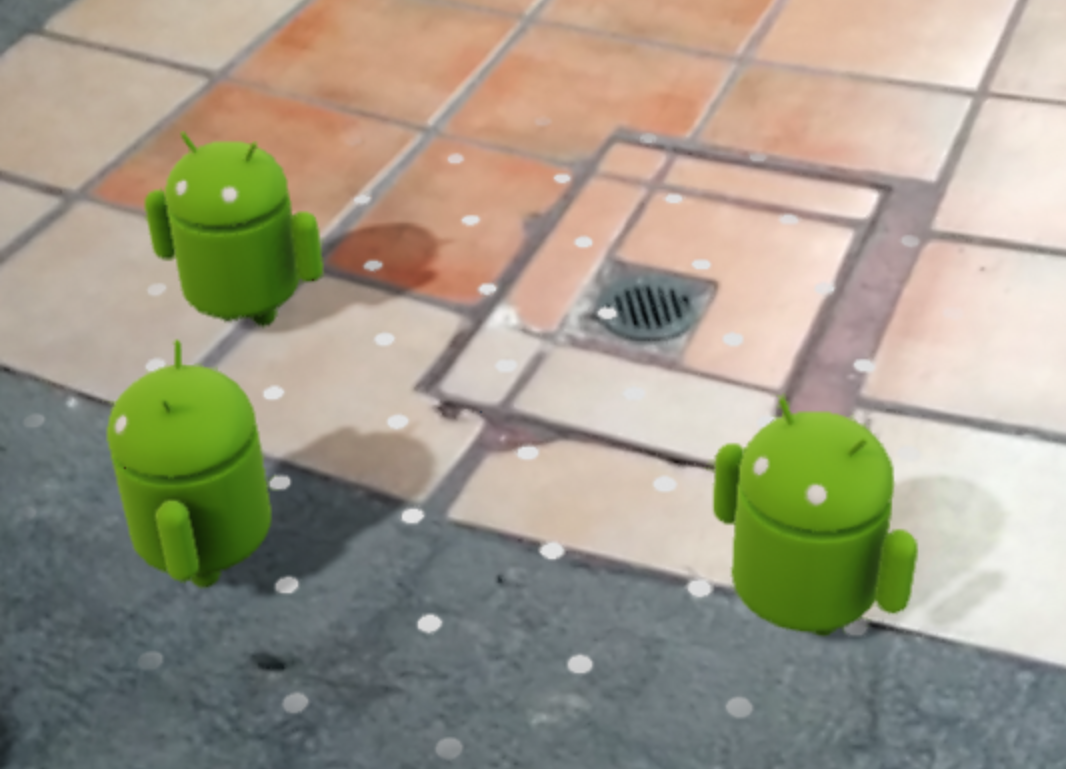
\includegraphics[width=8cm]{desarrollo/secciones/pruebas/motog6/img/LUZALTA.png}
		\caption{Luz alta}
		\label{fig:motog6lalta}
	\end{minipage}\hfill
\end{figure}

\textbf{Luminosidad} \par
Al poner el objeto virtual en entornos con diferente cantidad de luz, la cantidad de luz en el objeto virtual también variaba. En un entorno con ausencia casi total de luz el objeto apenas era perceptible, mientras que en un entorno con bastante luz, el objeto se veía altamente iluminado.

\begin{figure}[!htbp]
	\begin{minipage}{0.48\textwidth}
		\centering
		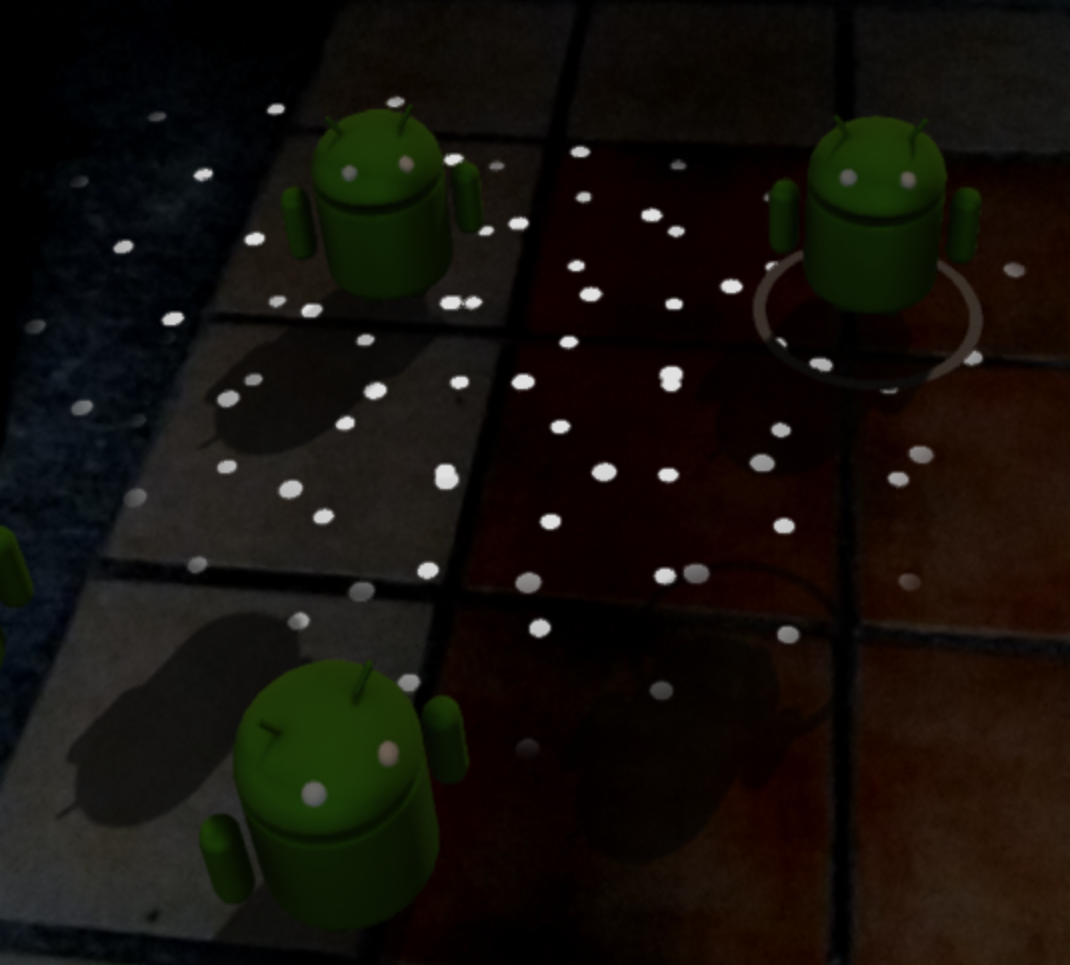
\includegraphics[width=8cm]{desarrollo/secciones/pruebas/motog6/img/LUZBAJA.png}
		\caption{Luz baja}
		\label{fig:motog6lbaja}
	\end{minipage}\hfill
	\begin{minipage}{0.48\textwidth}
		\centering
		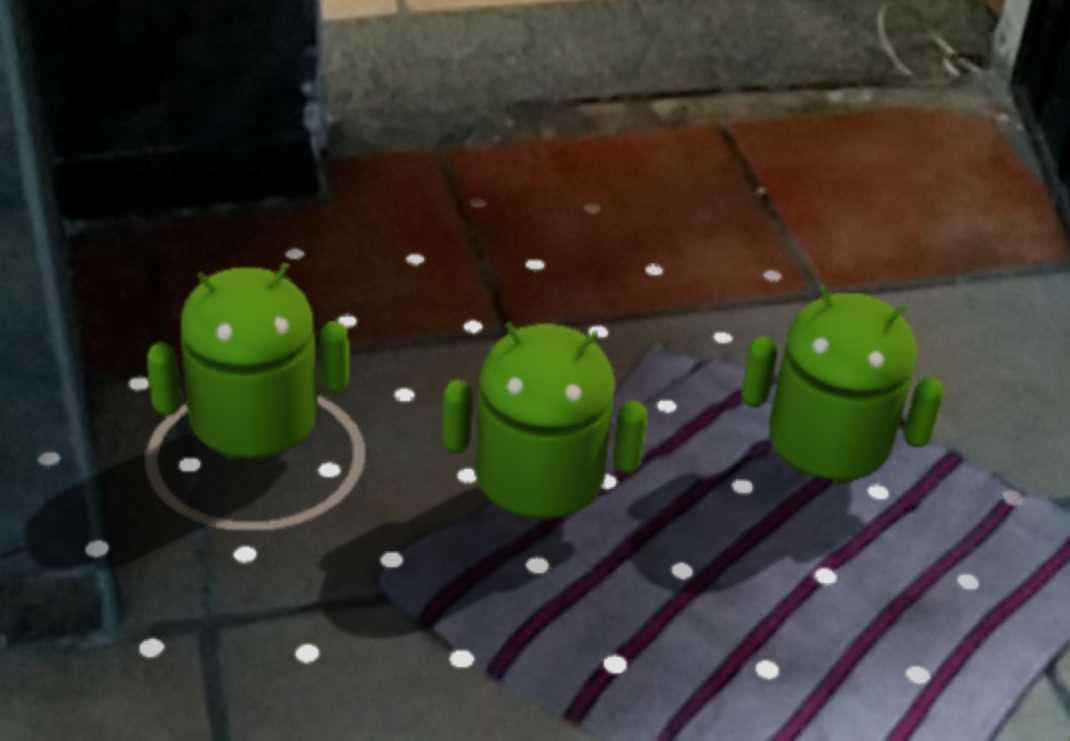
\includegraphics[width=8cm]{desarrollo/secciones/pruebas/motog6/img/LUZMEDIA.png}
		\caption{Luz media}
		\label{fig:motog6lmedia}
	\end{minipage}\hfill
\end{figure}

\textbf{Superficie} \par
Se probó posicionar el objeto virtual en cuatro superficies: concreto gris, concreto blanco, azulejo y vidrio.\par
Concreto gris.- El objeto se pudo posicionar a la perfección.\par
Concreto blanca.- El objeto no se pudo posicionar. La maya de puntos ni si quiera era detectada en ésta superficie debido a la ausencia de texturas.\par
Azulejo.- El objeto se pudo posicionar a la perfección.\par
Vidrio.- El objeto no pudo ser posicionado en ésta superficie debido a las propiedades reflejantes que posee.\par

\begin{figure}[!htbp]
	\begin{minipage}{0.48\textwidth}
		\centering
		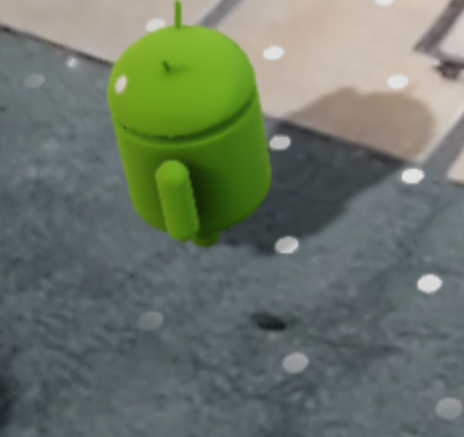
\includegraphics[width=8cm]{desarrollo/secciones/pruebas/motog6/img/CONCRETO.png}
		\caption{Objeto colocado en concreto}
		\label{fig:motog6concreto}
	\end{minipage}\hfill
	\begin{minipage}{0.48\textwidth}
		\centering
		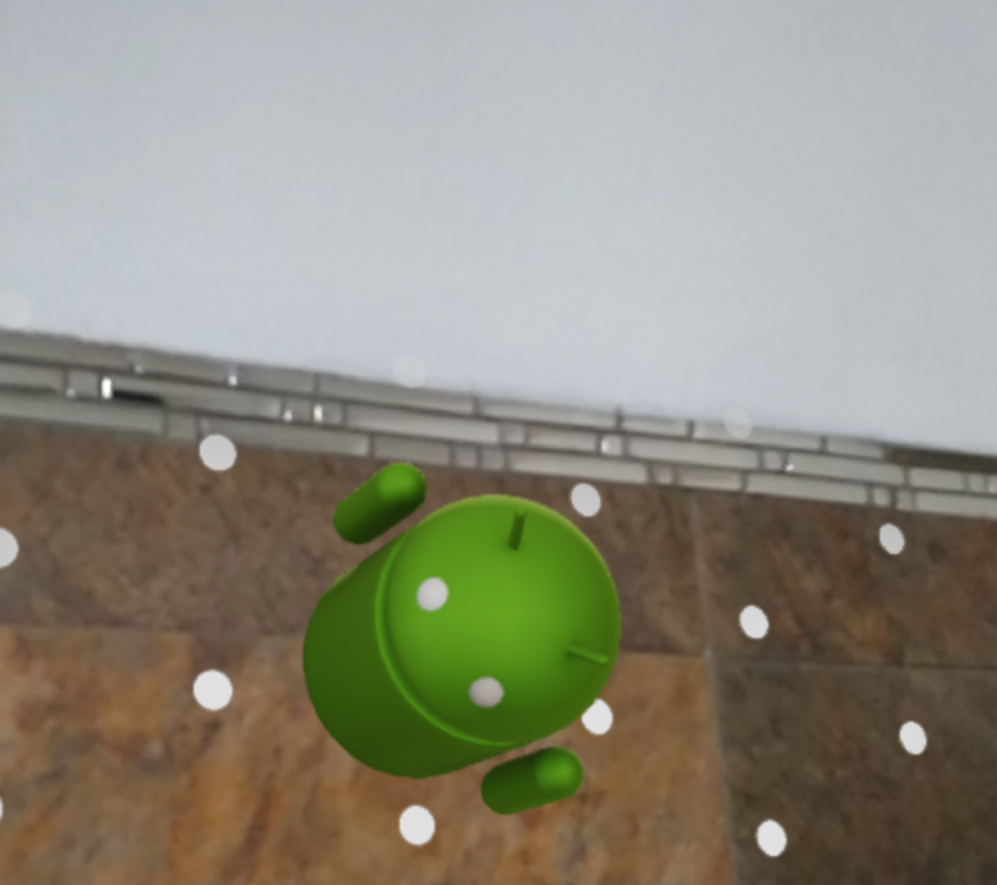
\includegraphics[width=8cm]{desarrollo/secciones/pruebas/motog6/img/SUPBLANCA.png}
		\caption{Objeto colocado en superficie blanca}
		\label{fig:motog6supblanca}
	\end{minipage}\hfill
\end{figure}

\begin{figure}[H]
	\begin{minipage}{0.48\textwidth}
		\centering
		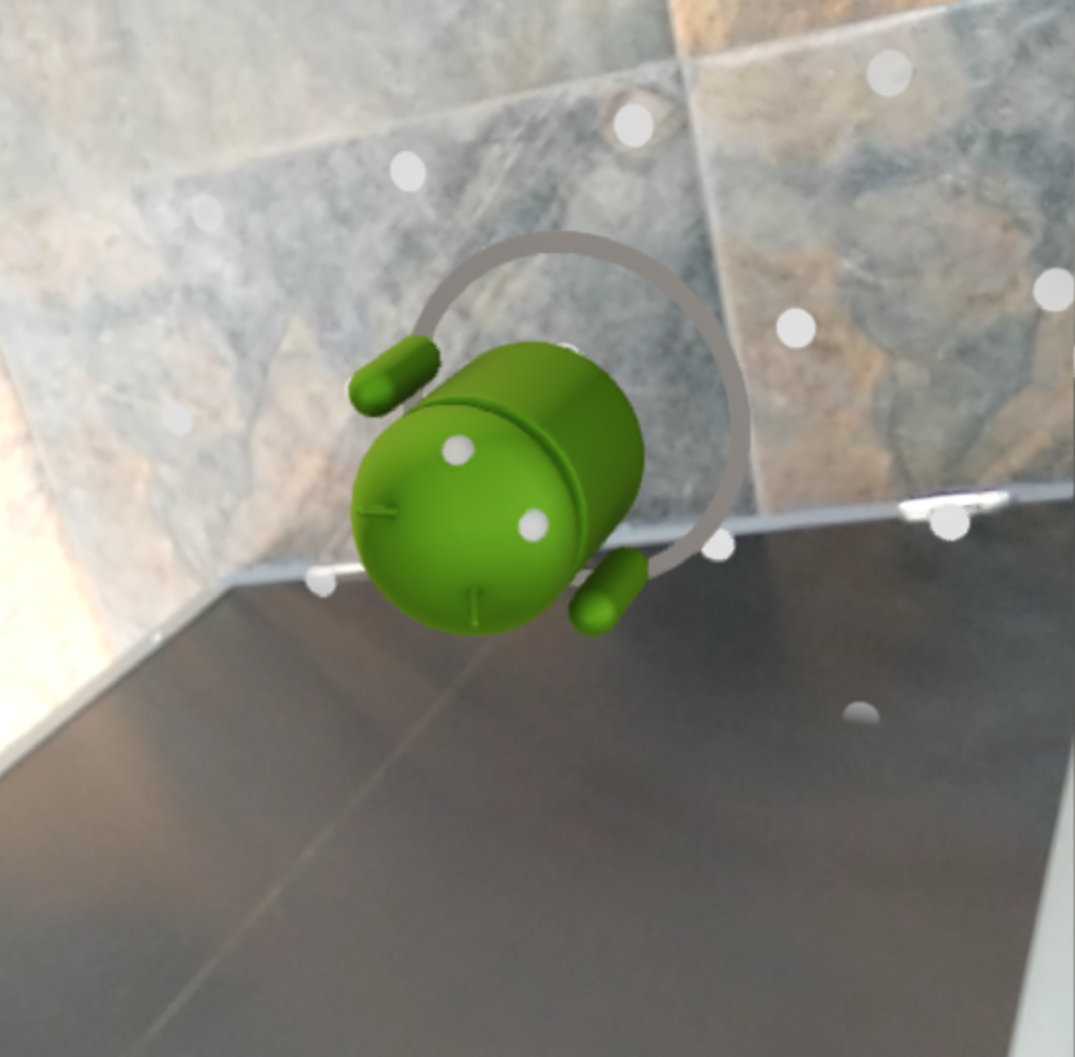
\includegraphics[width=8cm]{desarrollo/secciones/pruebas/motog6/img/SUPERFICIENEGRA.png}
		\caption{Malla de puntos no detectada en superficie negra}
		\label{fig:motog6supnegra}
	\end{minipage}\hfill
	\begin{minipage}{0.48\textwidth}
		\centering
		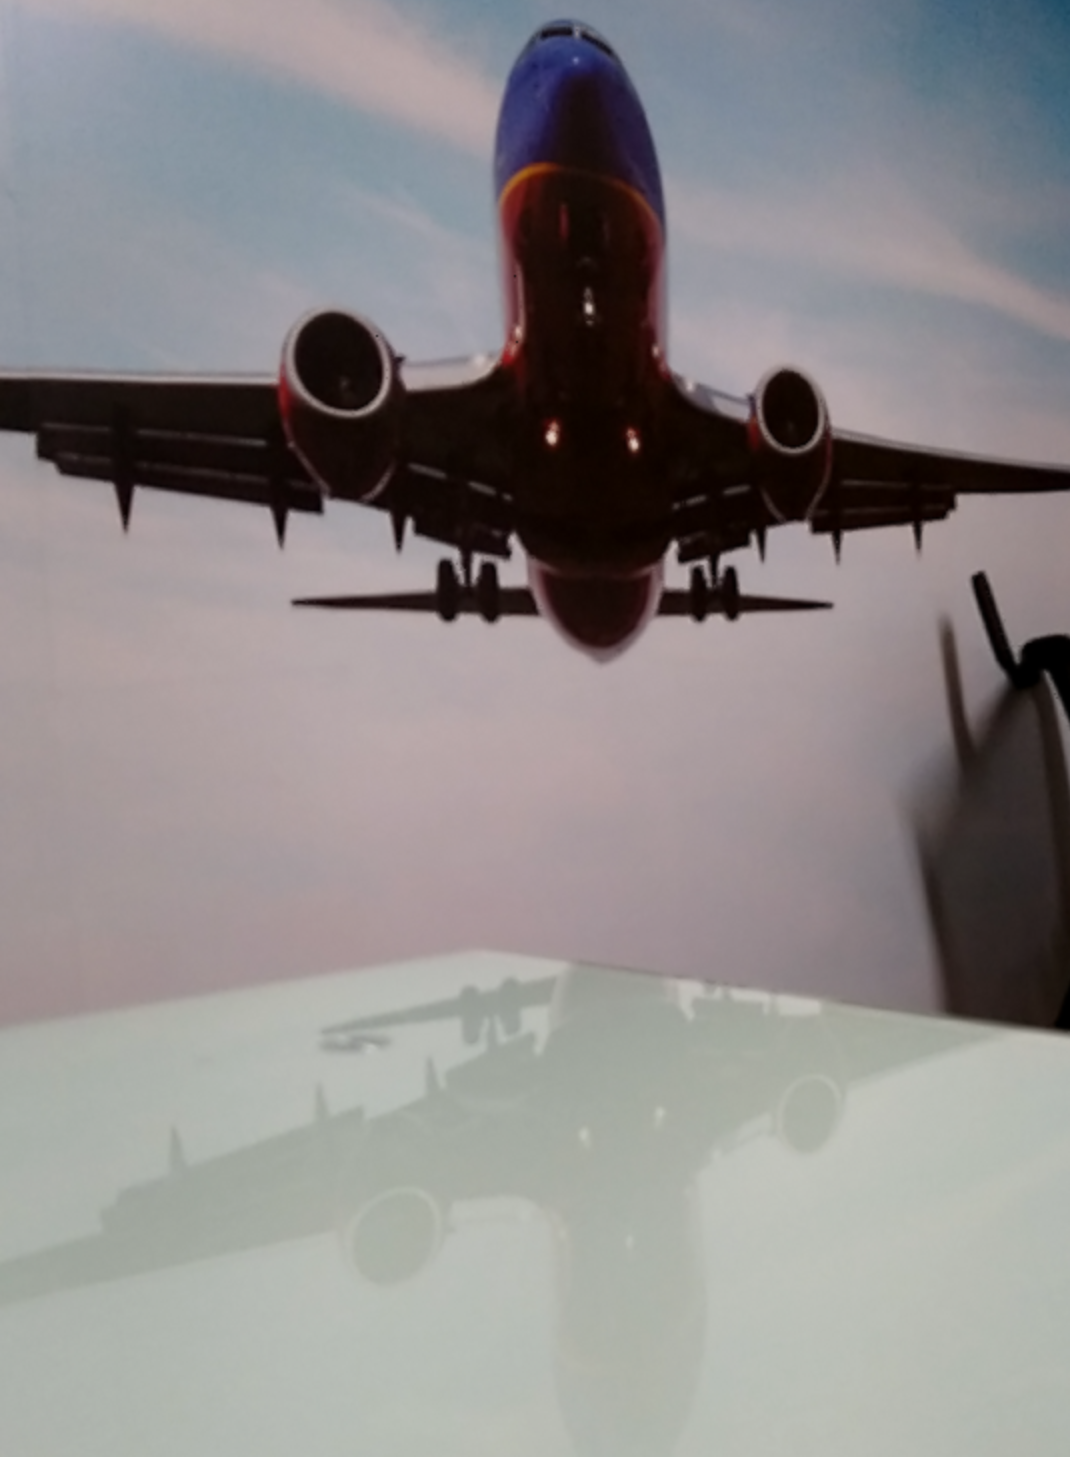
\includegraphics[width=6cm]{desarrollo/secciones/pruebas/motog6/img/VIDRIO.png}
		\caption{Malla de puntos no detectada en vidrio}
		\label{fig:motog6vidrio}
	\end{minipage}\hfill
\end{figure}

\textbf{\\Memoria de objetos} \par
Tras perder el enfoque de la cámara, al volverlo a tener, todos los objetos virtuales se volvieron a mostrar en el entorno virtual en la misma posición en la que habían sido puestos.

\textbf{Capacidad máxima de objetos} \par
Se colocaron 100 objetos virtuales en escena sin que la aplicación perdiera rendimiento. Todo funcionaba con total fluidez.

\begin{figure}[H]
	\begin{minipage}{0.48\textwidth}
		\centering
		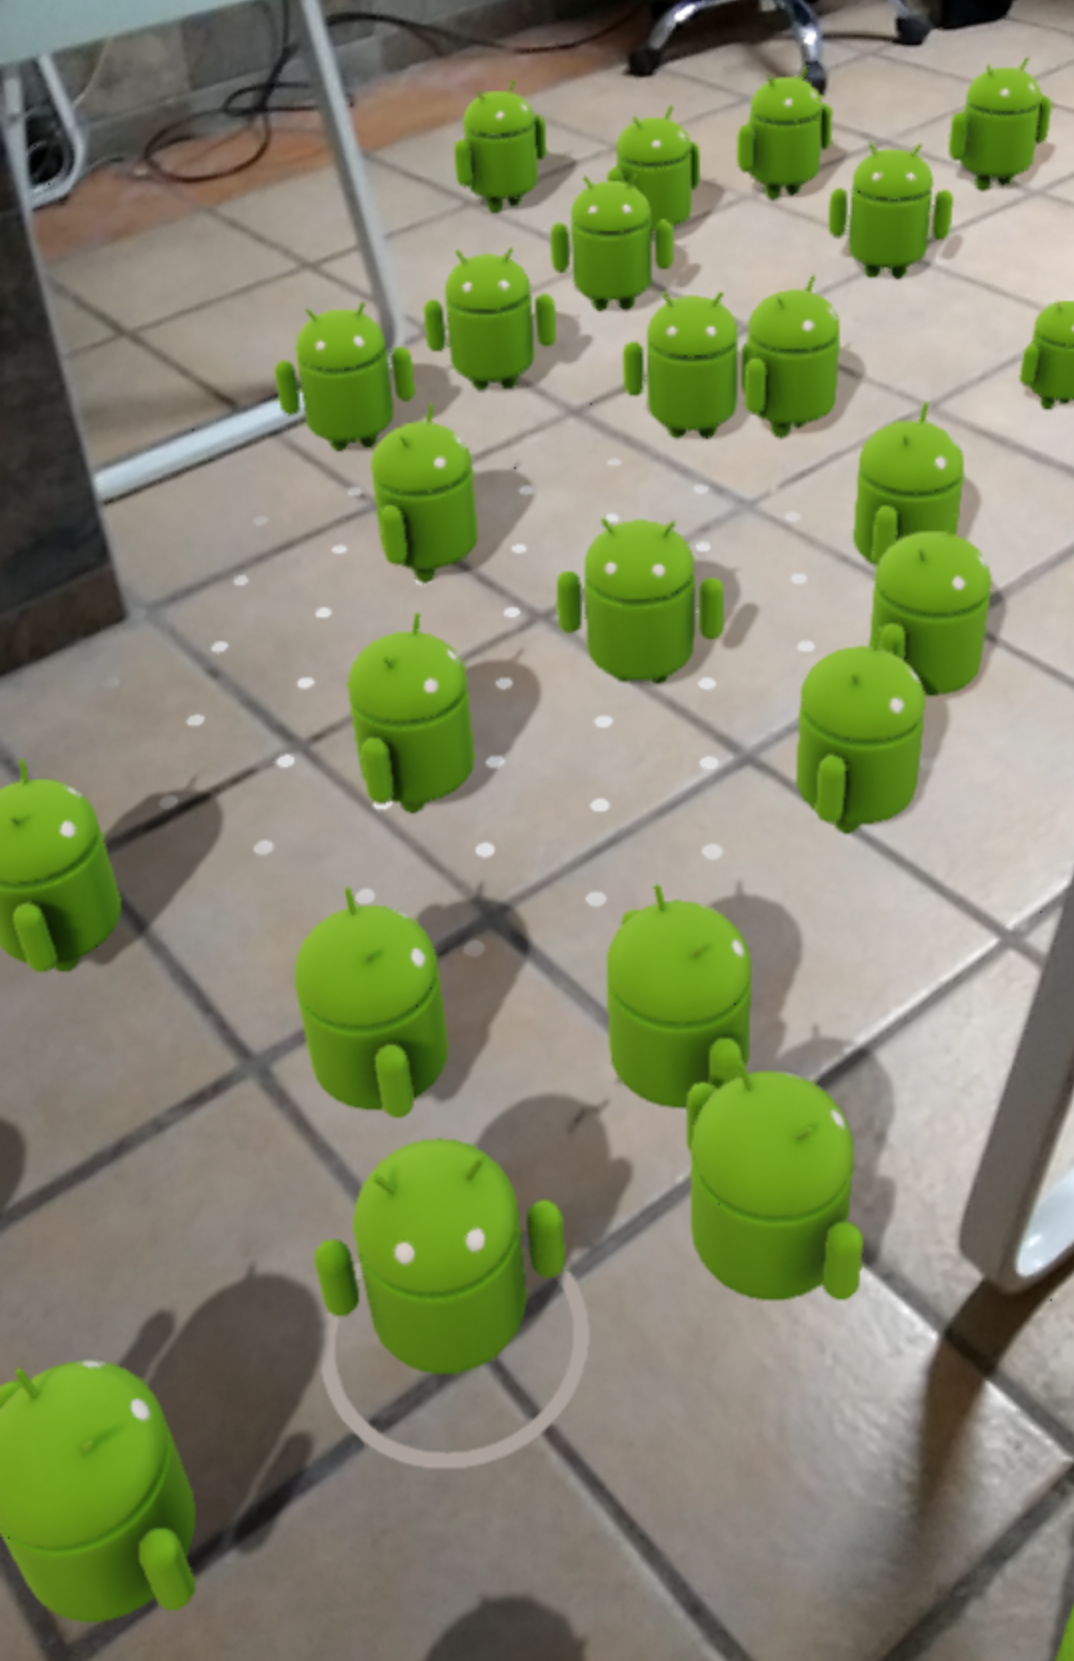
\includegraphics[width=5cm]{desarrollo/secciones/pruebas/motog6/img/CANTIDAD.png}
		\caption{Gran cantidad de objetos en escena}
		\label{fig:motog6escena}
	\end{minipage}\hfill
	\begin{minipage}{0.48\textwidth}
		
		\centering
		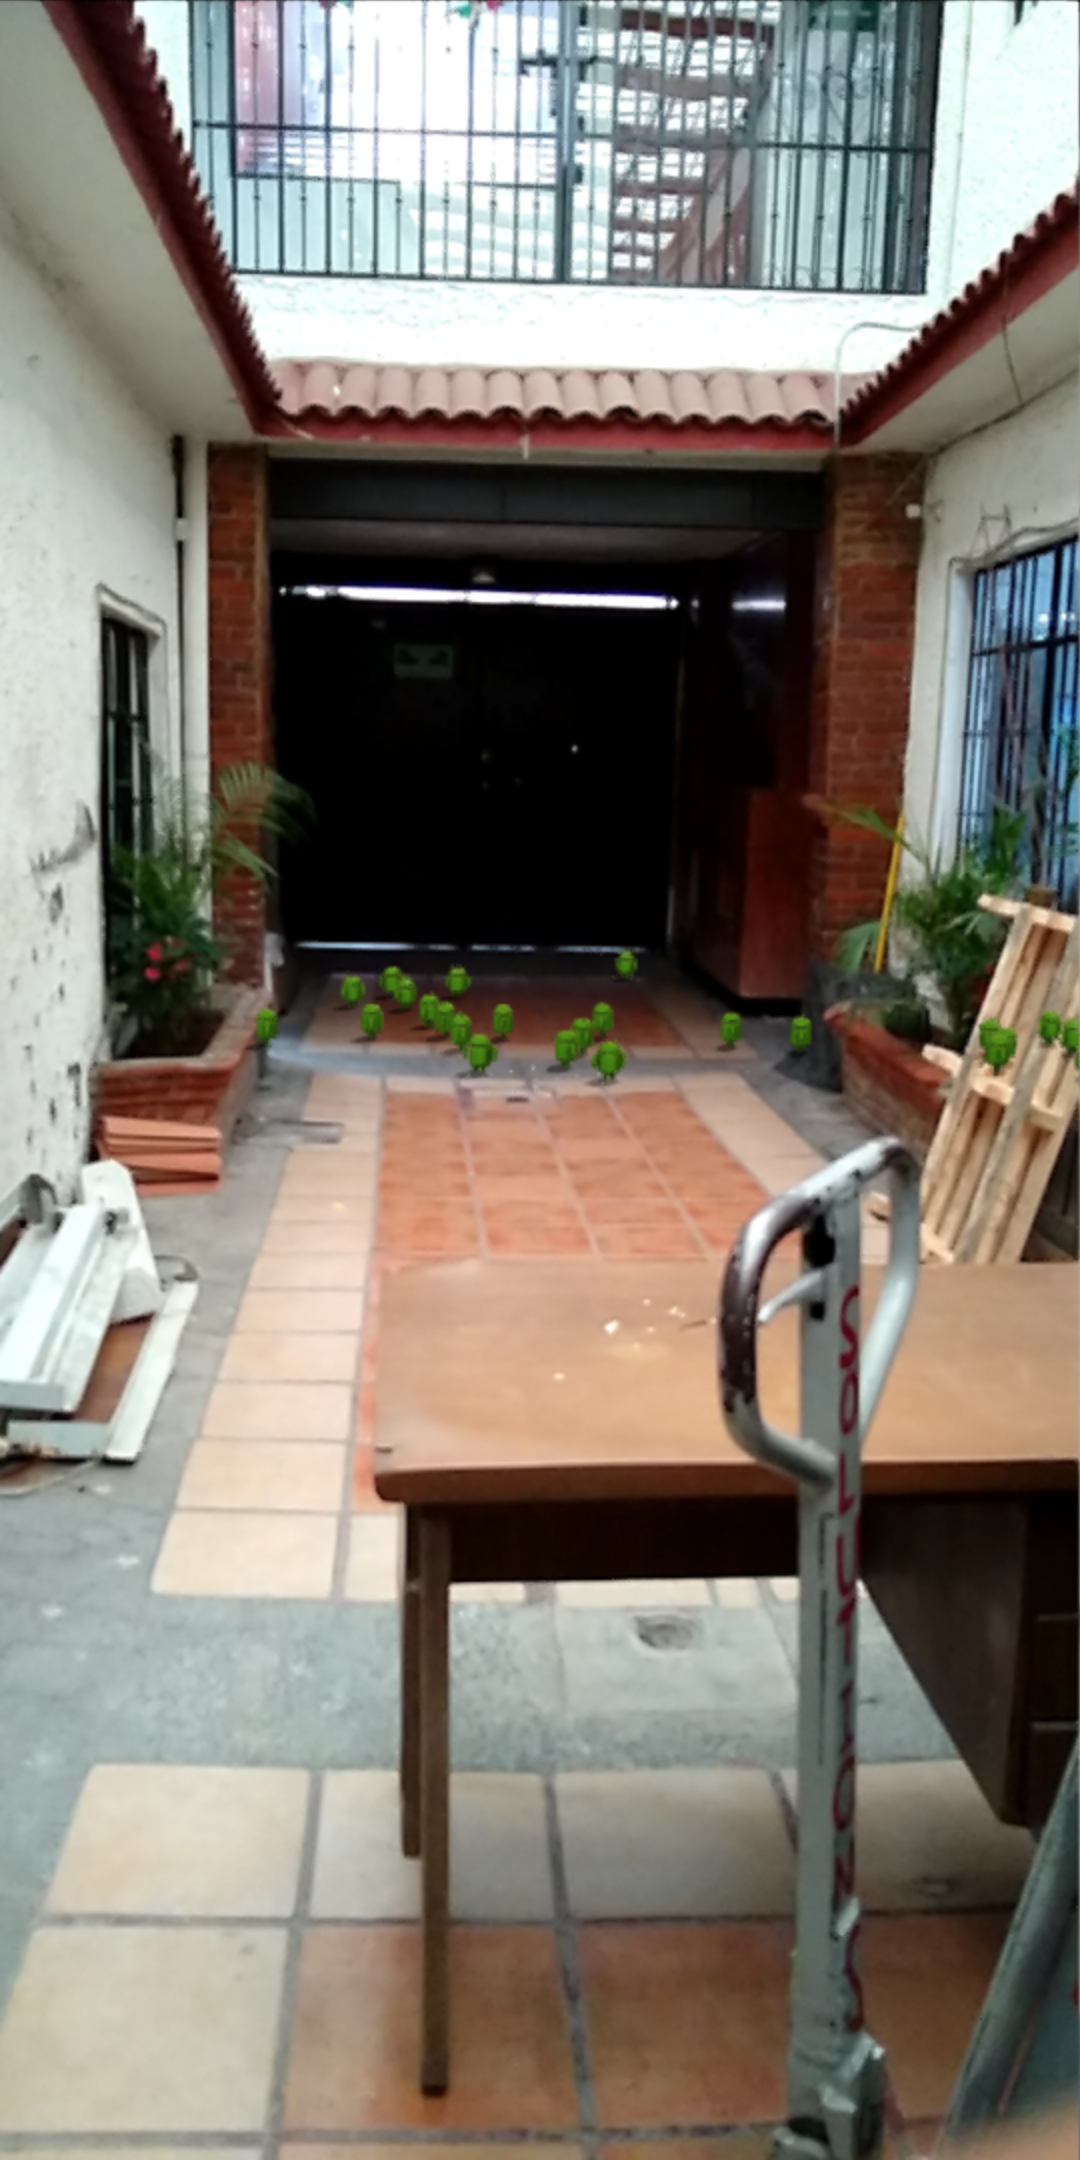
\includegraphics[width=5cm]{desarrollo/secciones/pruebas/motog6/img/DISTANCIA.png}
		\caption{Objetos puestos a gran distancia}
		\label{fig:motog6edistancia}
	\end{minipage}\hfill
\end{figure}

\textbf{Distancia} \par
Se colocó un objeto, después la cámara fue alejada hasta una distancia de \textbf{11.22m.} A esa distancia los objetos comenzaron a verse pixeleados, además comenzaron a desaparecer y reaparecer de forma intermitente.


\noindent
\subsubsection{ARcore}
\begin{table}[H]
	\centering
	\begin{tabular}{|c|c|}
		\hline
		\multicolumn{2}{|c|}{Especificaciones de prueba}   \\ \hline
		\textbf{DISPOSITIVO}              & Moto G6 XT1925 \\ \hline
		\textbf{FECHA}                    & 2018/08/25     \\ \hline
		\textbf{VERSIÓN DE SCENEFORM SDK} & V1.4.0         \\ \hline
		\textbf{VERSIÓN DE ARCORE SDK}    & V1.4.0         \\ \hline
		\textbf{VERSIÓN DE ANDROID}       & V8.0.0 (Oreo)  \\ \hline
	\end{tabular}
	\captionsetup{justification=centering}
	\caption{Especificaciones de prueba Arcore en Moto G6}
\end{table}

\textbf{Posición cardinal} \par
El objeto virtual se pudo apreciar con claridad desde los cuatro puntos cardinales y la vista superior. El ángulo de visualización del objeto al mover la cámara cambiaba a la perfección, dando una buena percepción de realismo.

%%IMAGENES DE PUNTOS CARDINALES
\begin{figure}[!htbp]
	\begin{minipage}{0.48\textwidth}
	\centering
		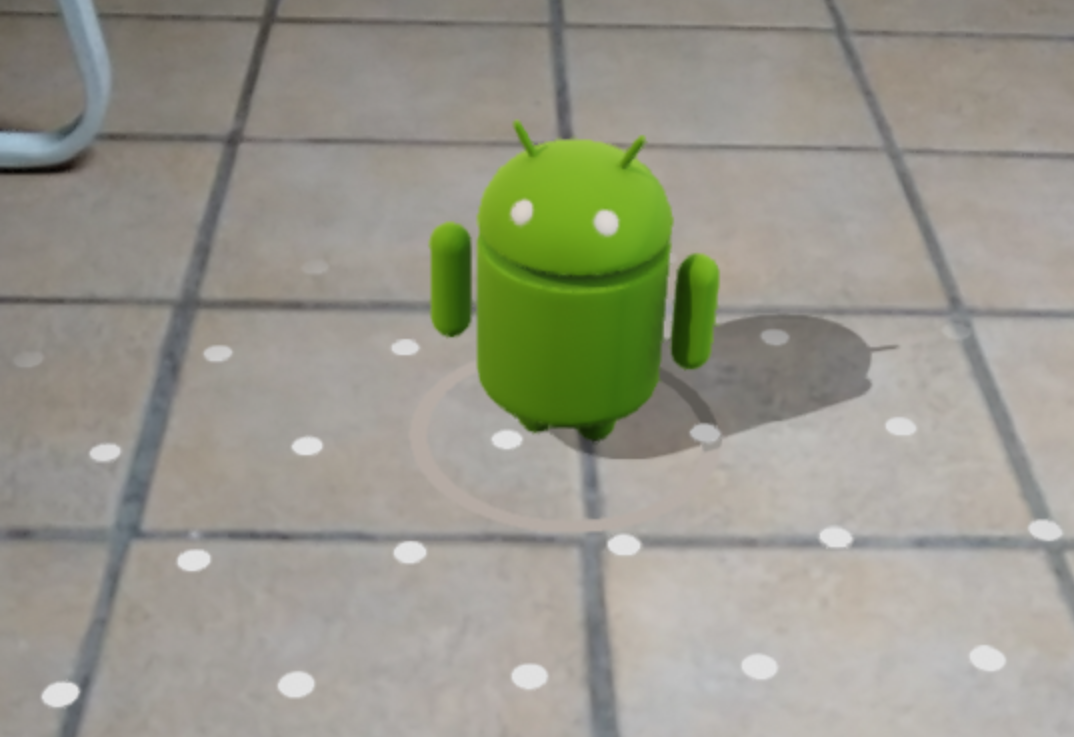
\includegraphics[width=8cm]{desarrollo/secciones/pruebas/motog6/img/NORTE.png}
		\caption{Posición Norte}
		\label{fig:motog6norte}
	\end{minipage}\hfill
	\begin{minipage}{0.48\textwidth}
	\centering
	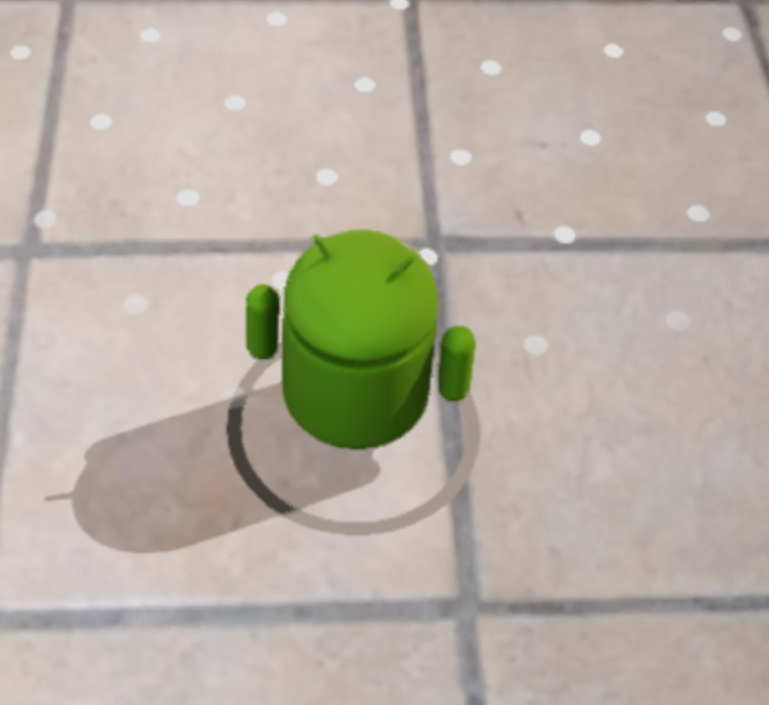
\includegraphics[width=8cm]{desarrollo/secciones/pruebas/motog6/img/SUR.png}
	\caption{Posición Sur}
	\label{fig:motog6sur}
	\end{minipage}\hfill
\end{figure}

\begin{figure}[!htbp]
	\begin{minipage}{0.48\textwidth}
		\centering
		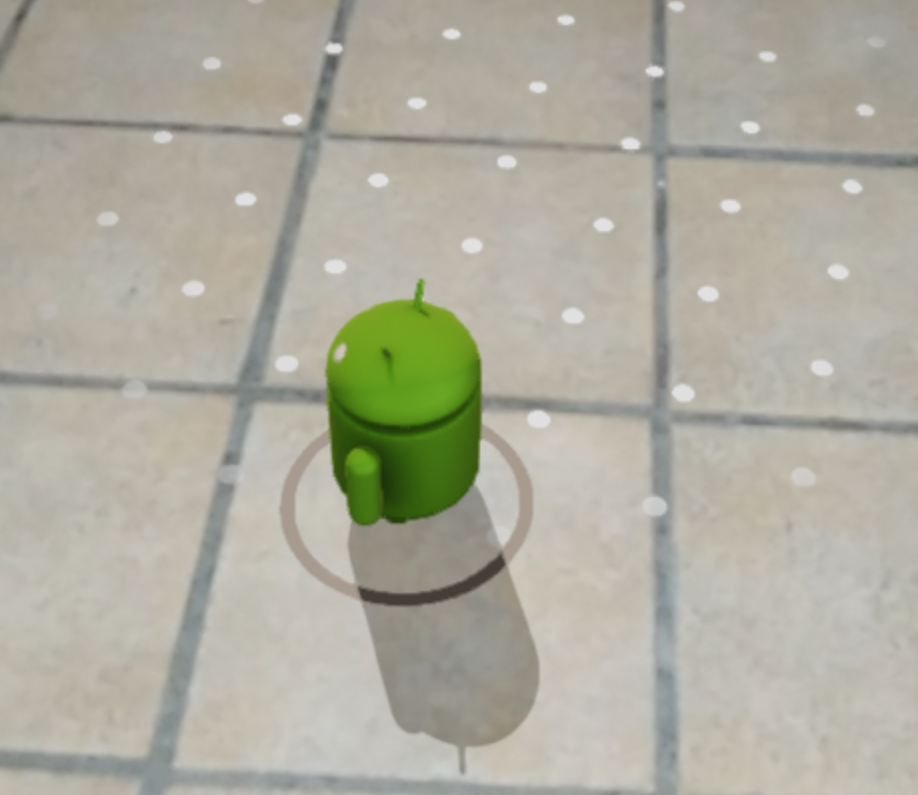
\includegraphics[width=8cm]{desarrollo/secciones/pruebas/motog6/img/ESTE.png}
		\caption{Posición Este}
		\label{fig:motog6norte}
	\end{minipage}\hfill
	\begin{minipage}{0.48\textwidth}
		\centering
		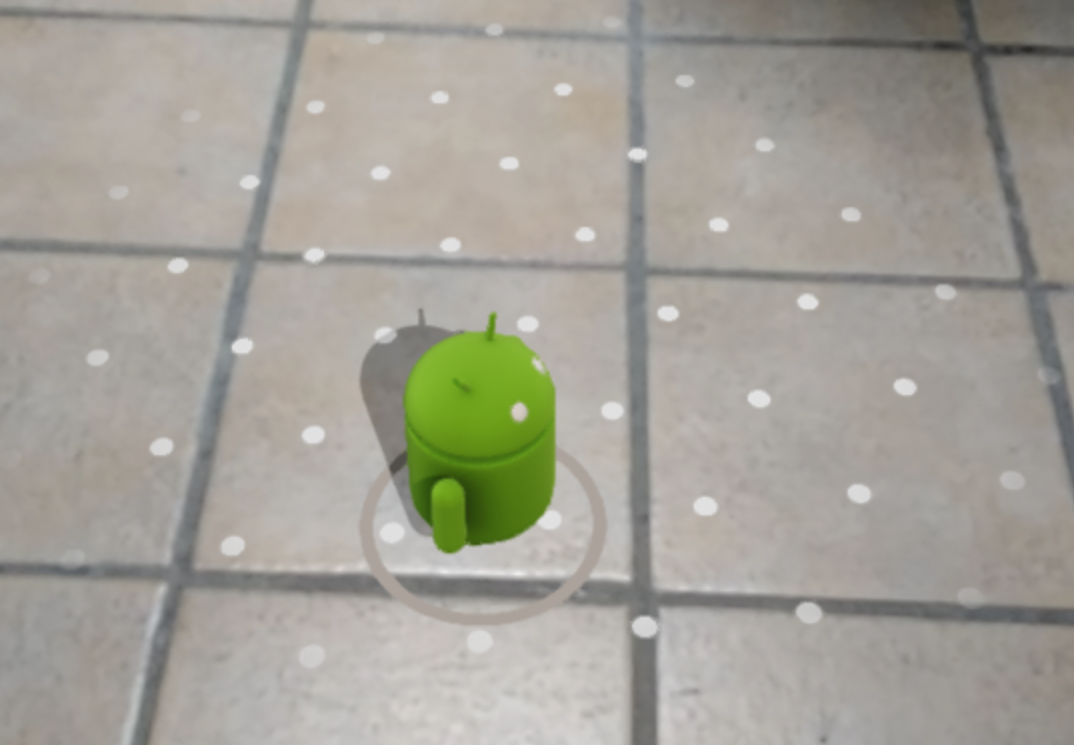
\includegraphics[width=8cm]{desarrollo/secciones/pruebas/motog6/img/OESTE.png}
		\caption{Posición Oeste}
		\label{fig:motog6oeste}
	\end{minipage}\hfill
\end{figure}

\textbf{Tamaño relativo} \par
Al acercar o alejar la cámara el objeto virtual variaba su tamaño de forma adecuada, como si el objeto realmente estuviera en la posición donde fue superpuesto.


\begin{figure}[!htbp]
	\begin{minipage}{0.48\textwidth}
		\centering
		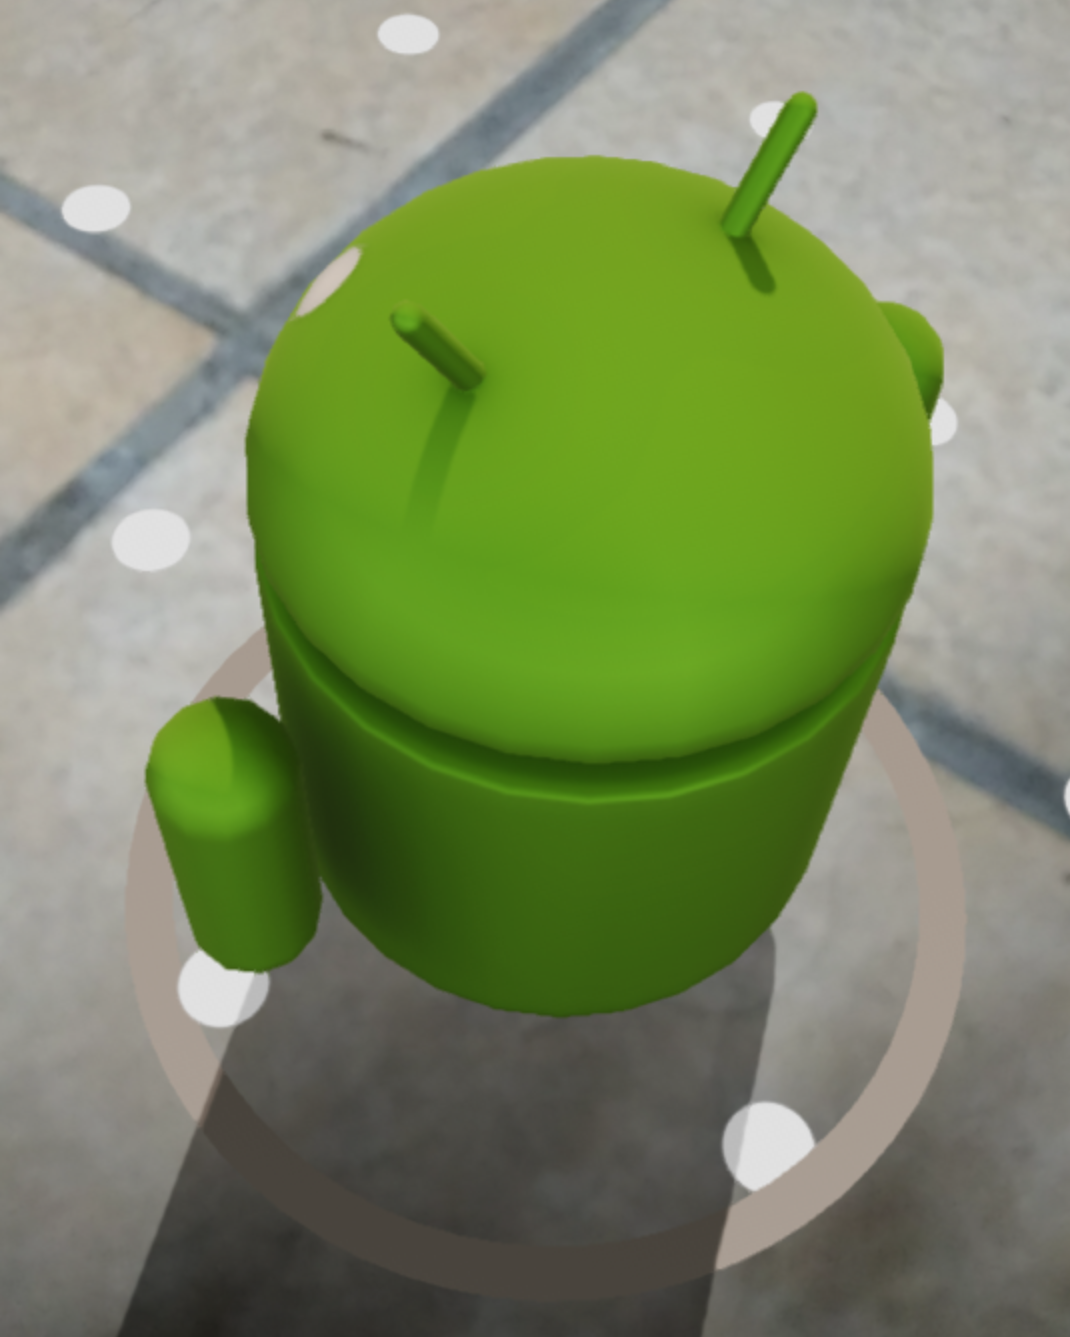
\includegraphics[width=8cm]{desarrollo/secciones/pruebas/motog6/img/CERCA.png}
		\caption{Objeto visto de cerca}
		\label{fig:motog6cerca}
	\end{minipage}\hfill
	\begin{minipage}{0.48\textwidth}
		\centering
		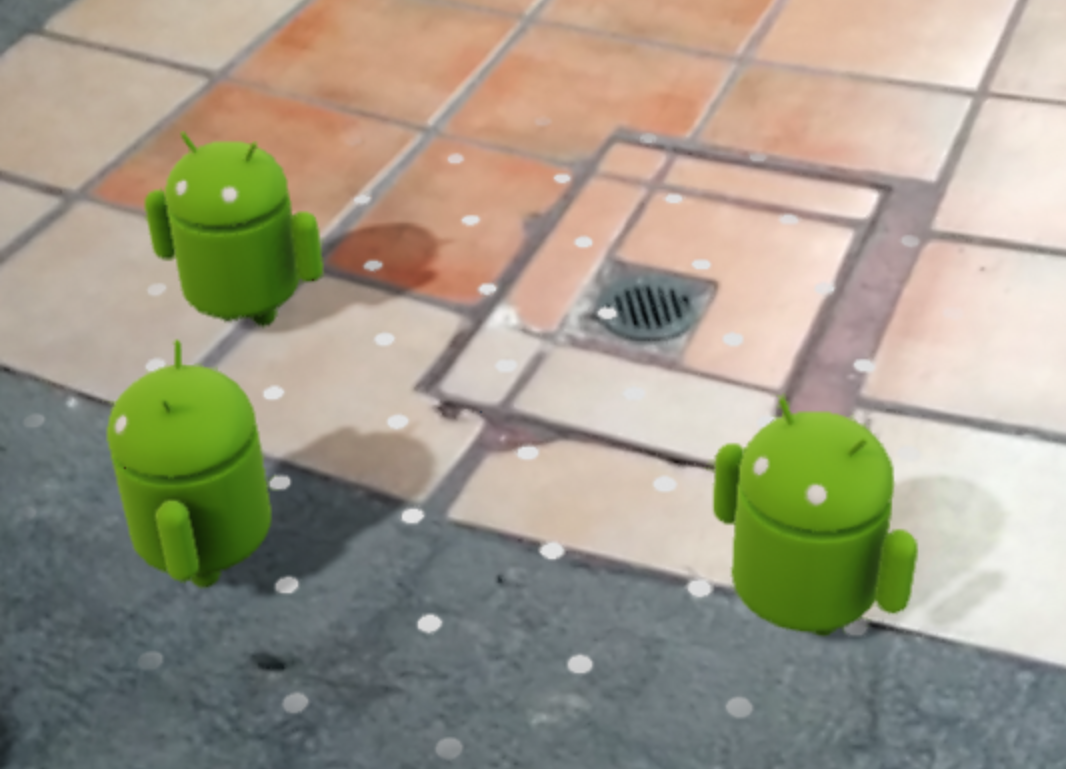
\includegraphics[width=8cm]{desarrollo/secciones/pruebas/motog6/img/LUZALTA.png}
		\caption{Luz alta}
		\label{fig:motog6lalta}
	\end{minipage}\hfill
\end{figure}

\textbf{Luminosidad} \par
Al poner el objeto virtual en entornos con diferente cantidad de luz, la cantidad de luz en el objeto virtual también variaba. En un entorno con ausencia casi total de luz el objeto apenas era perceptible, mientras que en un entorno con bastante luz, el objeto se veía altamente iluminado.

\begin{figure}[!htbp]
	\begin{minipage}{0.48\textwidth}
		\centering
		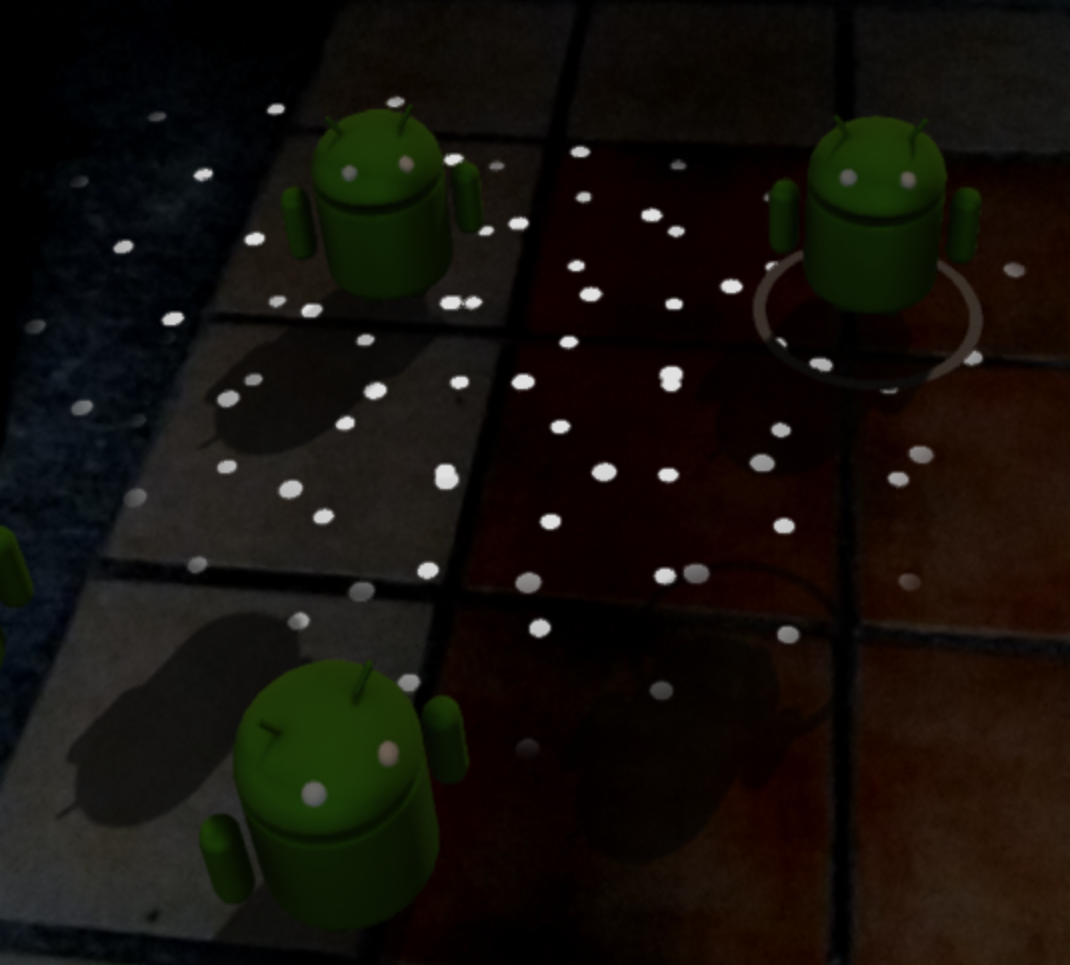
\includegraphics[width=8cm]{desarrollo/secciones/pruebas/motog6/img/LUZBAJA.png}
		\caption{Luz baja}
		\label{fig:motog6lbaja}
	\end{minipage}\hfill
	\begin{minipage}{0.48\textwidth}
		\centering
		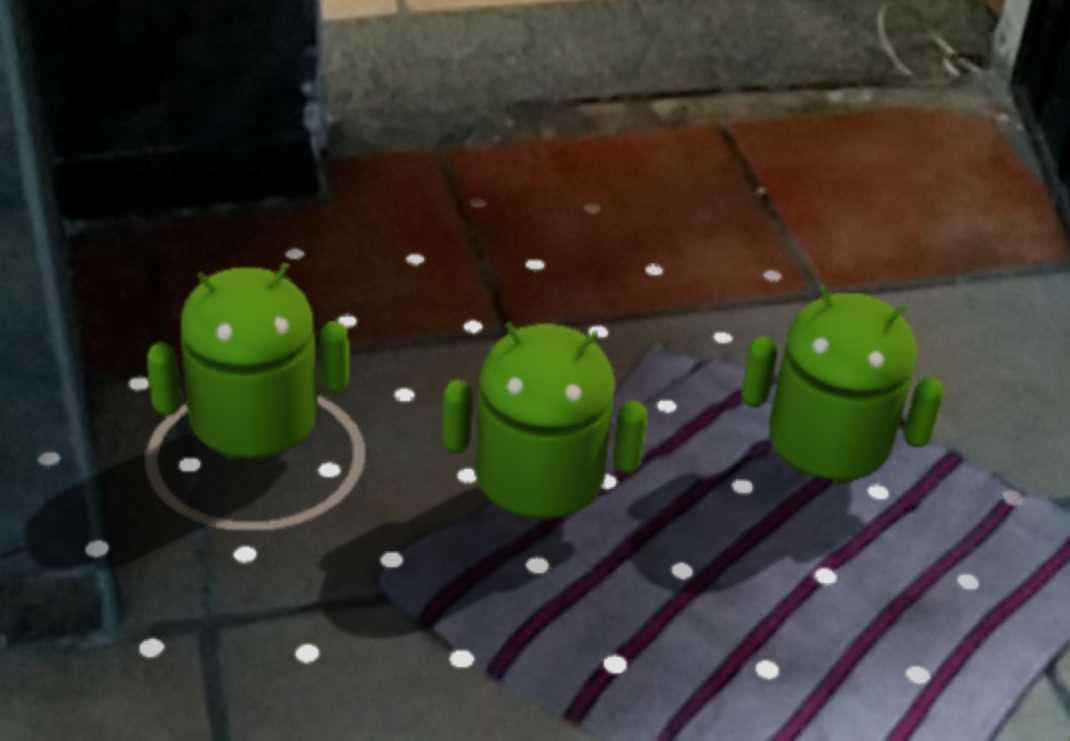
\includegraphics[width=8cm]{desarrollo/secciones/pruebas/motog6/img/LUZMEDIA.png}
		\caption{Luz media}
		\label{fig:motog6lmedia}
	\end{minipage}\hfill
\end{figure}

\textbf{Superficie} \par
Se probó posicionar el objeto virtual en cuatro superficies: concreto gris, concreto blanco, azulejo y vidrio.\par
Concreto gris.- El objeto se pudo posicionar a la perfección.\par
Concreto blanca.- El objeto no se pudo posicionar. La maya de puntos ni si quiera era detectada en ésta superficie debido a la ausencia de texturas.\par
Azulejo.- El objeto se pudo posicionar a la perfección.\par
Vidrio.- El objeto no pudo ser posicionado en ésta superficie debido a las propiedades reflejantes que posee.\par

\begin{figure}[!htbp]
	\begin{minipage}{0.48\textwidth}
		\centering
		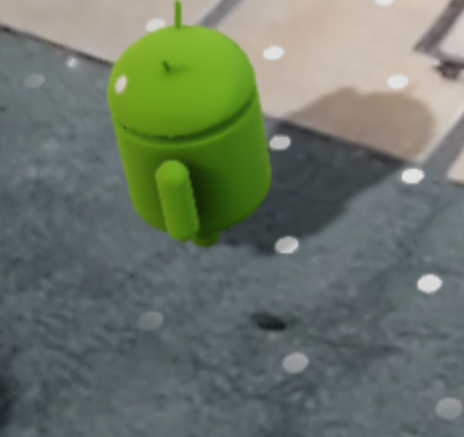
\includegraphics[width=8cm]{desarrollo/secciones/pruebas/motog6/img/CONCRETO.png}
		\caption{Objeto colocado en concreto}
		\label{fig:motog6concreto}
	\end{minipage}\hfill
	\begin{minipage}{0.48\textwidth}
		\centering
		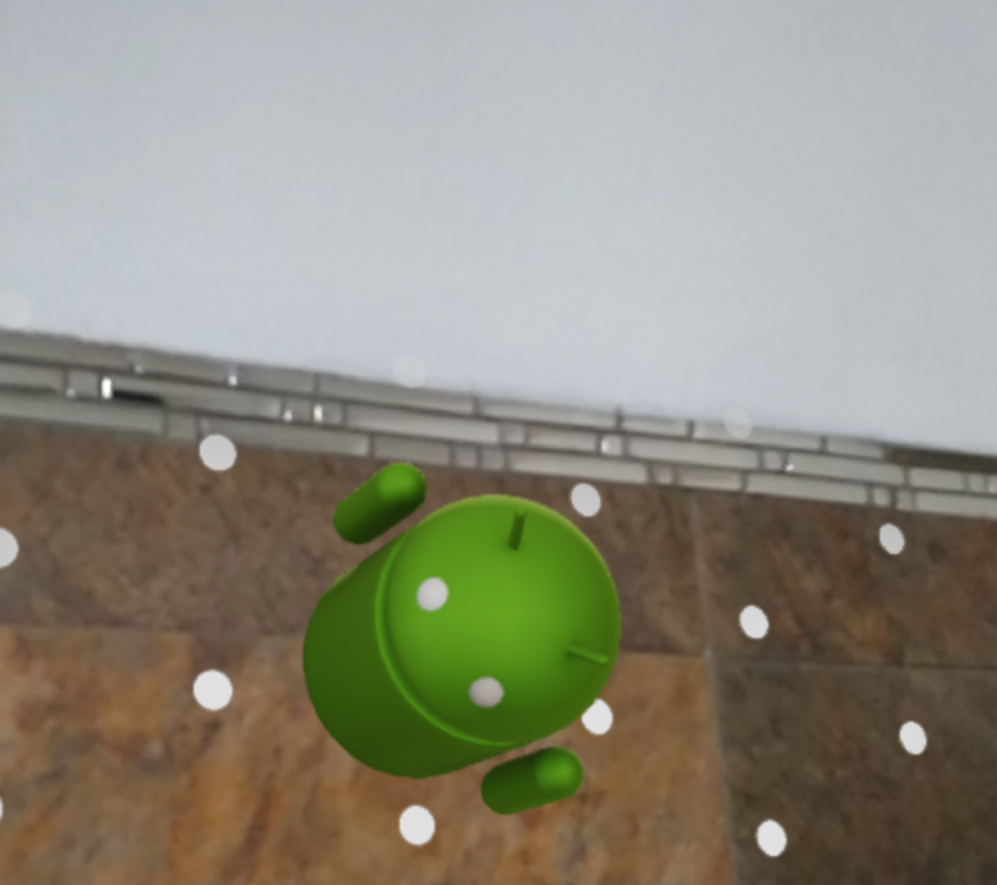
\includegraphics[width=8cm]{desarrollo/secciones/pruebas/motog6/img/SUPBLANCA.png}
		\caption{Objeto colocado en superficie blanca}
		\label{fig:motog6supblanca}
	\end{minipage}\hfill
\end{figure}

\begin{figure}[H]
	\begin{minipage}{0.48\textwidth}
		\centering
		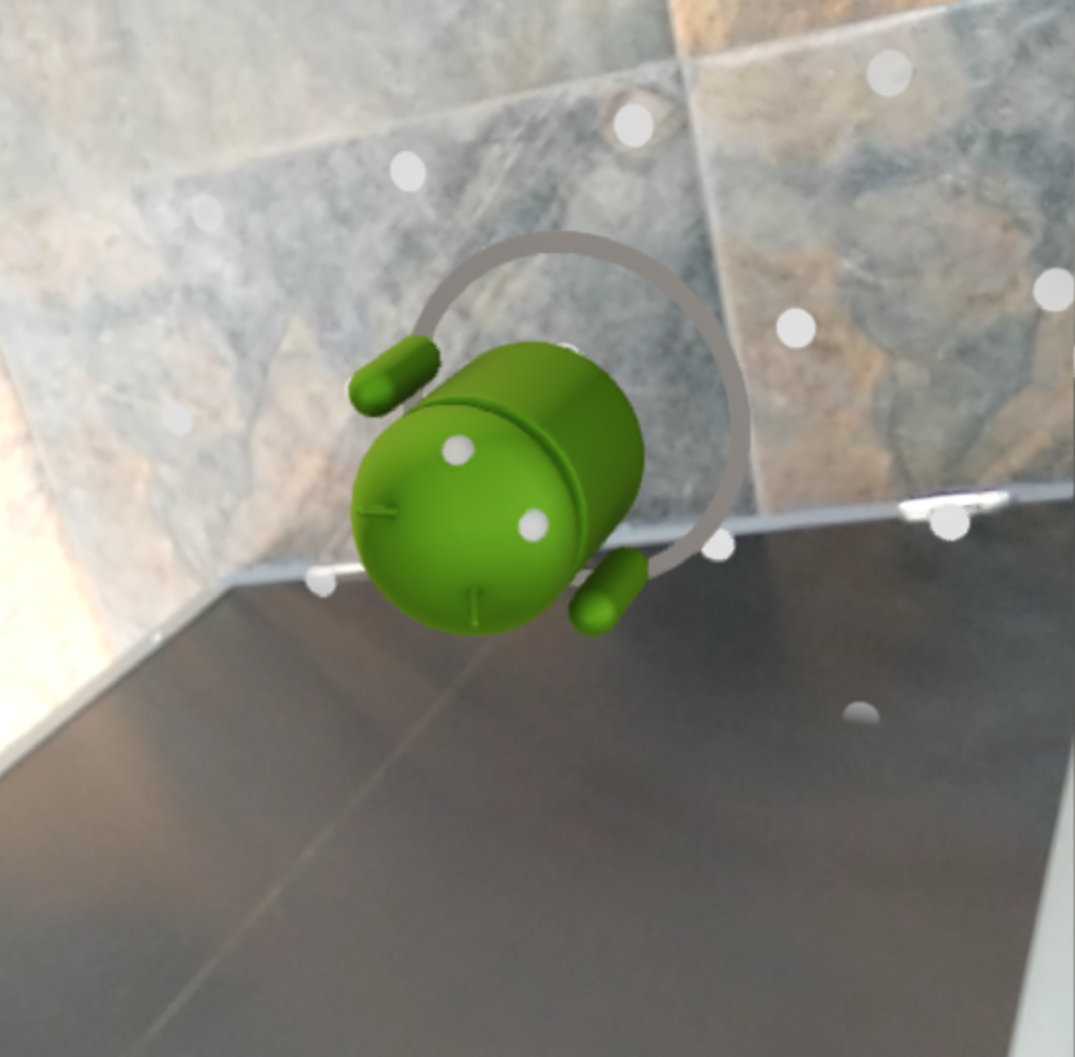
\includegraphics[width=8cm]{desarrollo/secciones/pruebas/motog6/img/SUPERFICIENEGRA.png}
		\caption{Malla de puntos no detectada en superficie negra}
		\label{fig:motog6supnegra}
	\end{minipage}\hfill
	\begin{minipage}{0.48\textwidth}
		\centering
		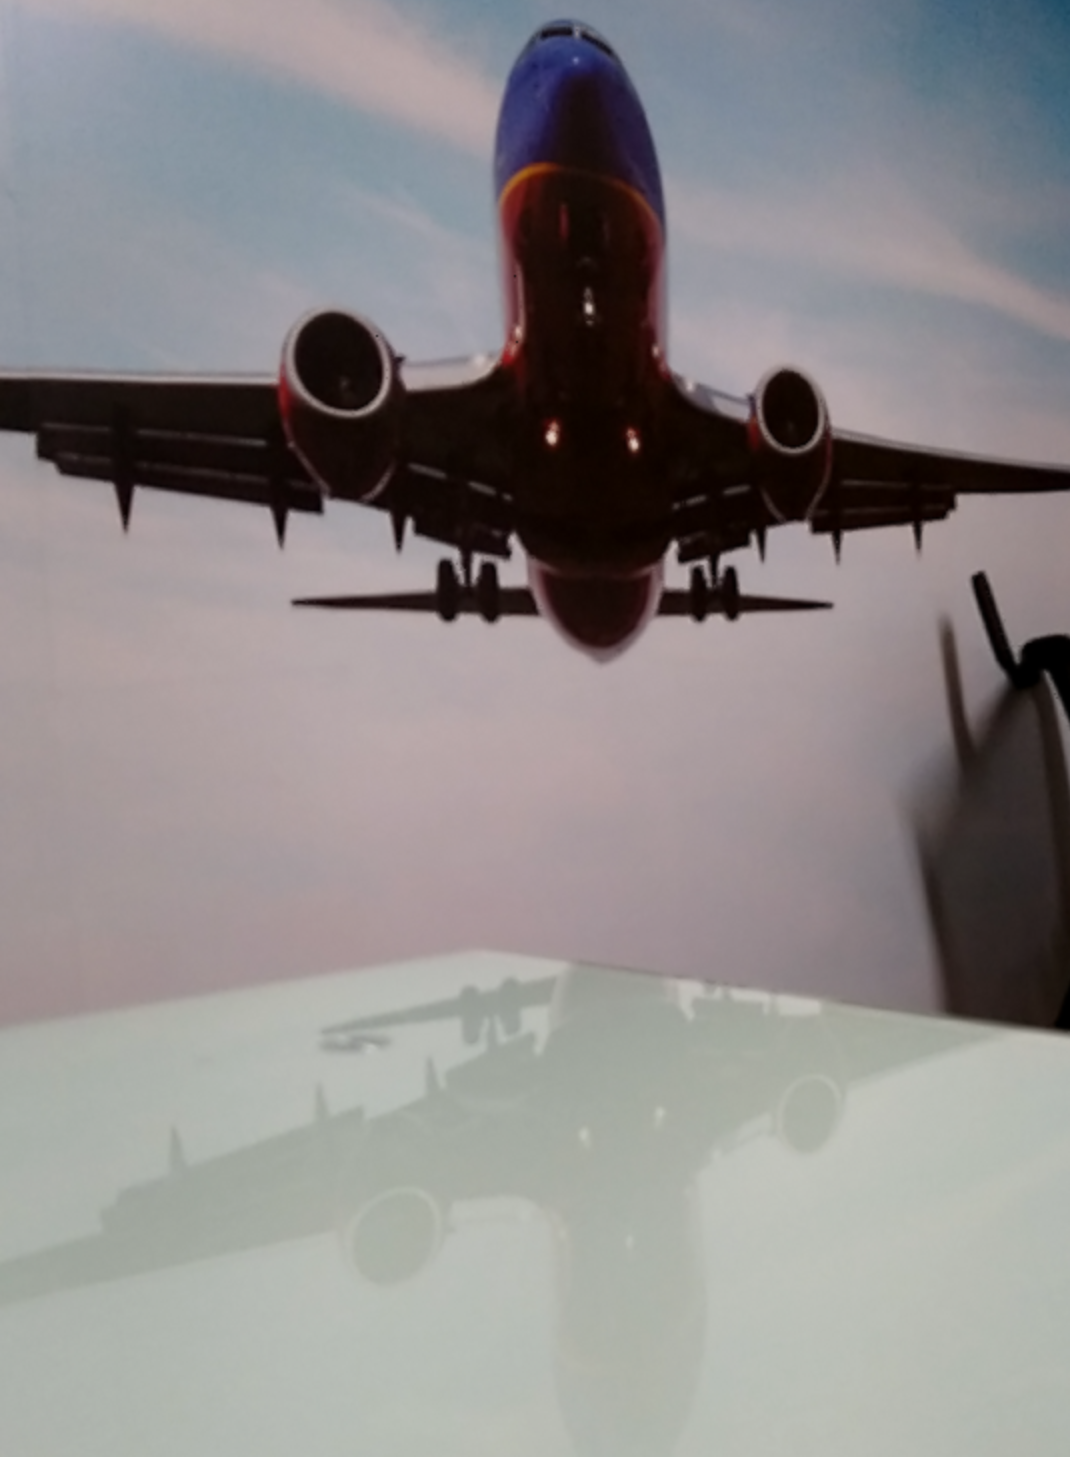
\includegraphics[width=6cm]{desarrollo/secciones/pruebas/motog6/img/VIDRIO.png}
		\caption{Malla de puntos no detectada en vidrio}
		\label{fig:motog6vidrio}
	\end{minipage}\hfill
\end{figure}

\textbf{\\Memoria de objetos} \par
Tras perder el enfoque de la cámara, al volverlo a tener, todos los objetos virtuales se volvieron a mostrar en el entorno virtual en la misma posición en la que habían sido puestos.

\textbf{Capacidad máxima de objetos} \par
Se colocaron 100 objetos virtuales en escena sin que la aplicación perdiera rendimiento. Todo funcionaba con total fluidez.

\begin{figure}[H]
	\begin{minipage}{0.48\textwidth}
		\centering
		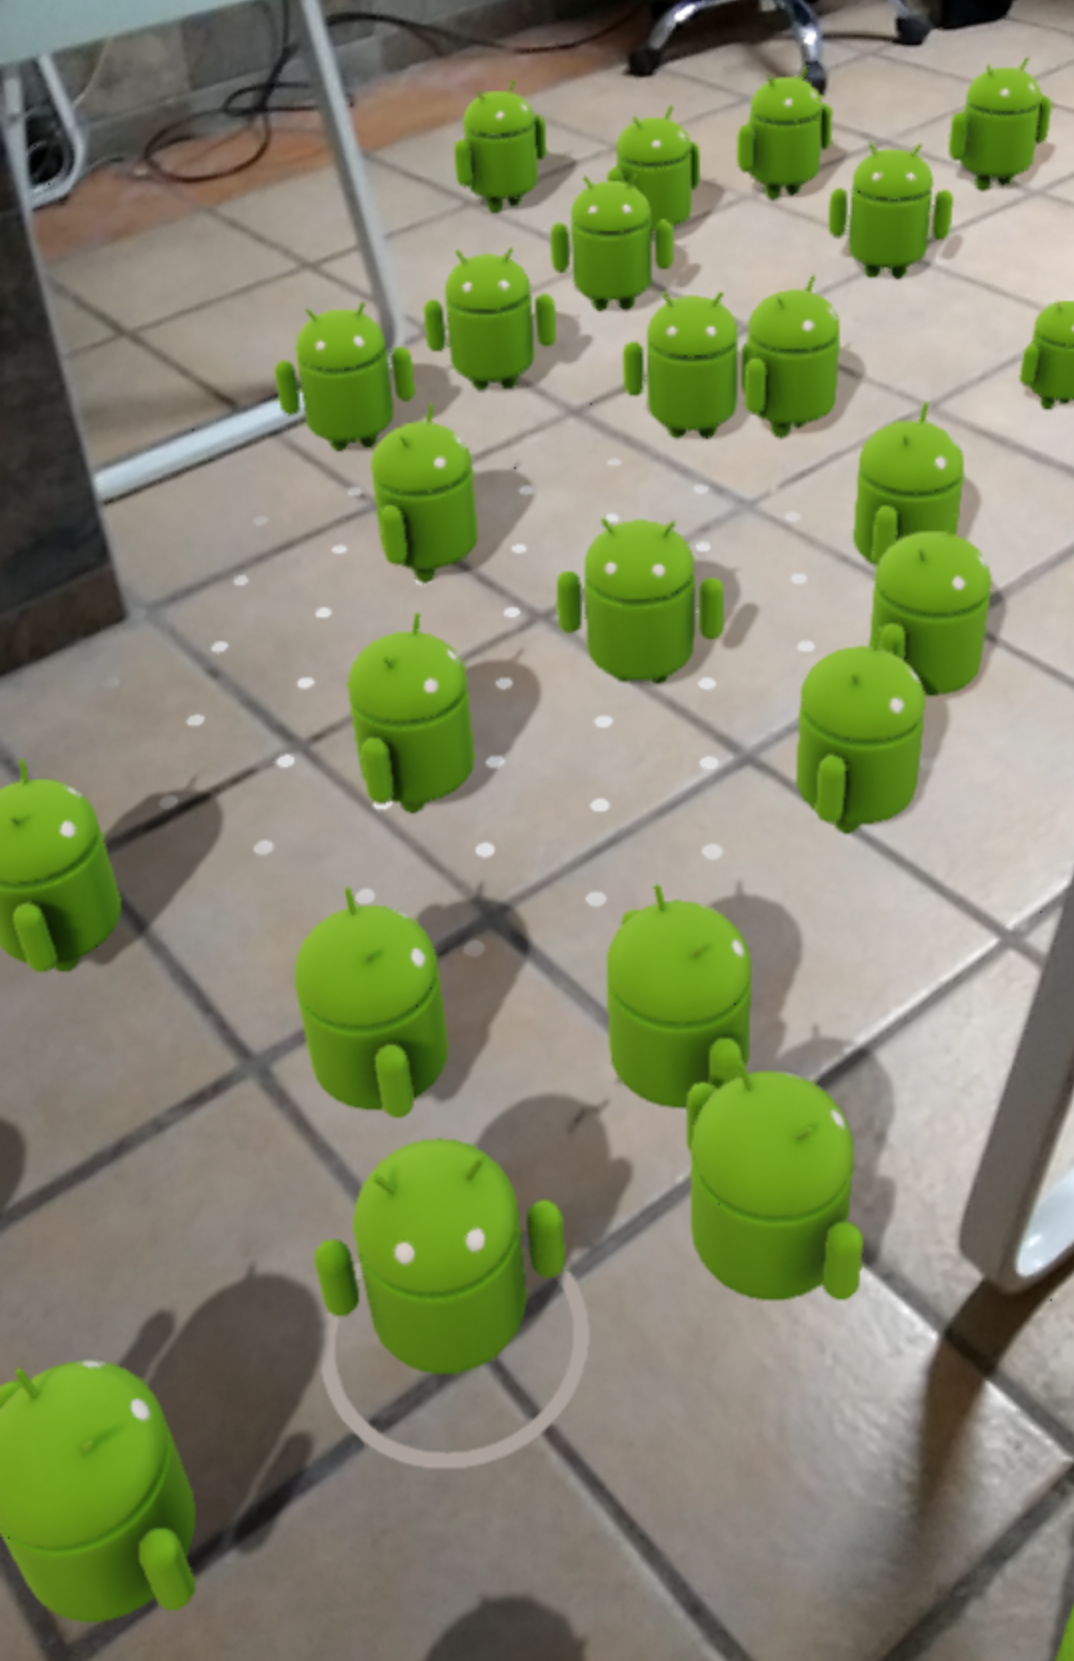
\includegraphics[width=5cm]{desarrollo/secciones/pruebas/motog6/img/CANTIDAD.png}
		\caption{Gran cantidad de objetos en escena}
		\label{fig:motog6escena}
	\end{minipage}\hfill
	\begin{minipage}{0.48\textwidth}
		
		\centering
		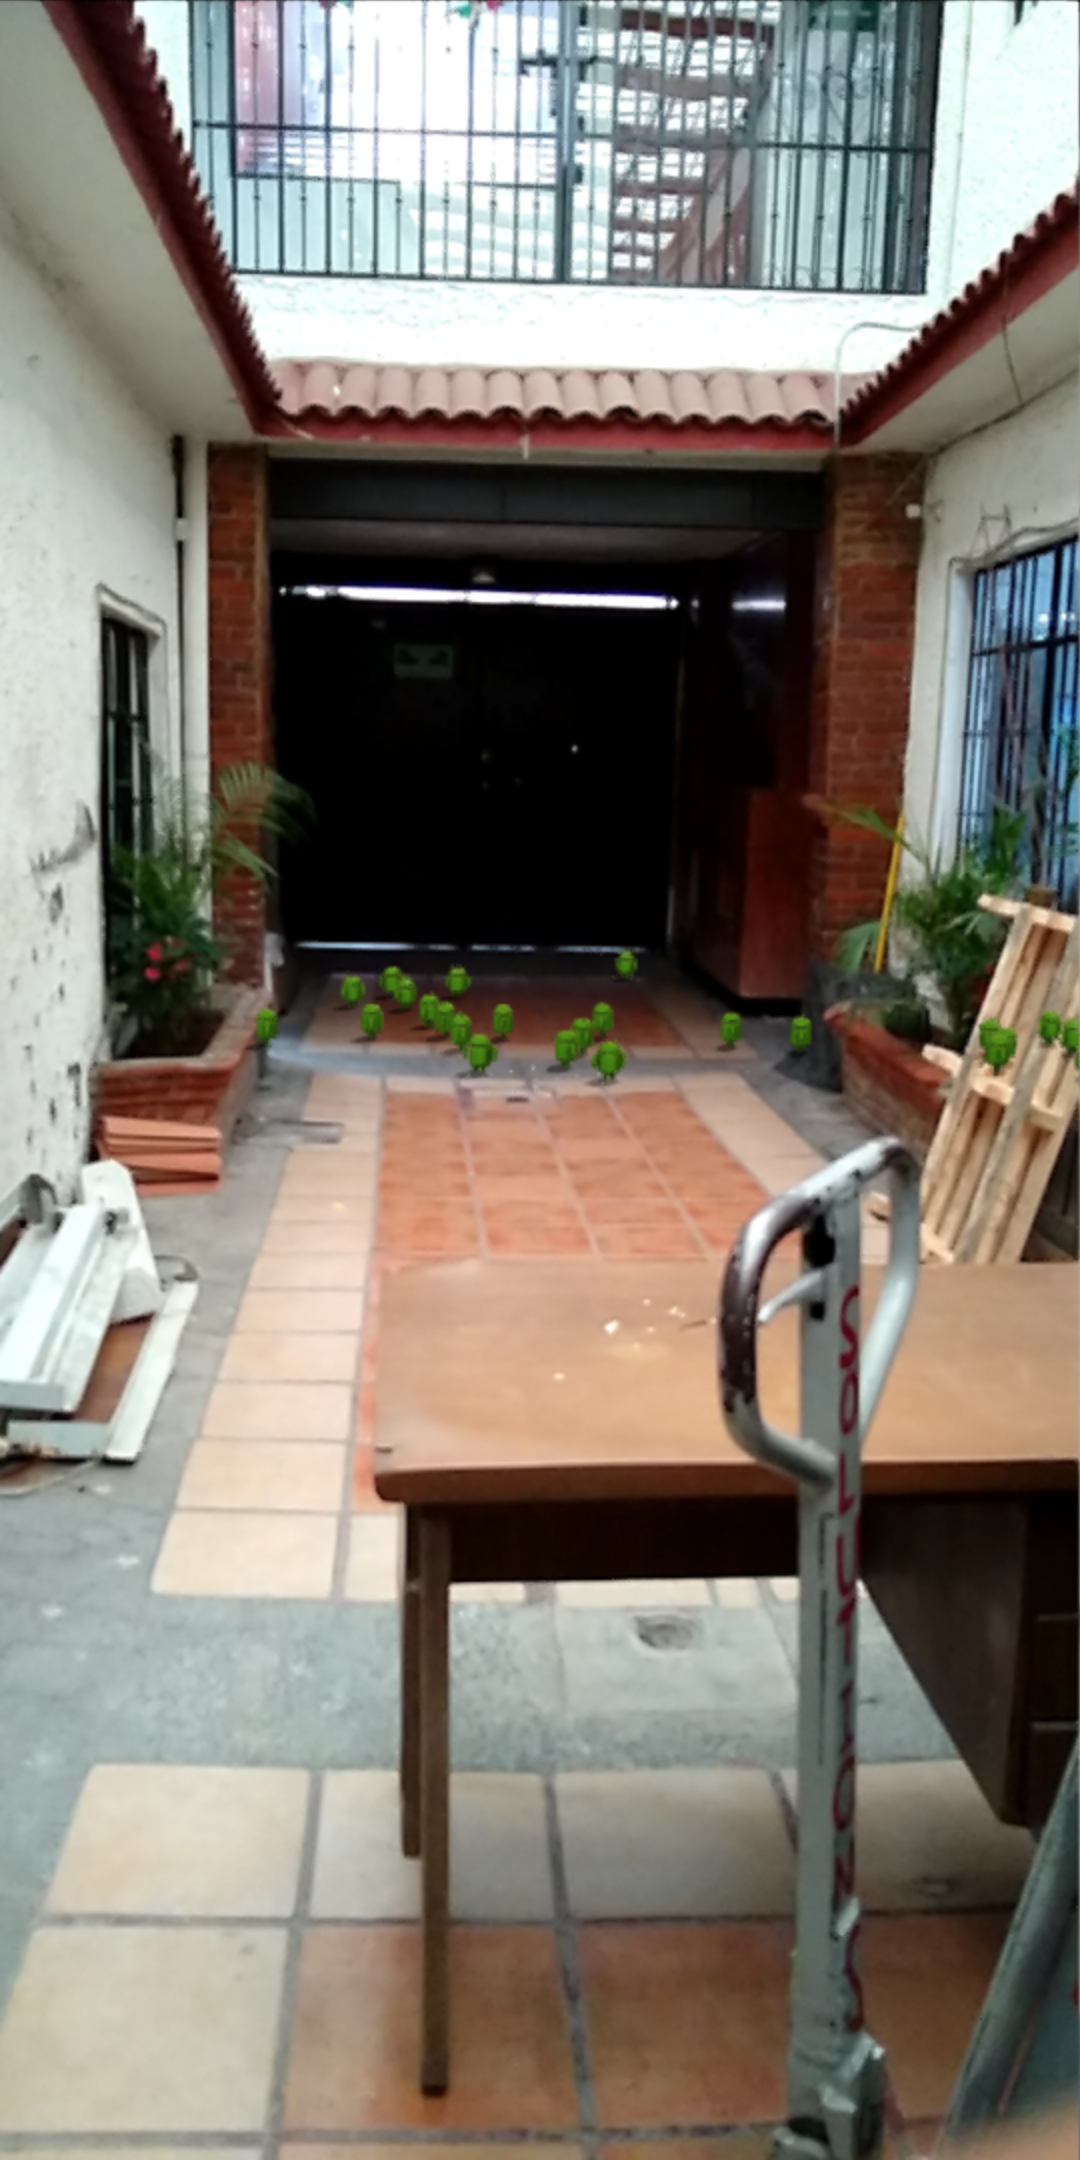
\includegraphics[width=5cm]{desarrollo/secciones/pruebas/motog6/img/DISTANCIA.png}
		\caption{Objetos puestos a gran distancia}
		\label{fig:motog6edistancia}
	\end{minipage}\hfill
\end{figure}

\textbf{Distancia} \par
Se colocó un objeto, después la cámara fue alejada hasta una distancia de \textbf{11.22m.} A esa distancia los objetos comenzaron a verse pixeleados, además comenzaron a desaparecer y reaparecer de forma intermitente.


\noindent

\subsubsection{Conclusión de pruebas de contexto}
Tras las pruebas de contexto realizadas con ARCore y Vuforia, se tomó la decisión de desarrollar el proyecto con ARCore por las siguientes razones:
\begin{itemize}
	\item Vuforia presentó intermitencia en las pruebas de posición cardinal.
	\item Vuforia depende de un marcador físico para posicionar el objeto.
	\item La dependencia de Vuforia al marcador físico elimina la capacidad de memoria de objetos.
	\item Vuforia en ambientes con luz muy baja es incapaz de funcionar.
	\item Con Vuforia se requieren imprimir tantos marcadores físicos como objetos se deseen visualizar. Es decir, si se quieren mostrar 30 muebles en escena, es necesario imprimir y posicionar los 30 marcadores en el entorno físico.
\end{itemize}
\newpage

\subsubsection{Establecimiento de interesados}
\textbf{Desarrolladores} \par
Para poder construir la aplicación requeriremos desarrolladores que puedan diseñar la arquitectura que tendrá la aplicación y programarla. Los tres desarrolladores que estarán trabajando en el proyecto son Gerardo Aramis Cabello Acosta, Martín Alejandro Carrillo Mendoza y Saúl del Pilar Morales. Su intervención se requerirá en todas las iteraciones del proyecto desde la I a la IX.\par
\textbf{Directores} \par
Los directores serán los encargados de supervisar los avances del proyecto en cada iteración. También serán elementos de apoyo a los que los desarrolladores podrán acudir en caso de tener alguna duda o complicación. Su intervención se requerirá durante todo el desarrollo del proyecto desde la iteración I a la iteración IX.\par
\textbf{Sinodales} \par
Serán quienes evaluarán el proyecto al terminar los entregables de TT I y TT II. Su intervención se requerirá al finalizar las iteraciones IV y IX.\par
\textbf{Arquitecto} \par
Se requiere contactar a un arquitecto que tenga conocimientos en antropometría con el objetivo de poder obtener una retroalimentación del proyecto. Ésta retroalimentación nos servirá para poder mejorar la aplicación modificando, añadiendo o removiendo características. Su intervención se requerirá en la fase de inicialización y en la fase de planeación de la iteración V, que será la fase inmediata después de presentar TT I.\par
\textbf{Diseñador de interiores} \par
Se requiere para obtener una retroalimentación más precisa, dado que es uno de los dos principales usuarios del sistema. Su intervención se requerirá en la fase de planeación de la iteración V, que será la inmediata después de presentar TT I; también se requerirá su intervención en todo el proceso de desarrollo posterior a la iteración V.\par

\subsubsection{Alcance}
Se desarrollará una aplicación móvil para dispositivos móviles que usen Android como sistema operativo en su versión 7.0 en adelante y que se encuentren dentro de la lista especificada por la \textit{Tabla 2.6}\par
El objetivo de la aplicación será lograr que el proceso de diseño de interiores sea más sencillo y rápido, esto a través de la eliminación y reducción de etapas del proceso implicado (véase \textit{Figura 1.1}).
La aplicación cumplirá las siguientes funciones:\par
\begin{itemize}
	\item Tendrá un login, el cual tras la autenticación, permitirá guardar los escenarios que se vayan generando con sus respectivas fotografías y videos.
	\item Se podrá recuperar la contraseña de alguna cuenta en caso de ser olvidada.
	\item Tendrá una opción alternativa para iniciar la aplicación sin pasar por un proceso de autenticación. En este caso sólo se podrá generar un entorno virtual con AR pero no se podrá guardar el escenario.
	\item Tendrá un catálogo de muebles modelados y renderizados en 3D gestionados por el usuario desde una plataforma web.
	\item La aplicación podrá incluir hasta 100 muebles en escena al mismo tiempo.
	\item Los objetos puestos en escena tendrán posición relativa.
	\item Los objetos puestos en escena tendrán una variación dinámica de luz, esto es, que conforme cambie la luz en el ambiente real, también lo hará de forma virtual en los objetos superpuestos.
	\item La superposición de objetos no requerirá el uso hardware externo o marcadores físicos.
	\item Será posible mover los muebles de lugar aún después de ser puestos en escena, así como eliminarlos.
	\item La aplicación podrá tomar fotografías y videos de los escenarios de realidad aumentada que vaya generando el usuario.
	\item La aplicación permitirá asociar las fotografías tomadas a escenarios específicos. \textit{v.g. ``Diseño de interiores - Casa Loma Bonita"}
	\item La aplicación permitirá crear proyectos que se conformarán de varios escenarios, para el caso en el que un diseñador realice varios diseños de interiores para un mismo cliente.
\end{itemize}
\noindent
El desarrollo del proyecto será finalizado en mayo de 2019.
\subsubsection{Establecimiento de proyecto}
El proyecto será realizado en nueve iteraciones hasta el entregable de TT II. Dado que la metodología es ágil basada en Extreme Programming, dividiremos el desarrollo en dos partes, para los entregables de TT I y TT II. La primer parte comprende desde iteración uno hasta la cuatro, al final de la cual terminaremos el entregable de TT I y realizaremos nuestra presentación. A continuación se encuentran descritas cada una de la iteraciones que involucrarán el desarrollo de TT I.\par

\textbf{Iteración I} \par
En este punto ya está realizada la primer implementación de AR con la cual se realizaron las pruebas de contexto descritas anteriormente. Por lo tanto, para ésta iteración vamos a implementar un modelo 3D propio. Usaremos Blender para el modelado y renderizado de éste elemento. Al final de ésta iteración tendremos una aplicación en Android que pueda desplegar a través de AR un modelo 3D diseñado por nosotros.

\textbf{Iteración II} \par
En esta iteración vamos hacer el diseño detallado de un mueble. De igual manera el modelado y renderizado será en Blender. Al final de ésta iteración tendremos una aplicación en Android que pueda desplegar a través de AR un mueble. El entregable de ésta iteración es el equivalente al planeado en el protocolo para TT I.

\textbf{Iteración III} \par
En esta iteración vamos a desarrollar el backend de la aplicación para poder realizar el login, registro de cuenta, recuperación de contraseña y el guardado de los escenarios que se vayan generando en la realidad aumentada. Al final de esta iteración tendremos toda la parte del backend funcional que permitirá la gestión de cuentas de usuario.
\clearpage
\textbf{Iteración IV} \par
En esta iteración vamos a generar varios modelos de muebles y presentarlos en la aplicación de tal forma que puedan ser seleccionables y puedan ser posicionados de forma individual en el mismo escenario. También vamos a implementar la funcionalidad de tomar una foto del entorno virtual generado y almacenarla en el dispositivo.

\textbf{Iteración V} \par
En esta iteración vamos a generar el acceso a usuarios a la aplicación, lo cual implica desarrollar un login, el registro de cuentas y un método de recuepración de contraseña para la parte del frontend e integrarlo con las funciones desarrolladas en la iteración III.

\textbf{Iteración VI} \par
En esta iteración vamos a desarrollar la forma de gestionar proyectos de clientes, desde los cuales se podrán crear escenarios.

\textbf{Iteración VII} \par
En esta iteración desarrollaremos las funciones necesarias para que un usuario puede generar un escenario, así como actualizar su información general, borrarlo, y visualizar los escenarios que haya generado (por proyecto).

\textbf{Iteración VIII} \par
En esta iteración se desarrollará una plataforma web desde la cual los usuarios podrán subir muebles a su cuenta, los cuales podrá utilizar dentro de la aplicación. Asimismo podrá gestionar categorías y subcategorías para tener sus muebles organizados.

\textbf{Iteración IX} \par
En ésta iteración vamos a generar varios modelos de muebles y presentarlos en la aplicación de tal forma que puedan ser seleccionables y puedan ser posicionados de forma individual en el mismo escenario. También vamos a implementar la funcionalidad de tomar una foto del entorno virtual generado y almacenarla en el dispositivo.





		\subsection{Inicialización}
En ésta fase se describirá la linea base sobre la que se desarrollará el proyecto, esto significa, definir las herramientas y dispositivos con los que se realizará el desarrollo y testing, qué tecnologías vamos a usar y el planteamiento general del sistema.\par
\noindent
\\
\textbf{Herramientas y Tecnologías}:
	\begin{itemize}
			\item \textbf{Amazon Web Services.} Amazon Web Services (AWS) es una infraestructura de servicios en la nube usados para el desarrollo de sistemas. AWS tiene una gran cantidad de servicios útiles para el desarrollo de ARF de los cuales se usarán los siguientes para el desarrollo de ARF: S3 (almacenamiento), RDS (base de datos), Lambda (ejecución de código en la nube), API Gateway (comunicación con Lambda via internet).
			\item \textbf{Android 8 Oreo y Android 7 Nougat.} Estas son las versiones de Android que son compatibles con ARCore 1.5
			\item Android Studio 2.19
			\item \textbf{ARCore 1.5.} Es una librería para el desarrollo de aplicaciones con realidad aumentada de Google. Tras las pruebas de contexto se eligió usar ARCore en su versión 1.5 que es la versión estable más actual.
			\item \textbf{Blender 2.79.} Es un modelador y renderizador de objetos en 3D. Se usará para las primeras integraciones de ARCore donde utilizaremos modelos 3D de elaboración propia.
			\item \textbf{GitHub.} Es un sistema de control de versiones que sirve para tener el código fuente centralizado en repositorios y que varias personas puedan actualizar simultáneamente el código de forma rápida y sencilla. El código de ARF estará alojado en un repositorio de GitHub.
			\item \textbf{Git.} Es un cliente usado para la integración de GitHub en plataformas como Windows y GNU-Linux. Se usará para realizar la comunicación con GitHub.
	  		\item \textbf{JSON.} Es un formato para la estructuración de datos. Se usará debido a su facilidad de uso e integración con AWS.
	\end{itemize}
	\noindent
\textbf{Dispositivos}:
\begin{itemize}
	\item \textbf{Laptop.} Marca Acer, procesador Intel Core i3 6ta generación, 4GB de RAM, 1TB en disco duro, S.O. Debian 9.5
	\item \textbf{Laptop.} Marca HP, procesador Intel Core i5 6ta generación, 4GB de RAM, 1TB en disco duro, S.O. Windows 10
	\item \textbf{PC} Procesador AMD Ryzen 7 1800X, 16GB de RAM, 1TB en disco duro, S.O. Windows 10
	\item \textbf{Móvil.} Moto G6, procesador Snapdragon 450 a 1.8GHz, 3GB de RAM, 32GB de almacenamiento, S.O. Android 8.0
	\item \textbf{Móvil.} Moto G6+, procesador Snapdragon 630 a 2.2GHz, 4GB de RAM, 32GB de almacenamiento, S.O. Android 8.0	
\end{itemize}
\noindent
\textbf{Arquitectura}:
El backend de la aplicación se encontrará sobre la infraestructura de Amazon Web Services (AWS), debido a la alta escalabilidad que proporciona. La arquitectura contendrá un cluster RDS con MySQL, cinco Lambdas, un Bucket de S3 y una API Gateway (véase Figura 3.15).\par
Cada Lambda estará enfocada a una funcionalidad principal de la aplicación:\par
\begin{itemize}
	\item\textbf{Login}.- Encargada de toda la lógica y la seguridad informática relacionada con la autenticación en la aplicación.
	\item\textbf{Registrar cuenta}.- Permitirá registrar una nueva cuenta en el sistema, misma que permitirá guardar escenarios.
	\item\textbf{Recuperar cuenta}.- En caso de que se olvide la contraseña de la cuenta, ésta Lambda contendrá la lógica para recuperar la cuenta
	\item\textbf{Guardar escenario}.- Permitirá almacenar las imágenes que sean enviadas. Estas imágenes serán almacenadas en un bucket de S3 y asociadas a un escenario. Esta información será almacenada en la base de datos de MySQL que está montada sobre el cluster de RDS.
	\item\textbf{Ver escenario}.- Ësta Lambda permitirá recuperar la información e imágenes de un escenario especificado, con el fin de poder visualizarlo desde la ubicación.
\end{itemize}
\noindent
La aplicación podrá comunicarse a toda la infraestructura de AWS por medio de la API Gateway, que sirve como puerta de enlace tanto para entrar como para salir de AWS. Ésta comunicación se realizará a través del protocolo HTTPS, dada la facilidad de uso que proporciona, además de la capa de seguridad SSL que ya proporciona AWS durante la comunicación con la API Gateway. En la figura 4.25 puede observarse un diagrama de arquitectura del sistema.
\begin{figure}[H]
	\centering
	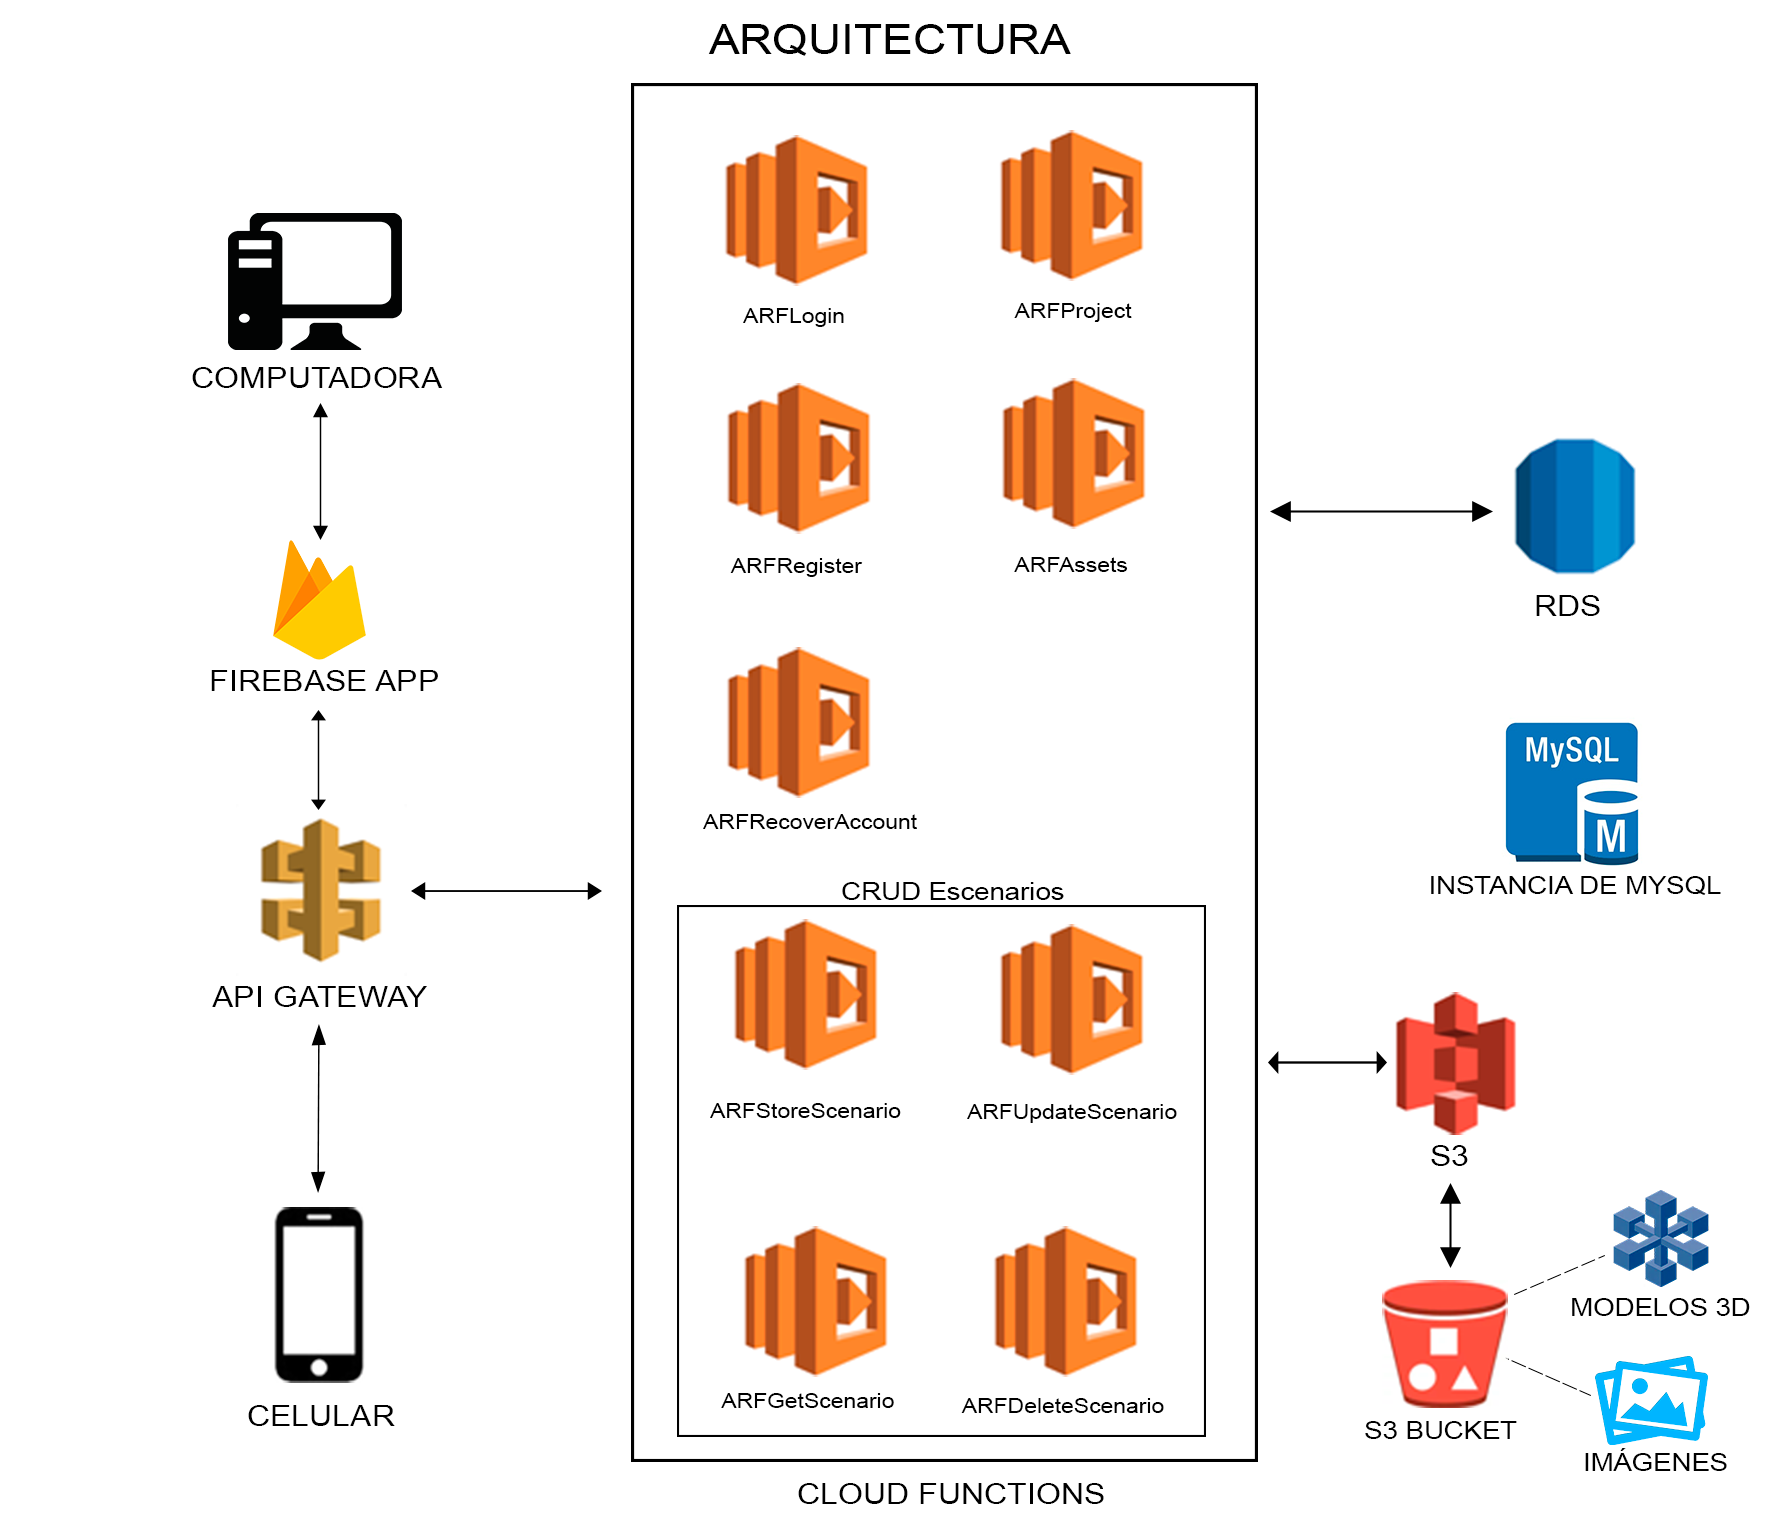
\includegraphics[width=15cm,height=15cm]{imagenes/desarrollo/arquitectura/ArchitecturaBackend.png}
	\caption{Arquitectura de Backend de ARF.}
	\label{fig:arqbackend}
\end{figure}
\par
Por otro lado se requerirá una base de datos que pueda almacenar los usuarios registrados y los escenarios que estos vayan creando. Para el tipo y cantidad de información que se requiere almacenar, una base de datos relacional cumple a ésta necesidad. En la figura  3.16 describe el diseño de la base de datos que se va a usar en ARF, misma que se encuentra en el clúster Amazon RDS mostrado en la figura 4.26.
\begin{figure}[H]
	\centering
	\includegraphics[width=10cm,height=7cm]{imagenes/desarrollo/arquitectura/ERD.png}
	\caption{Modelo Entidad-Relación usado para la base de datos de ARF.}
	\label{fig:arqbackend}
\end{figure}
		\section{Iteración I}
\subsection{Resumen}
\subsection{Diagramación}
\subsection{Desarrollo}


		\section{Iteración II}
\subsection{Resumen}
En esta iteración se modelo un mueble y se implementó para visualizarse en la aplicación.
\subsection{Desarrollo}
Ya entendido el funcionamiento de ARcore y como agregar nuevos modelos, en esta iteración se modelo el primer mueble, al igual que en la iteración pasada se obtuvieron dos tipos de archivos y se renderizaron para mostrarse en la aplicación.
\begin{figure}[H]
	\centering
	\includegraphics[width=8cm,height=14cm,angle=90]{imagenes/iteraciones/AR3.png}
	\caption{Mueble modelado en 3D}
	\label{fig:analogo}
\end{figure} 

		\section{Iteración III}
\subsection{Resumen}
En ésta iteración se realizó el frontend del login de ARF así como el backend para los módulos ``LOGIN", ``REGISTRAR CUENTA" y ``GUARDAR ESCENARIO" de acuerdo a la arquitectura descrita en la figura 4.25. \par

%\subsection{Diagramación}
\subsection{Desarrollo}
El desarrollo de los módulos de backend mencionados se realizó sobre Lambdas de AWS. Cada módulo tiene su propia función. El objetivo de hacerlo de esta forma es brindarle escalabilidad al sistema pues el desarrollo se logra de forma modular.\par
Cada uno de estos módulos es accesible a través del protocolo HTTP gracias a la API Gateway. La API Gateway es un módulo de Amazon Web Services que permite que los recursos de AWS sean accesibles desde el exterior, en éste caso, permite que la aplicación en Android pueda acceder a estas funciones con una simple petición. Asimismo las imágenes de los escenarios son almacenadas en AWS S3.\par

\subsubsection{Login}
Se encarga de la funcionalidad del login de la aplicación. En la figura 4.29 se puede observar el diagrama del proceso de login.\par
\begin{figure}[h!]
	\centering
	\includegraphics[width=15cm,height=9cm]{imagenes/desarrollo/diagramas/BPMN_LOGIN.png}
	\caption{Diagrama de proceso de Login.}
	\label{fig:loginsuccess}
\end{figure}

\subsubsection{Registro}
Ésta función se encarga de registrar un nuevo usuario en la base de datos para que posteriormente pueda iniciar sesión en la aplicación. El modelado de este proceso se puede apreciar en la figura 4.30. \par
\begin{figure}[h!]
	\centering
	\includegraphics[width=15cm,height=7cm]{imagenes/desarrollo/diagramas/BPMN_REGISTRAR_CUENTA.png}
	\caption{Proceso de registro de nuevo usuario.}
	\label{fig:regsuccess}
\end{figure}
\par

\subsubsection{Guardar escenario}
El objetivo de ésta función es poder almacenar los escenarios que vayan generando los usuarios para que después puedan ser visualizados desde la aplicación. En la figura 4.31 se puede apreciar el modelado del proceso de almacenamiento de escenario. \par
\begin{figure}[h!]
	\centering
	\includegraphics[width=13cm,height=7cm]{imagenes/desarrollo/diagramas/BPMN_STORESC.png}
	\caption{Proceso de guardado de escenario.}
	\label{fig:regsuccess}
\end{figure}
\clearpage
		\section{Iteración IV}
\subsection{Resumen}
En esta iteración se modelaron dos muebles más, tres botones para cambiar de modelo e implementamos un botón para tomar fotografía del escenario.
\subsection{Desarrollo}
Se modelaron dos muebles más, utilizando la misma herramienta, obteniendo los mismos archivos y realizando el proceso de las iteraciones I y II.

En la parte inferior de la aplicación se encuentran tres diseños de muebles, que funcionan como botones para seleccionar el objeto 3D que aparecerá en pantalla.

En la parte superior derecha de la aplicación tenemos ubicado un botón el cual toma una screenshot de la escena y la guarda en el dispositivo.

\begin{figure}[H]
	\centering
	\includegraphics[width=4cm,height=8cm]{imagenes/iteraciones/all.png}
	\caption{Aplicación: modelos en la parte inferior y botón de tomar foto parte superior}
	\label{fig:aplicacion}
\end{figure} 

Al presionar el botón "tomar fotografía" se guardará una imagen de la escena, en formato JPG y aparecerá un mensaje para abrir la ubicación de la imagen.  

\begin{figure}[H]
	\begin{minipage}{0.48\textwidth}
		\centering
		\includegraphics[width=5cm,height=10cm]{imagenes/iteraciones/save1.png}
		\caption{Pantalla de visualización de fotografías}
		\label{fig:save}
	\end{minipage}\hfill
	\begin{minipage}{0.48\textwidth}
		\centering
		\includegraphics[width=5cm,height=10cm]{imagenes/iteraciones/foto.jpg}
		\caption{Pantalla de registro nuevo usuario}
		\label{fig:foto}
	\end{minipage}\hfill
\end{figure}
Las interfaz que se muestra es temporal, se realizó de esta manera para probar la funcionalidad del aplicación al cumplir con algunos requerimientos funcionales, la interfaz final será como se muestra en los Mockups en la sección de \textbf{Anexos}
		%%%%%%%   BIBLIOGRAFÍA   %%%%%%%
%%		\chapter{Anexos}
\title
\section{Dieño de interfaces de usuario}
\begin{figure}[h!]
	\begin{minipage}{0.48\textwidth}
		\centering
		\includegraphics[width=4cm,height=8cm]{imagenes/Anexos/Mockup/1-Login.PNG}
		\caption{UI1 - Pantalla inicial de autenticación}
		\label{fig:analogo}
	\end{minipage}\hfill
	\begin{minipage}{0.48\textwidth}
		\centering
		\includegraphics[width=4cm,height=8cm]{imagenes/Anexos/Mockup/2-principalSinLogin.png}
		\caption{UI2 - Pantalla principal sin autenticación}
		\label{fig:analogo}
	\end{minipage}\hfill
\end{figure}

\begin{figure}[h!]
	\begin{minipage}{0.48\textwidth}
		\centering
		\includegraphics[width=4cm,height=8cm]{imagenes/Anexos/Mockup/3-MenuMuebles.PNG}
		\caption{UI3 - Menú desplegable de muebles (catalogo)}
		\label{fig:analogo}
	\end{minipage}\hfill
	\begin{minipage}{0.48\textwidth}
		\centering
		\includegraphics[width=4cm,height=8cm]{imagenes/Anexos/Mockup/4-principalLogin.png}
		\caption{UI4 - Pantalla principal tras autenticación}
		\label{fig:analogo}
	\end{minipage}\hfill
\end{figure}

\begin{figure}[h!]
	\begin{minipage}{0.48\textwidth}
		\centering
		\includegraphics[width=4cm,height=8cm]{imagenes/Anexos/Mockup/5-GuardarEscenario.PNG}
		\caption{UI5 - Pantalla de almacenamiento de escenario}
		\label{fig:analogo}
	\end{minipage}\hfill
	\begin{minipage}{0.48\textwidth}
		\centering
		\includegraphics[width=4cm,height=8cm]{imagenes/Anexos/Mockup/6-MisEscenarios.PNG}
		\caption{UI6 - Pantalla de visualización de escenarios }
		\label{fig:analogo}
	\end{minipage}\hfill
\end{figure}

\begin{figure}[h!]
	\begin{minipage}{0.48\textwidth}
		\centering
		\includegraphics[width=4cm,height=8cm]{imagenes/Anexos/Mockup/7-Foto.PNG}
		\caption{UI7 - Pantalla de visualización de fotografías}
		\label{fig:analogo}
	\end{minipage}\hfill
	\begin{minipage}{0.48\textwidth}
		\centering
		\includegraphics[width=4cm,height=8cm]{imagenes/Anexos/Mockup/8-Registro.PNG}
		\caption{UI8 - Pantalla de registro nuevo usuario}
		\label{fig:analogo}
	\end{minipage}\hfill
\end{figure}

\begin{figure}[h!]
	\begin{minipage}{0.48\textwidth}
		\centering
		\includegraphics[width=4cm,height=8cm]{imagenes/Anexos/Mockup/9-RecuperarP.PNG}
		\caption{UI9 - Pantalla de recuperación de contraseña 1}
		\label{fig:analogo}
	\end{minipage}\hfill
	\begin{minipage}{0.48\textwidth}
		\centering
		\includegraphics[width=4cm,height=8cm]{imagenes/Anexos/Mockup/10-RecuperarP2.PNG}
		\caption{UI10 - Pantalla de recuperación de contraseña 2}
		\label{fig:analogo}
	\end{minipage}\hfill
\end{figure}

\begin{figure}[h!]
	\begin{minipage}{0.48\textwidth}
		\centering
		\includegraphics[width=4cm,height=8cm]{imagenes/Anexos/Mockup/11-ActualizarP.PNG}
		\caption{UI11 - Pantalla de actualización de contraseña}
		\label{fig:analogo}
	\end{minipage}\hfill
	\begin{minipage}{0.48\textwidth}
		\centering
		\includegraphics[width=4cm,height=8cm]{imagenes/Anexos/Mockup/12-VerEscenario.PNG}
		\caption{UI12 - Pantalla de visualización de imágenes de escenario }
		\label{fig:analogo} 
	\end{minipage}\hfill
\end{figure}   
	%%%%%%%   BIBLIOGRAFÍA   %%%%%%%
	\begin{thebibliography}{X}
	
	\bibitem{B15} \textsc{Hsu, Pei-Hsien}, \textsc{Huang, Sheng-Yang} y \textsc{Lin, Bao-Shuh} ``Smart-Device-Based Augmented Reality (SDAR) Models to Support Interior Design: Rethinking ``Screen” in Augmented Reality", National Chiao Tung University, Taiwan
	
	\bibitem{B01} \textsc{Montes de Oca, Irina} y \textsc{Risco, Lucía},
	``Apuntes de diseño de interiores",
	\textit{Principios básicos de escalas. espacios, colores y más}, primera edicion,
	ECOE EDICIONES
	
	\bibitem{B02} ``FAQ for designers", \textit{Whats is Interior Design}, Interior Design Legislative Coalition of Pennsylvania (IDLCPA), 2011. Recuperado de: https://www.idlcpa.org/forms/resources/FAQforDesigners.pdf
	
	%\bibitem{B26} Kathryn, T.,(2000), feng shui habitación por habitación (12ª ed.). ES, Urano.	
	
	%\bibitem{B24} Harris, C., (2006), dictionary of architecture and construction (4ª ed.). New York, EU, McGraw-Hill.
	
		
	\bibitem{B13} \textsc{Viola, Romina} (11 de mayo de 2016), ``Cómo Elegir la Paleta de Colores", \textit{Parte I: Entender el Color}. Spanish Community Champion | Piktochart. [Online] Recuperado de: https://piktochart.com/es/blog/como-elegir-la-paleta-de-colores-parte-entender-el-color/
	
	
	
	\bibitem{B04} \textsc{Siltanen, Sanni} ``Diminished reality for augmented reality interior design", Springer-Verlag Berlin Heidelberg 2015. Publicado el: 30 de Noviembre de 2015. DOI: 10.1007/s00371-015-1174-z
	DOI 10.1007/978-3-319-54502-8
	
	\bibitem{B05} \textsc{Donggang Yu1, Jesse Sheng Jina},
	``A Useful Visualization Technique: A Literature Review for Augmented Reality and its Application, limitation and future direction", primera edicion,
	School of Design, Communication and Information Technology, The University of Newcastle, Callaghan, NSW 2308, Australia
	
	
	
	\bibitem{B27} \textsc{Furht, Borko} ``Handbook of Augmented Reality",Department of Computer and Electrical Engineering and Computer Science,Florida Atlantic University (),Glades Road 777 33431 Boca Raton, Florida USA,DOI 10.1007/978-1-4614-0064-6
	
	\bibitem{B22} \textsc{Peddie, Jon} ``Augmented Reality Where we will all live", Springer International Publishing AG 2017. Publicado el: 19 de Abril del 2017. DOI 10.1007/978-3-319-54502-8 
	
	\bibitem{B09} \textsc{Monteiro, Paula} and \textsc{Nagele, Aleksandra}, ``Wikitude" \textsc{Company Overview}, Recuperado de: https://s3-eu-west-1.amazonaws.com/wikitude-web-hosting/static-website/2017/07/01728364/Media+page+presentation+-+Wikitude.pdf
	
	
	
	\bibitem{B16} ``Wikitude Products", 29 de agosto de 2018. Recuperado de: https://www.wikitude.com/products/wikitude-sdk/
	
	
	\bibitem{B20} ``ARKit Developer", 2 de Septiembre de 2018. Recuperado de:
	https://developer.apple.com/arkit/
	
	\bibitem{B21} ``ARKit Documentation", 3 de Septiembre de 2018. Recuperado de:
	https://developer.apple.com/documentation/arkit/
	
	
	\bibitem{B12} \textsc{Grahn, Ivar}, ``The Vuforia SDK and Unity3D Game Engine", \textit{Evaluating performanceo on Android Devices}. Linköping University | Department of Computer and Information, Science Bachelor thesis, 16 ECTS, Computer Science 2017, LIU-IDA/LITH-EX-G–17/059–SE
	
	
	\bibitem{B14} ``ARCore Overview", 2 de agosto de 2018. Recuperado de: https://developers.google.com/ar/discover/
	\\
	
	
	%
	
	\bibitem{B03} \textsc{Takahashi, Yoshiyuki} y \textsc{Mizumura, Hiroko},
	``Augmented Reality Based Environment Design Support System for Home Renovation", Toyo  University, Department of Human Environment Design, Faculty of Human Life Design, Oka 48-1, Asaka-shi, Saitama, 351-8510 Japan 
	
	
	
	\bibitem{B06} \textsc{Buerli, Mike} and \textsc{Misslinger, Stefan}, ``Introducing ARKit", \textit{Augmented Reality for iOS. Session 602} Recuperado de: https://devstreaming-cdn.apple.com/videos/wwdc/2017/602pxa6f2vw71ze/602/602
	\_introducing\_arkit\_augmented\_reality\_for\_ios.pdf?dl=1
	
	\bibitem{B07} \textsc{Strandmark, Petter}, ``Augmented reality with the ARToolKit", Recuperado de: http://www.maths.lth.se/matematiklth/personal/petter/rapporter/artoolkit4.pdf
	
	\bibitem{B08} \textsc{Fuster Andújar, Francisco de Asís}, ``Aplicación Android de realidad aumentada para mostrar imágenes históricas de lugares turísticos de interés", Tesis. Escola Tècnica Superior d’Enginyeria Informàtica Universitat Politècnica de València, Valencia, España, 2014.
	
	
	\bibitem{B10} \textsc{Asrul Sani, Nisfu}, ``Google ARCore", Lab Langit 9 - PENS 20-22 de noviembre de 2017. Recuperado de: http://dhoto.lecturer.pens.ac.id/training/arcore/SONI-ARCORE.pdf
	
	\bibitem{B11} \textsc{Kaleda, Yuliya}, ``Add Reality to App with ARCore". Recuperado de: https://downloads.ctfassets.net/2grufn031spf/7AyZDCxxIs0AoOgwOsy0m4/26f89f9d2
	f346dd3c6a55f5d3e2de96e/Yuliya\_Kaleda\_Add\_Reality\_To\_App\_with\_ARCore.pdf
	

	
	
	
	\bibitem{B18} ``OpenGL Documentation". Recuperado el 30 de agosto de 2018 de: https://www.opengl.org/documentation/
	
	\bibitem{B19} ``OpenGL Glut". Recuperado el 30 de agosto de 2018 de: https://www.opengl.org/resources/libraries/glut/spec3/spec3.html
	
    
	
	\bibitem{B23} ``Vuforia Supported-devices". Recuperado el 4 de Septiembre de 2018 de: https://library.vuforia.com/articles/Solution/vuforia-fusion-supported-devices.html
	
	\bibitem{B25} Medina, V. E., (2003). Forma y composición en la arquitectura descontructivista (Tesis doctoral). Escuela Técnica Superior de Arquitectura de Madrid, Madrid, Esp.
	
	\bibitem{B28} ``The new power tool for home improvement". Recuperado el 22 de Octubre de 2018 de: https://canvas.io/
	\bibitem{B29} ``Fingo. Furniture. Try before you buy!". Recuperado el 22 de Octubre de 2018 de: https://itunes.apple.com/us/app/fingo.vybor-mebeli-katalog/id845105741
	\bibitem{B30} ``Electronics -AGILE - Agile Software Technologies". \textit{Mobile -D}. Recuperado el 23 de Octubre de 2018 de: https://itunes.apple.com/us/app/fingo.vybor-mebeli-katalog/id845105741
	
	
\end{thebibliography}

	
	
\end{document}


%%%%%%%%%%%%%%%%%%%%%%%%%%%%%%%%%%%%%%%
%%%%%%%    FIN DEL DOCUMENTO    %%%%%%%
%%%%%%%%%%%%%%%%%%%%%%%%%%%%%%%%%%%%%%%
